\section{Objects}
\label{sec:objects}
This analysis follows the same object defintion as in \cite{CMS:2019chr} for each year. Detailed descricption on objection definitions and scale factors can be found in the corresponding analysis note ~\cite{CMS-PAS-HIG-19-001}. Since this analysis is based on Ultra Legacy (UL) full Run 2 data, most of the objects related ingredients will be reevaluated with respect to ~\cite{CMS-PAS-HIG-19-001}.     

The reconstruction of the SM Higgs boson in the decay chain $\HZZfl$ requires very efficient lepton reconstruction and identification in order to be sensitive
to a low mass Higgs, for which at least one of the leptons has a $p_T$ within the range 5 - 15~GeV. In this kinematic region the need is for an optimal
efficiency, while retaining the rate of misidentified leptons low enough. On the same time, to allow a precise measurement of the Higgs boson mass and together
properties, which depend on the lepton kinematics, the analysis needs a precise momentum measurement. For both reasons, the analysis will make use of high
statistics sources of prompt leptons to measure efficiency, mis-identification rate, and energy scale/resolution. Muon Efficiency measuremens using UL dataset are discribed as follows:

%In this chapter we describe the selection of leptons and jets and the calibrations done on data control samples relevant for this analysis.
%
\subsection{Electrons}

%\subsubsection{Electron Reconstruction}
\subsubsection{Electron Reconstruction and Identification}
\label{sec:eleReco}
Referred to \cite{CMS-PAS-HIG-19-001}.

%More details on electron reconstruction can be found in Ref.~\cite{ElectronLegacy}. 
%
%Electron candidates are preselected using loose cuts on track-cluster matching observables, so as to preserve the highest possible efficiency while rejecting part of the QCD background. To be considered for the analysis, electrons are required to have a
%transverse momentum $p^e_T >$ 7 GeV, a reconstructed $|\eta^e| <$ 2.5, and to satisfy a loose primary vertex 
%constraint defined as $d_{xy} < 0.5$ cm and $d_z < 1$ cm.
%Such electrons are called {\bf loose electrons}.
%
%The data-MC discrepancy is corrected using scale factors as is done for the electron selection with data efficiencies measured using the same tag-and-probe technique outlined later (see Section~\ref{sec:eleEffMeas}). 
%These studies for reconstructions are carried out by the EGM POG and the results are only summarised here.
%
%The electron reconstruction scale factors are shown Fig.~\ref{fig:ele_rec_scale_factors} and are applied as a function of the super cluster $\eta$ and electron $\pt$.
%
%\begin{figure}[!htb]
%\vspace*{0.3cm}
%\begin{center}
%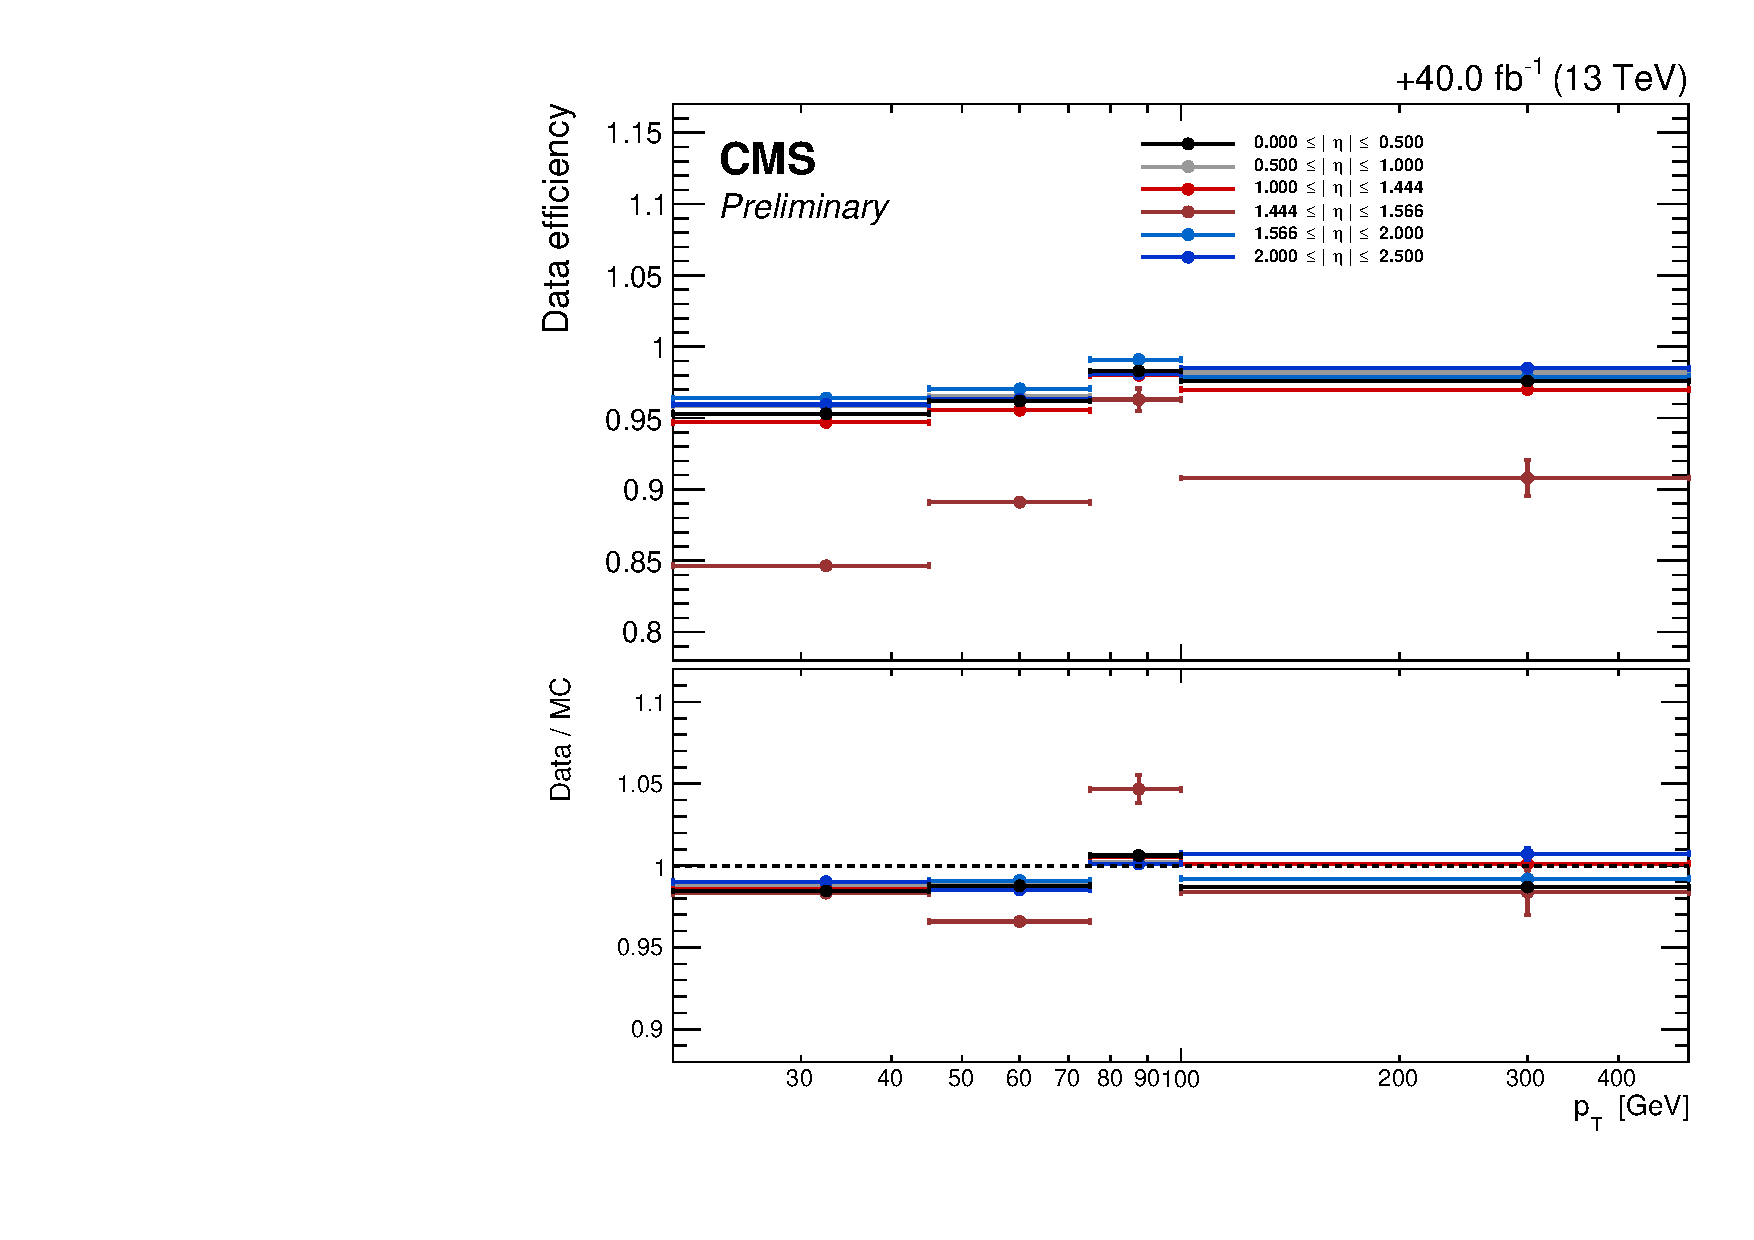
\includegraphics[width=0.4\textwidth]{Figures/Electrons/ErecoPt}
%\includegraphics[page=2, width=0.4\textwidth]{Figures/Electrons/ErecoEta}\\
%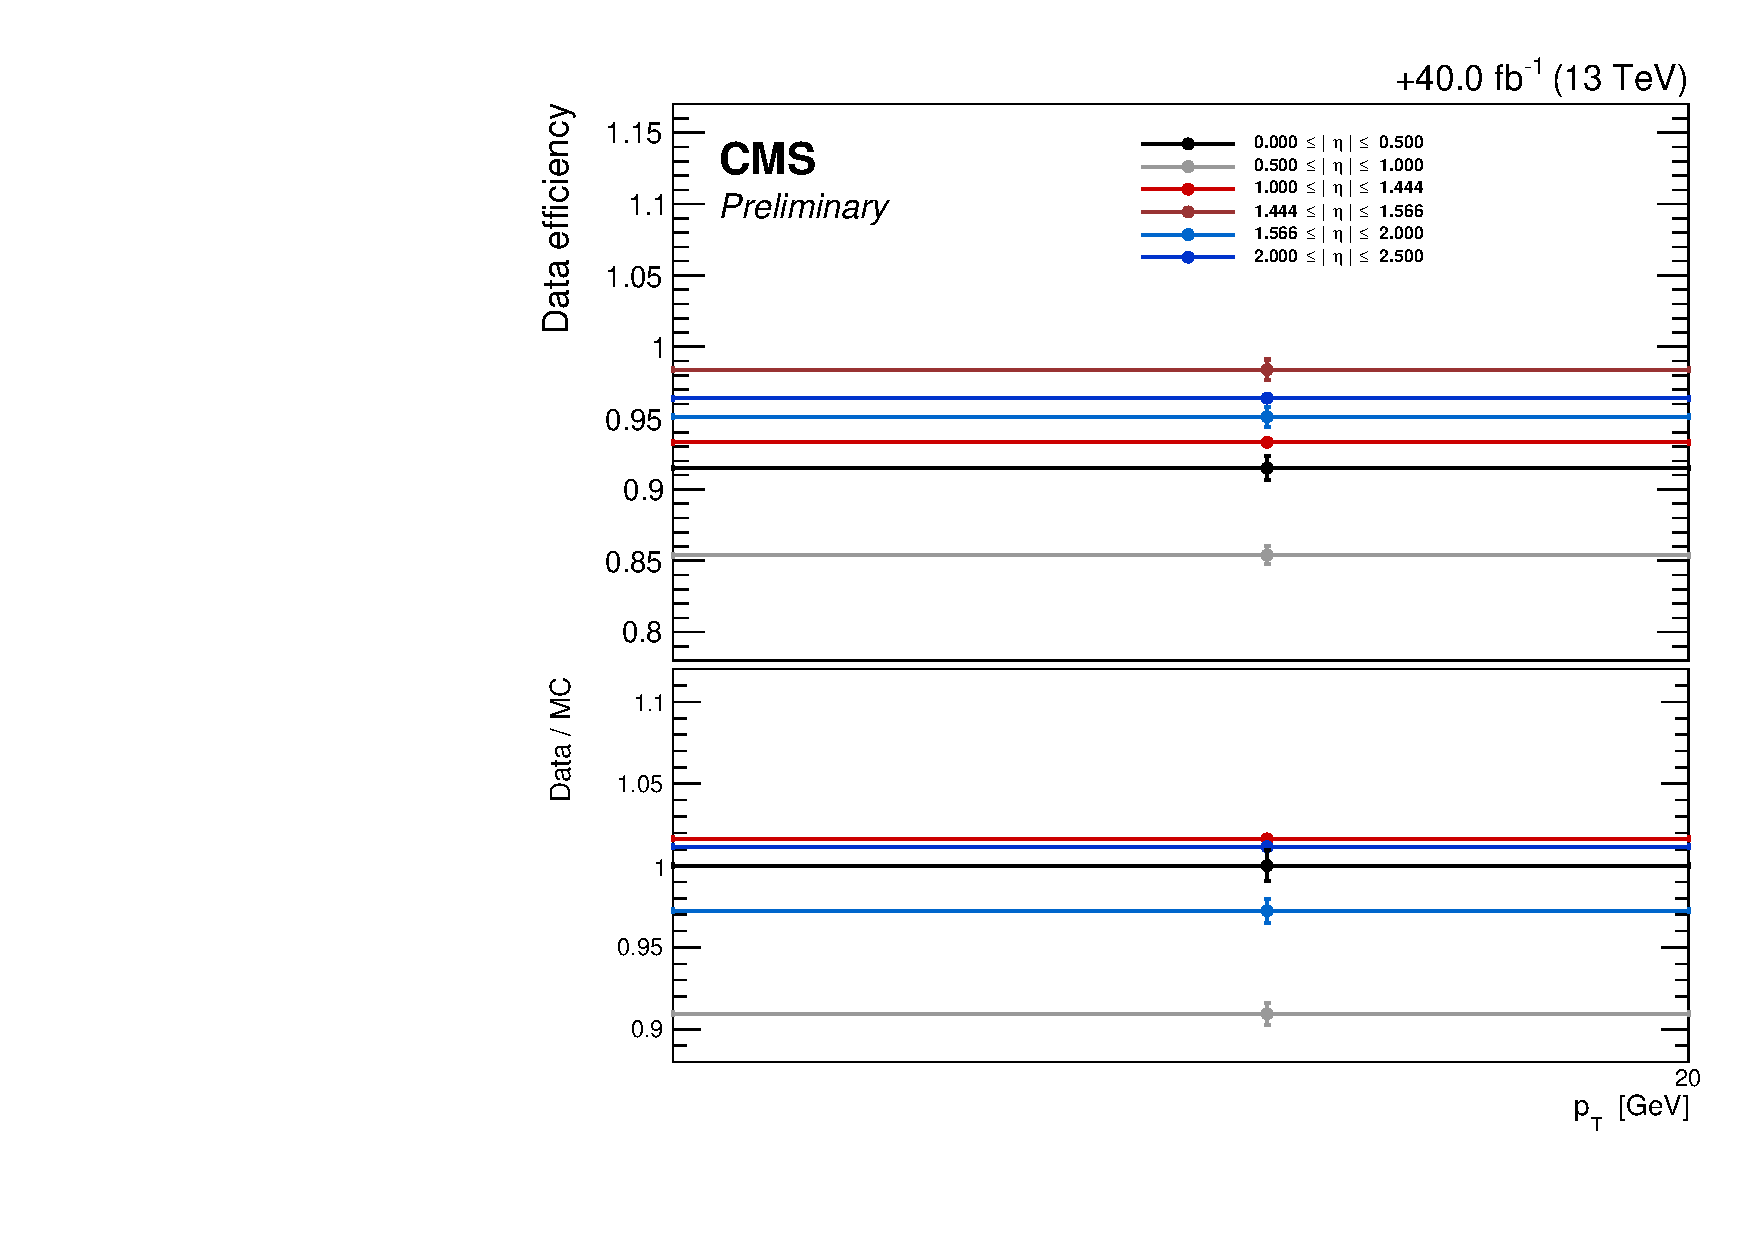
\includegraphics[width=0.4\textwidth]{Figures/Electrons/ErecoPt_lowPt}
%%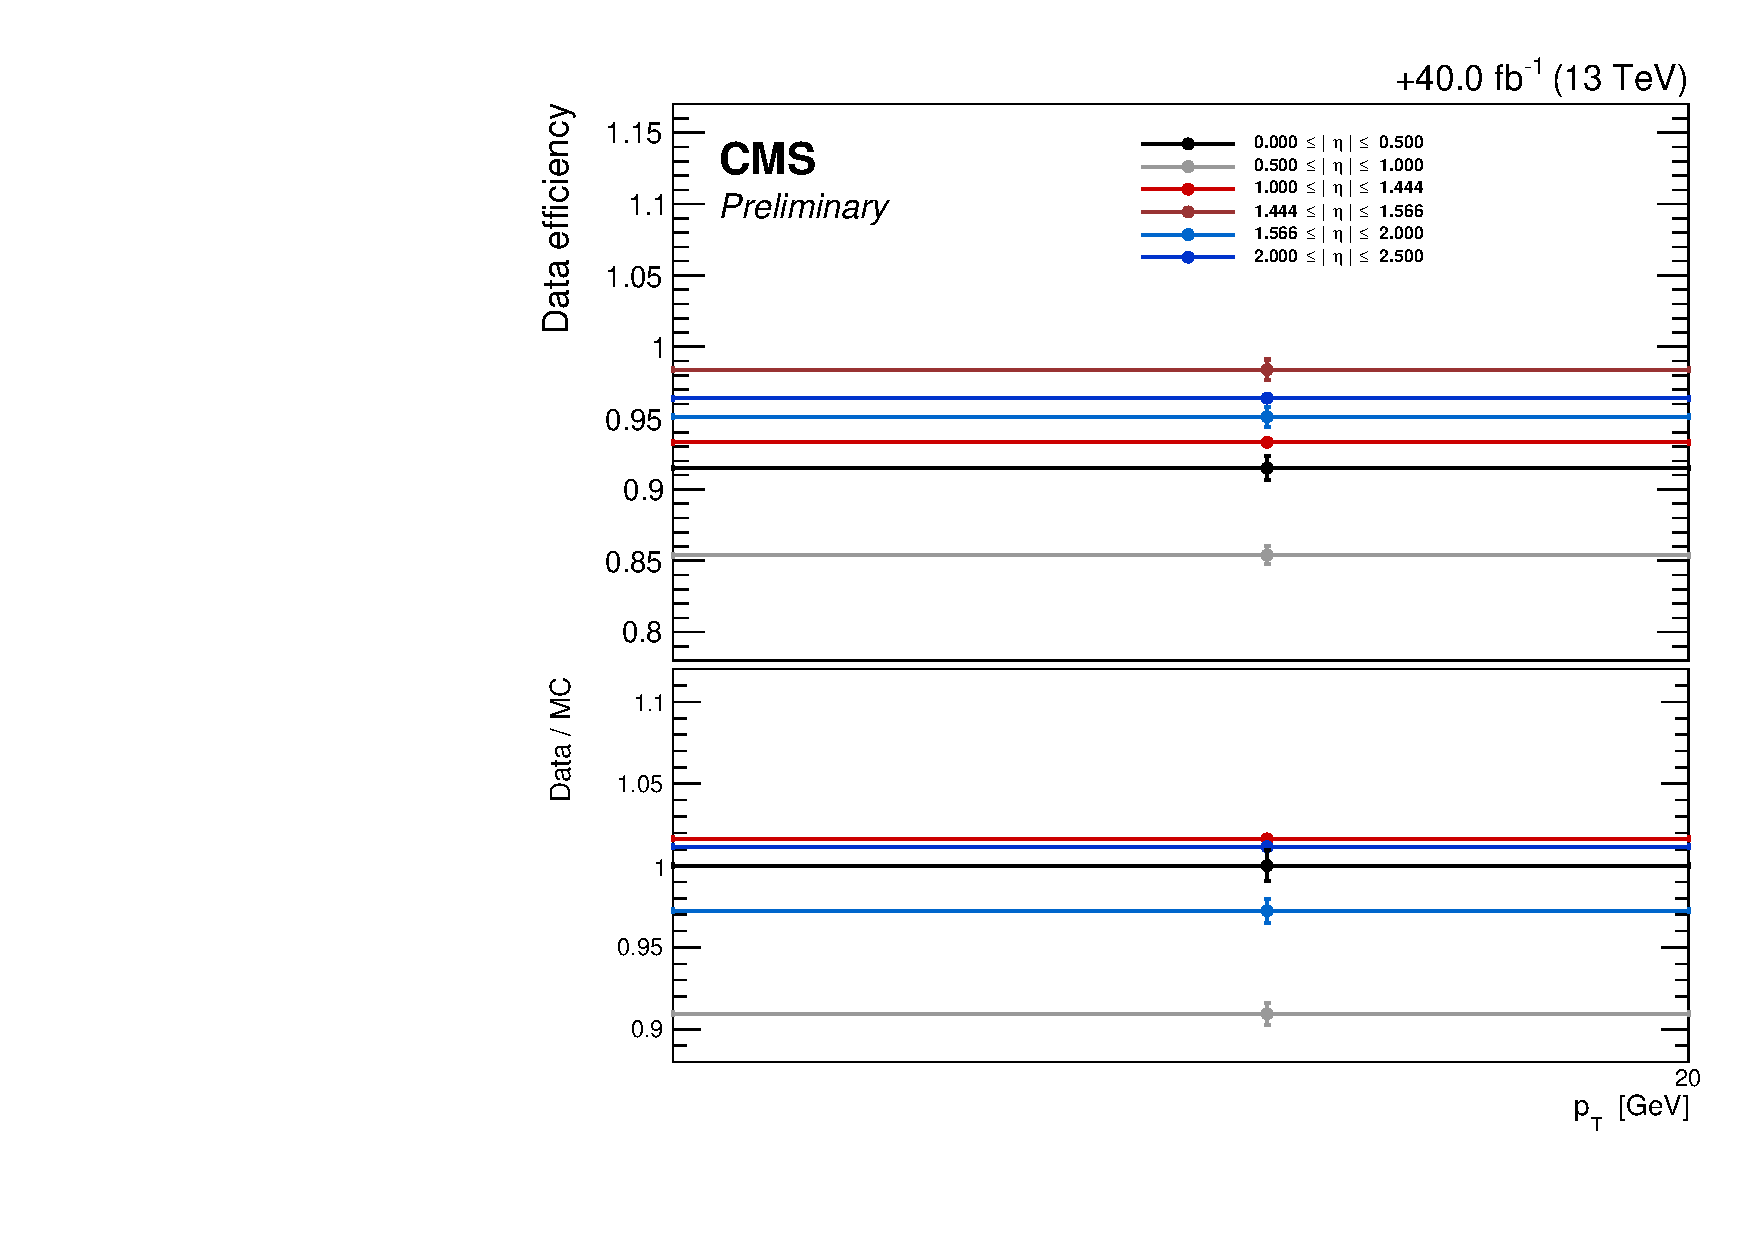
\includegraphics[width=0.4\textwidth]{Figures/Electrons/ErecoEta_lowPt}
%\end{center}
%\caption{Electron reconstruction efficiencies efficiency in data versus $p_T$ (left) and $\eta$ (right) for electrons with $\pt > 20 \GeV$ (top) and $\pt < 20 \GeV$ (bottom) with corresponding data/MC scale factors as provided by the EGM POG. Errors are statistical only. }
%\label{fig:ele_rec_scale_factors}
%\end{figure}
%


%
%\subsubsection{Electron Identification and Isolation}
%\label{sec:ele_MVA}
%One of the main improvements brought in the analysis is the usage of a new multivariate discriminant for electron selection in all data taking periods.

Reconstructed electrons are now identified and isolated by means of an e\textbf{X}treme \textbf{G}radient \textbf{Boost}ing (XGBoost) optimized distributed
gradient boosting library designed to be highly efficient, flexible and portable. It implements machine learning algorithms under the Gradient Boosting framework
and exploits observables from the electromagnetic cluster, the matching between the cluster and the electron track, observables based exclusively on tracking
measurements as well as particle flow isolation sums. The full list of used features can be found in the Table~\ref{tab:ele_ID_input_variables}.

\begin{table}[H]
\scriptsize
   \centering
   \begin{tabular}{c|l}
\hline
\hline
Observable type & Observable name \\
\hline
\multirow{6}{*}{Cluster shape}
	& RMS of the energy-crystal number spectrum along $\eta$ and $\varphi$; $\sigma_{i\eta i\eta}$, $\sigma_{i\varphi i\varphi}$ \\
	& Super cluster width along $\eta$ and $\phi$ \\
	& Ratio of the hadronic energy behind the electron supercluster to the supercluster energy, $H/E$ \\
	& Circularity $(E_{5\times5} - E_{5\times1})/E_{5\times5}$ \\
	& Sum of the seed and adjacent crystal over the super cluster energy $R_{9}$ \\
	& For endcap traing bins: energy fraction in pre-shower $E_\text{PS}/E_\text{raw}$ \\
\hline
\multirow{2}{*}{Track-cluster matching}
	& Energy-momentum agreement $E_{tot}/p_{in}$, $E_{ele}/p_{out}$, $1/E_{tot} - 1/p_{in}$ \\
	& Position matching $\Delta\eta_{in}$, $\Delta\varphi_{in}$, $\Delta\eta_{seed}$ \\
\hline
\multirow{5}{*}{tracking}
   & Fractional momentum loss $f_{brem} = 1 - p_{out}/p_{in}$ \\
   & Number of hits of the KF and GSF track $N_{KF}$, $N_{GSF}$ \\ %$(\mathord{\cdot})$ \\
   & Reduced $\chi^2$ of the KF and GSF track $\chi^{2}_{KF}$, $\chi^{2}_{\textrm{GSF}}$ \\
   & Number of expected but missing inner hits \\ %$(\mathord{\cdot})$ \\
   & Probability transform of conversion vertex fit $\chi^2$ \\ % $(\mathord{\cdot})$ \\
\hline
\multirow{3}{*}{isolation}
   & Particle Flow photon isolation sum \\ %$(\mathord{\cdot})$ \\
   & Particle Flow charged hadrons isolation sum \\ %$(\mathord{\cdot})$ \\
   & Particle Flow neutral hadrons isolation sum \\ %$(\mathord{\cdot})$ \\
\hline
\multirow{1}{*}{For PU-resilience}
   & Mean energy density in the event: $\rho$ \\ %$(\mathord{\cdot})$ \\
\hline
\hline
     \end{tabular}
\small
    \caption{Overview of input features to the identification classifier.} %Variables not used in the Run 2 MVA are marked with  $(\mathord{\cdot})$.}
    \label{tab:ele_ID_input_variables}
\end{table}


The model is trained on 2016, 2017, and 2018 Drell-Yan with jets MC sample for both signal and background. The separate training for three periods guarantees
optimal performance during the whole Run 2 data taking period. The simulated samples used to train the model are listed bellow.

\begin{itemize}
\item \textbf{2016} \begin{verbatim}/DYJetsToLL_M-50_TuneCUETP8M1_13TeV-amcatnloFXFX-pythia8/RunIISummer16MiniAODv2-PUMoriond17_80X_mcRun2_asymptotic_2016_TrancheIV_v6_ext2-v1/MINIAODSIM\end{verbatim}
\item \textbf{2017} \begin{verbatim}/DYJetsToLL_M-50_TuneCP5_13TeV-madgraphMLM-pythia8/RunIIFall17MiniAOD-RECOSIMstep_94X_mc2017_realistic_v10-v1/MINIAODSIM\end{verbatim}
\item \textbf{2018} \begin{verbatim}/DYJetsToLL_M-50_TuneCP5_13TeV-madgraphMLM-pythia8/RunIIAutumn18MiniAOD-102X_upgrade2018_realistic_v15-v1/MINIAODSIM\end{verbatim}
\end{itemize}

Several studies have been conducted on 2016 Drell-Yan with jets MC sample. The XGBoost framework was first used in 2017 and the model was trained on 2017
Drell-Yan with jets MC sample. This model is known as 2017 ID+ISO V2. The same framework was then used to train the model on 2016 MC (2016 ID+ISO) and finally
on 2018 MC (2018 ID+ISO). In Fig.~\ref{fig:ele_ID_ISO_ROC_2016} one can see the ROC curves obtained using 2016 Drell-Yan with jets MC sample. As expected, the
model trained on 2016 MC using electron identification and isolation features outperforms the model trained on 2016 MC using only identification features and
the model obtained after applying 2017 ID+ISO V2 training on 2016 Drell-Yan with jets MC sample.

In Fig.~\ref{fig:ele_ID_ISO_ROC_2016_} one can see the ROC curve for the model trained on 2016 MC using electron identification and isolation features and ROC
curve when applying sequential approach meaning applying isolation cut after cutting on the distribution obtained by training using only identification features.
As expected, the model obtained using electron identification and isolation features outperforms the sequential approach model.

\begin{figure}[!htb]
   \vspace*{0.3cm}
   \begin{center}
      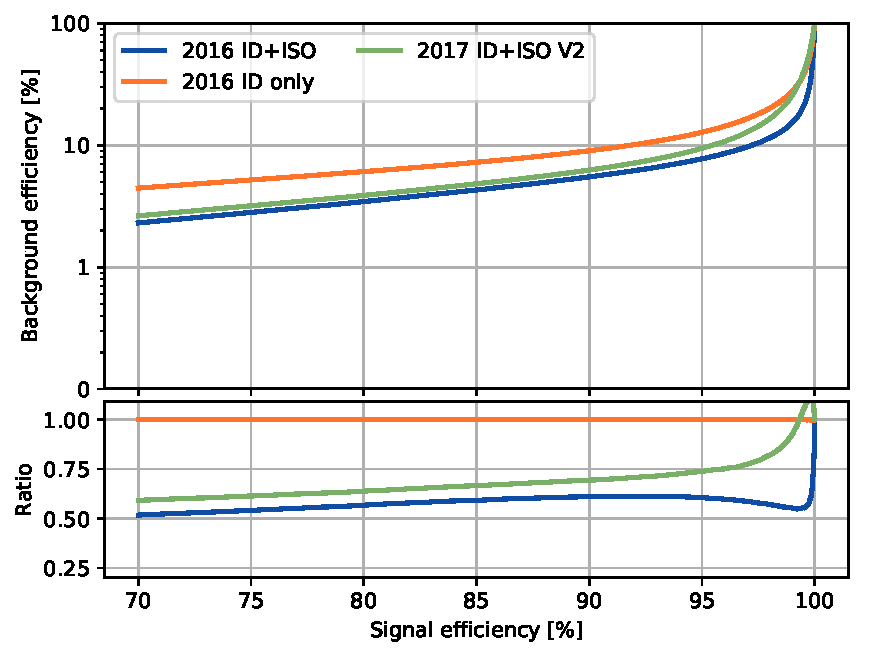
\includegraphics[width=0.45\textwidth]{Figures/Electrons/2016_EB1_5.pdf}
      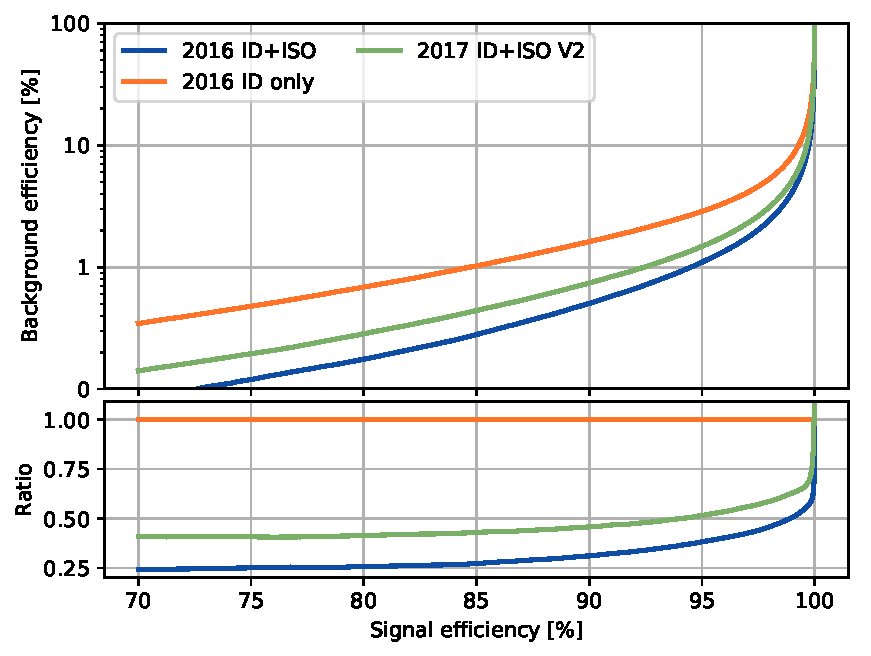
\includegraphics[width=0.45\textwidth]{Figures/Electrons/2016_EB1_10.pdf} \\
      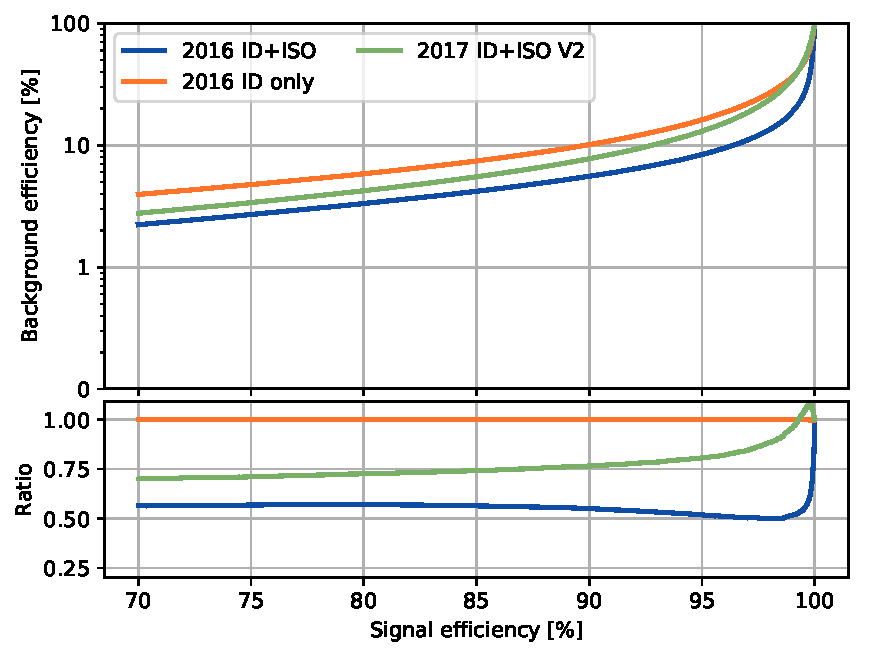
\includegraphics[width=0.45\textwidth]{Figures/Electrons/2016_EB2_5.pdf}
      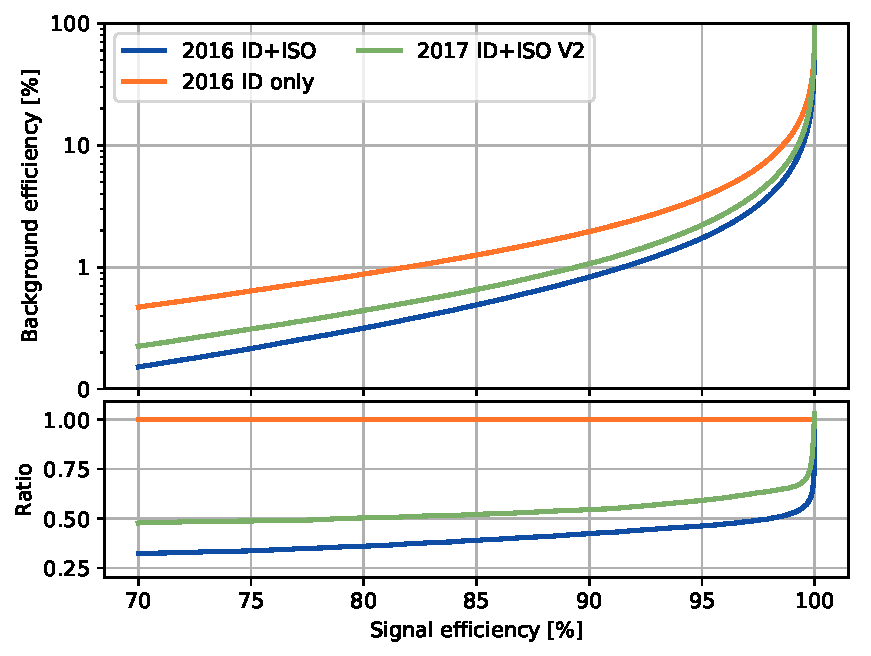
\includegraphics[width=0.45\textwidth]{Figures/Electrons/2016_EB2_10.pdf} \\
      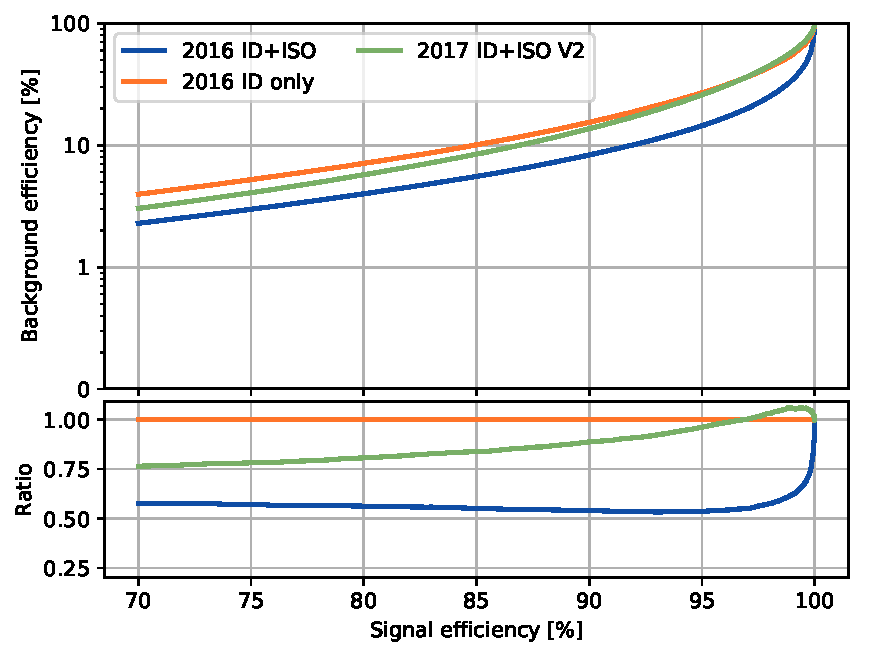
\includegraphics[width=0.45\textwidth]{Figures/Electrons/2016_EE_5.pdf}
      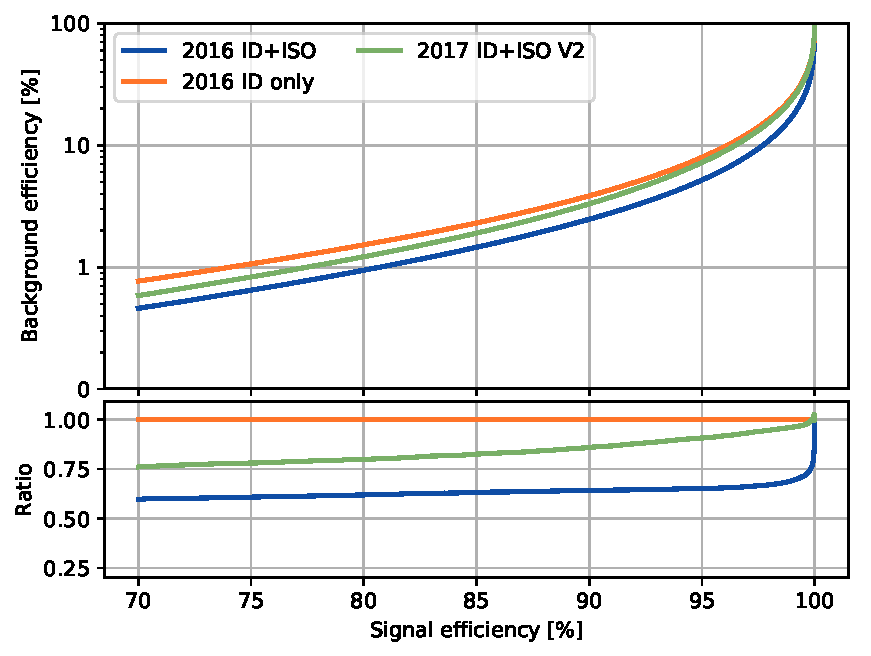
\includegraphics[width=0.45\textwidth]{Figures/Electrons/2016_EE_10.pdf} \\
   \caption{The receiver operating characteristic curves, representing the background efficiency vs signal efficiency, of the MVA trained on 2016 Drell-Yan with
   jets MC sample. Performance are shown for electrons with $5 < p_T < 10 $ GeV (left), $p_T > 10$ GeV (right), and $|\eta| < 0.8$ (top),
   $0.8 < |\eta| < 1.479$ (middle), and $|\eta| > 1.479$ (bottom).
   \label{fig:ele_ID_ISO_ROC_2016}}
   \end{center}
\end{figure}


\begin{figure}[!htb]
   \vspace*{0.3cm}
   \begin{center}
      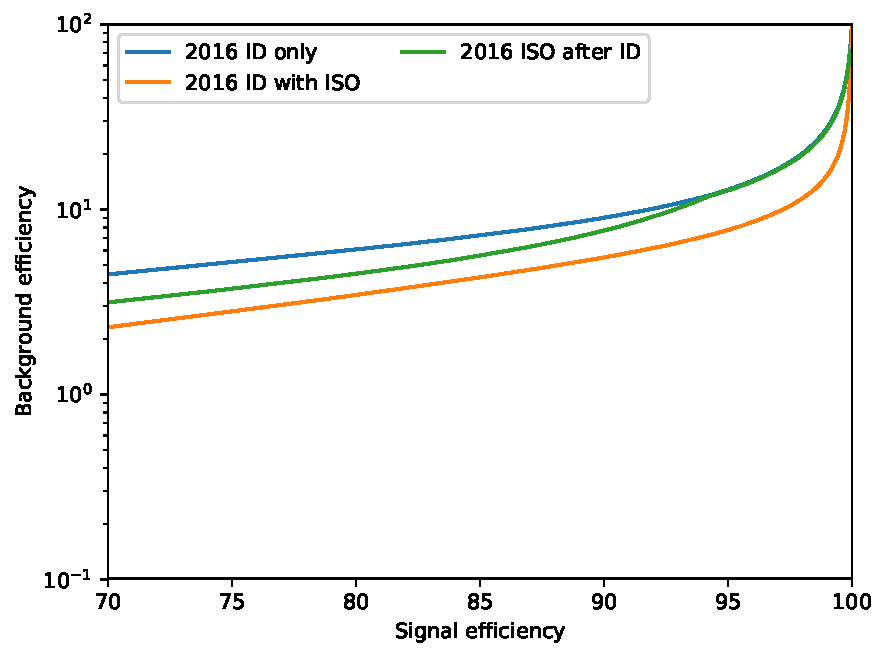
\includegraphics[width=0.45\textwidth]{Figures/Electrons/2016_EB1_5_.pdf}
      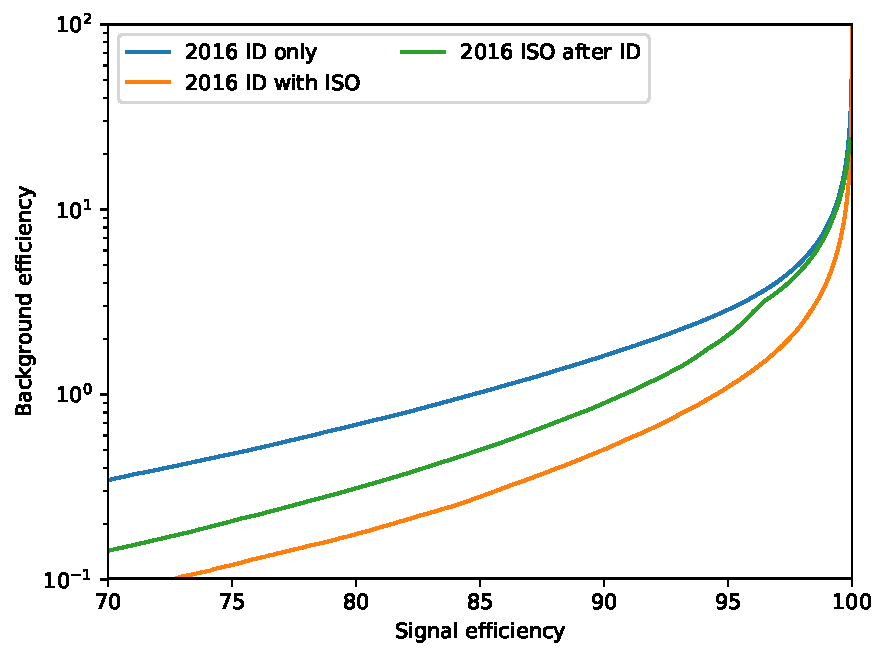
\includegraphics[width=0.45\textwidth]{Figures/Electrons/2016_EB1_10_.pdf} \\
      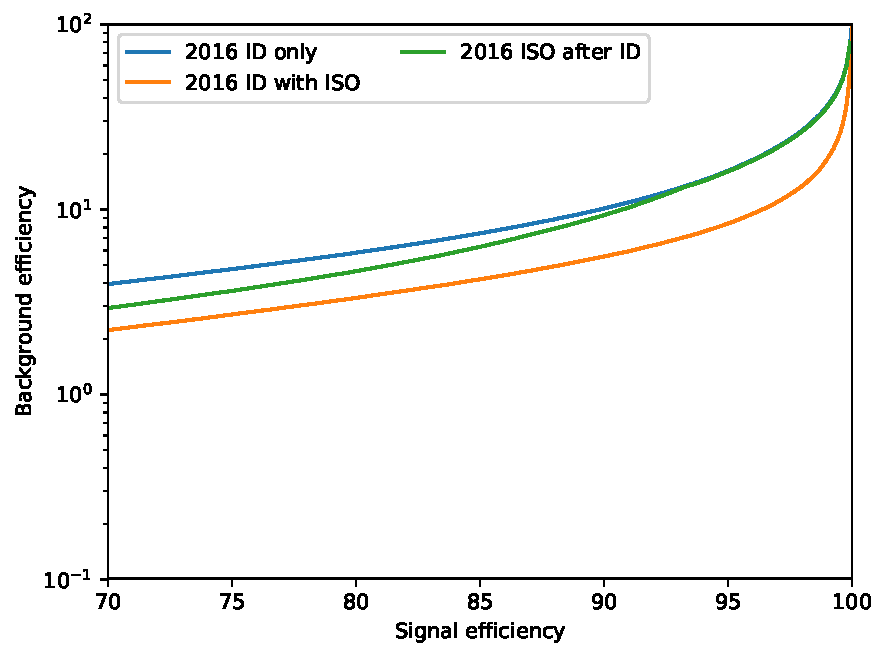
\includegraphics[width=0.45\textwidth]{Figures/Electrons/2016_EB2_5_.pdf}
      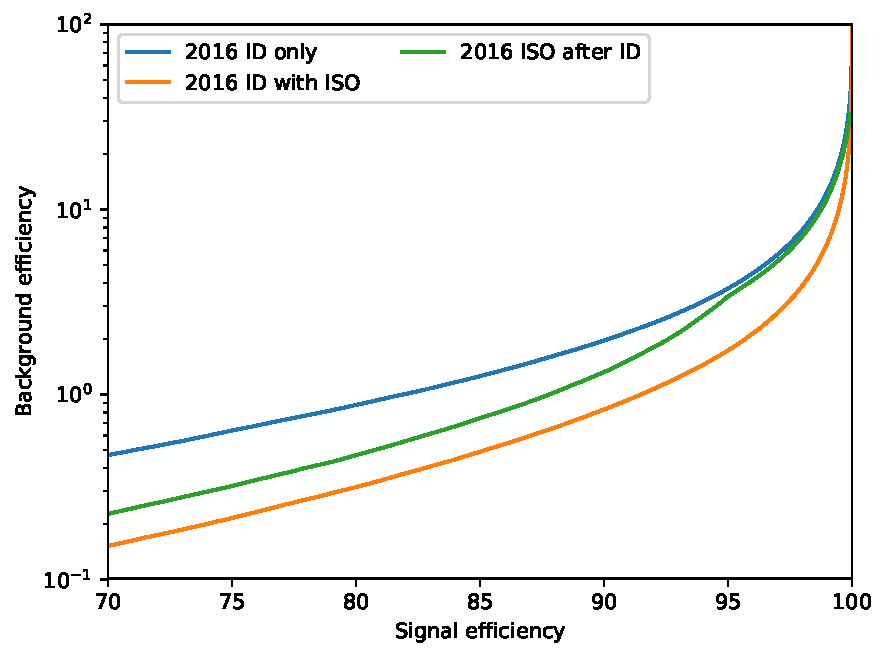
\includegraphics[width=0.45\textwidth]{Figures/Electrons/2016_EB2_10_.pdf} \\
      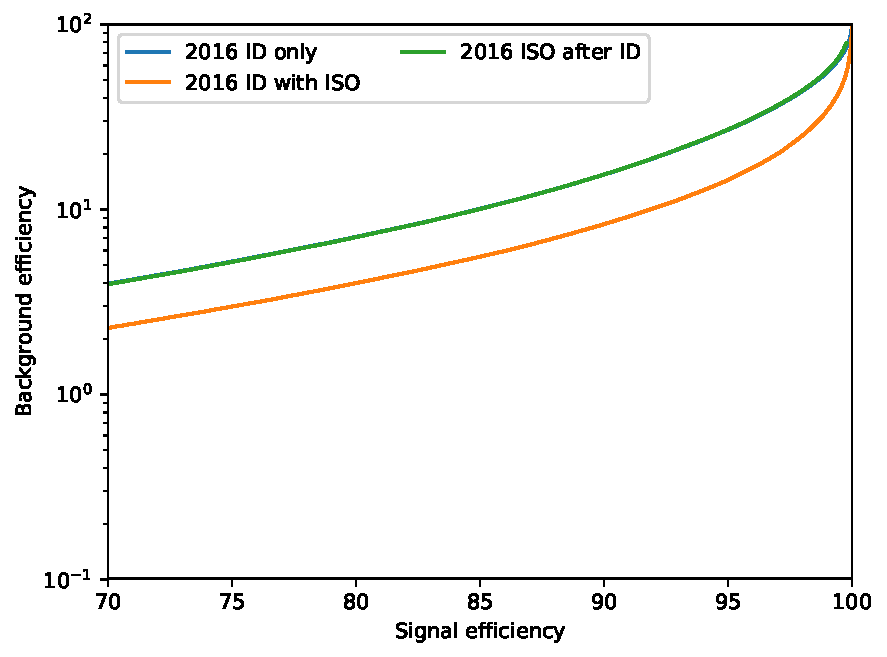
\includegraphics[width=0.45\textwidth]{Figures/Electrons/2016_EE_5_.pdf}
      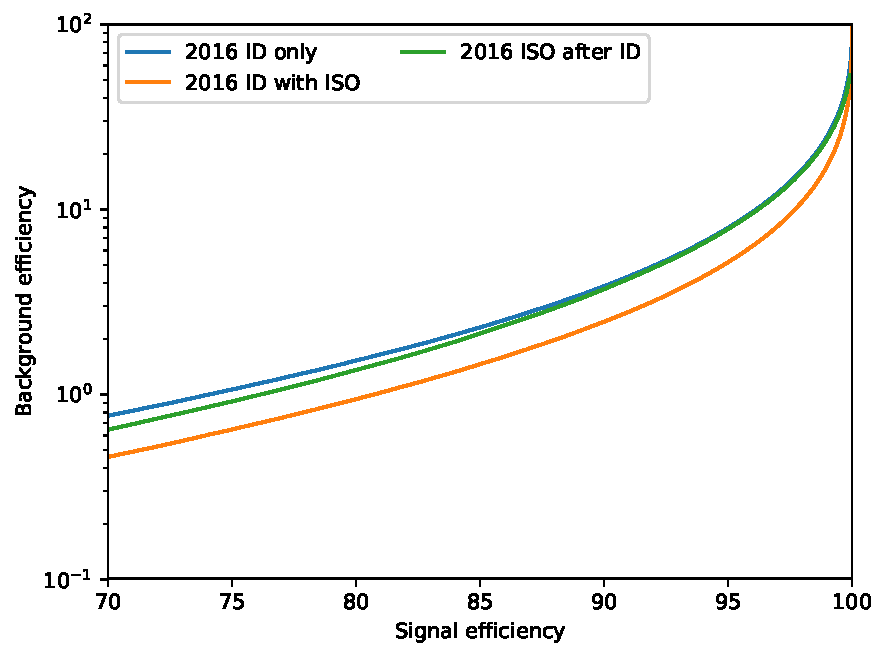
\includegraphics[width=0.45\textwidth]{Figures/Electrons/2016_EE_10_.pdf} \\
   \caption{The receiver operating characteristic curves, representing the background efficiency vs signal efficiency, of the MVA trained on 2016 Drell-Yan with
   jets MC sample. Performance are shown for electrons with $5 < p_T < 10 $ GeV (left), $p_T > 10$ GeV (right), and $|\eta| < 0.8$ (top),
   $0.8 < |\eta| < 1.479$ (middle), and $|\eta| > 1.479$ (bottom).
   \label{fig:ele_ID_ISO_ROC_2016_}}
   \end{center}
\end{figure}

The Fig.~\ref{fig:ele_MVA_score_2018} shows output of the multiclassifier discriminant i.e. MVA score for prompt electrons from Drell-Yan events and
misidentified electrons originating from jets in Drell-Yan events. The performance of  model trained on 2018 MC using electron identification and isolation
features outperforms the model obtained after applying 2017 ID+ISO V2 training on 2018 Drell-Yan with jets MC sample as shown in Fig.~\ref{fig:ele_ID_ISO_ROC_2018}.

\begin{figure}[!htb]
   \vspace*{0.3cm}
   \begin{center}
      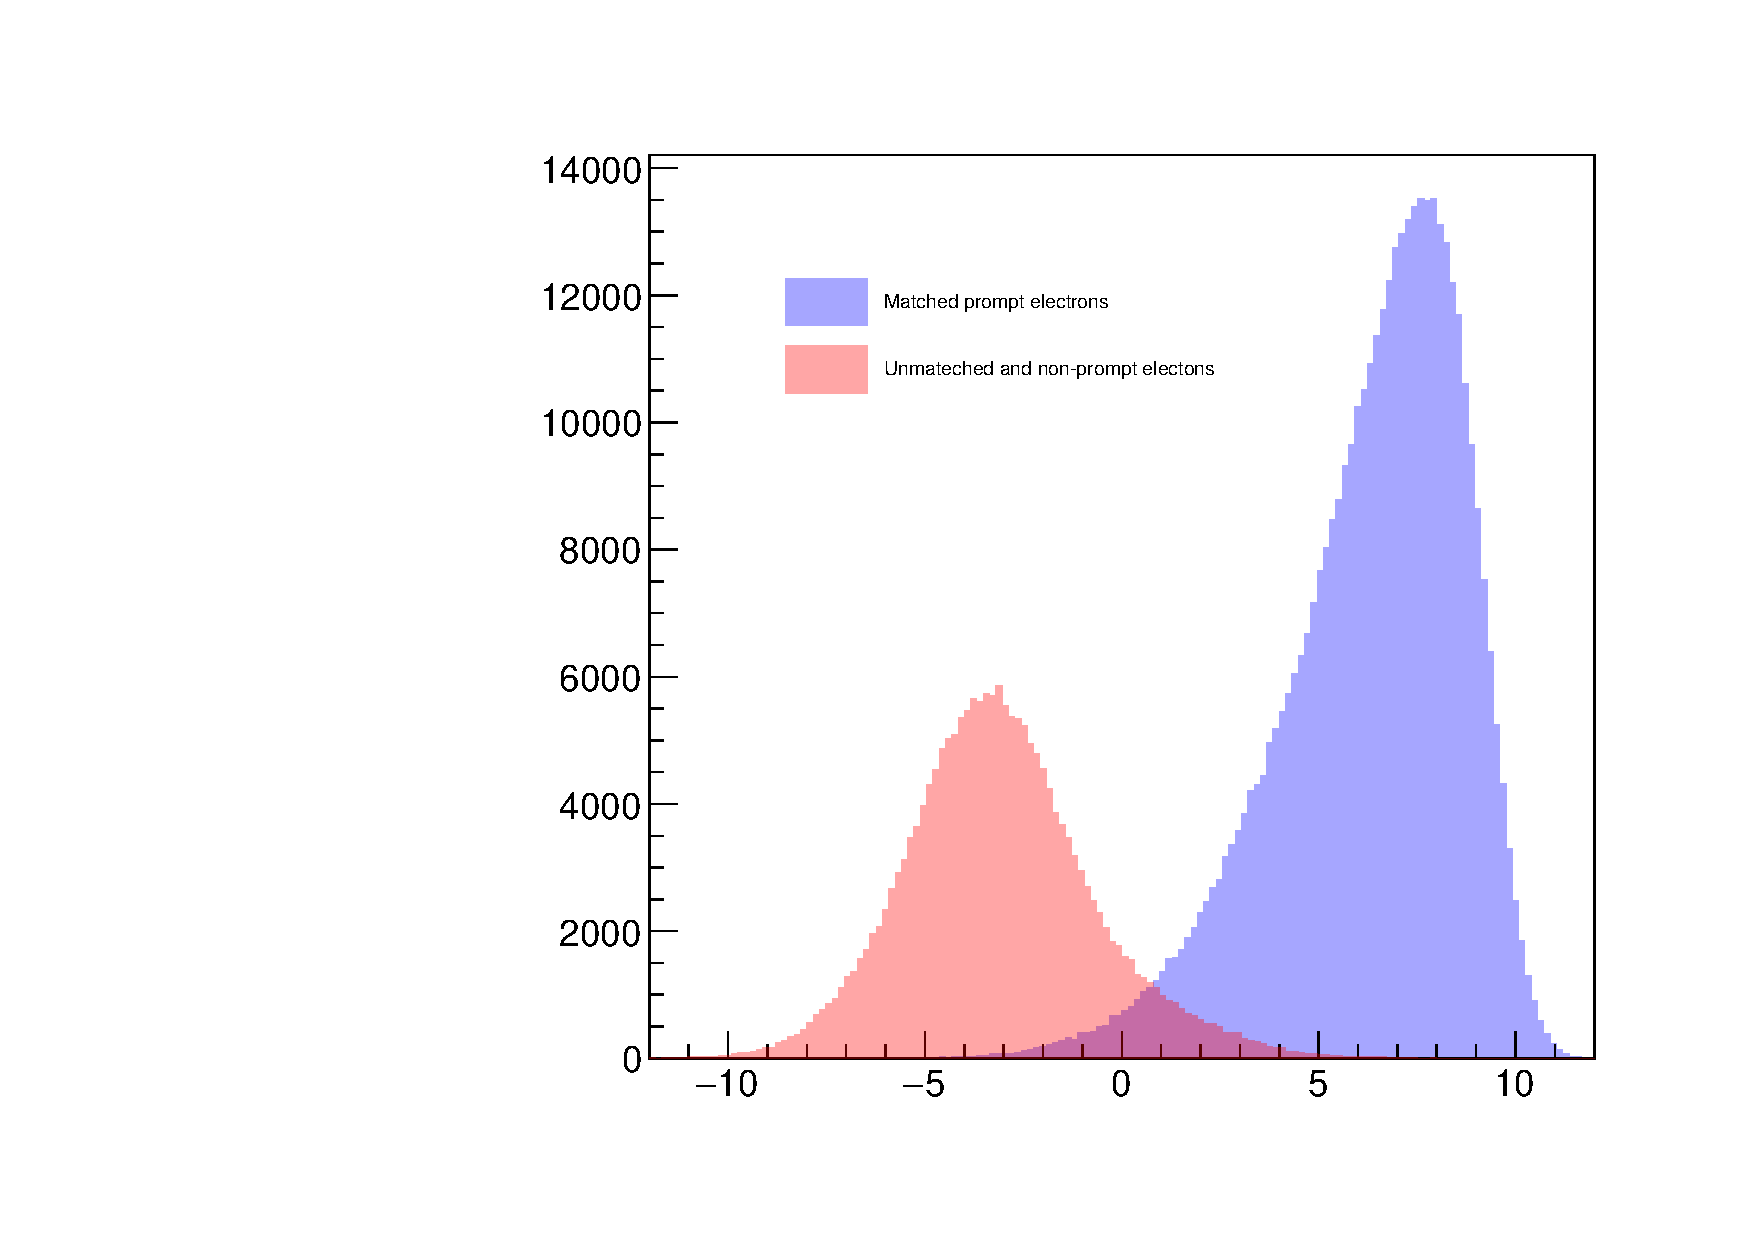
\includegraphics[width=0.80\textwidth]{Figures/Electrons/Ele_BDTv2_Score.pdf}
      \caption{The Output of the multiclassifier discriminant for prompt electrons matched to truth electrons from $Z$ decay (blue) and for misindentified
      electrons (red). Events are all taken from Drell-Yan with jets MC sample.
      \label{fig:ele_MVA_score_2018}}
   \end{center}
\end{figure}

\begin{figure}[!htb]
   \vspace*{0.3cm}
   \begin{center}
      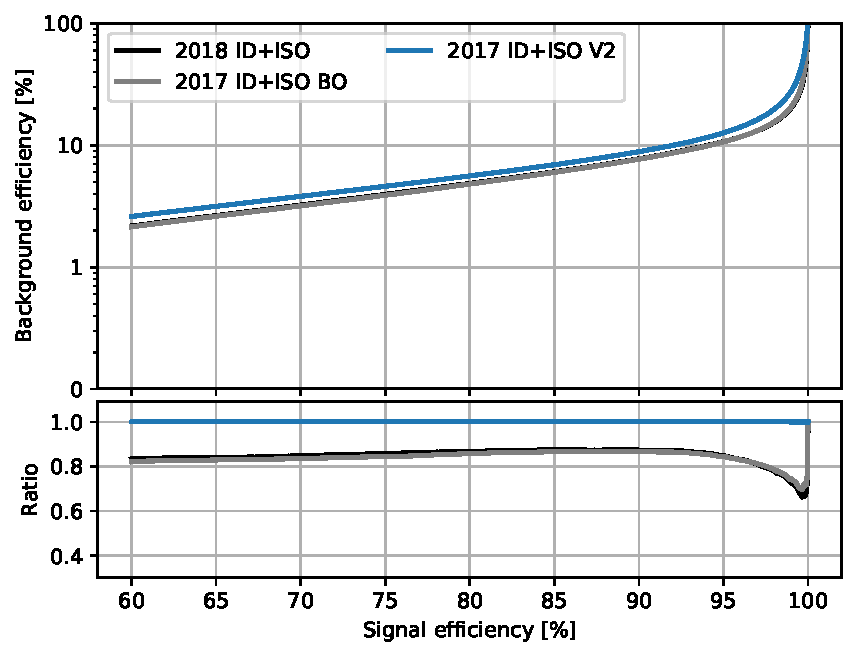
\includegraphics[width=0.45\textwidth]{Figures/Electrons/2018_EB1_5.pdf}
      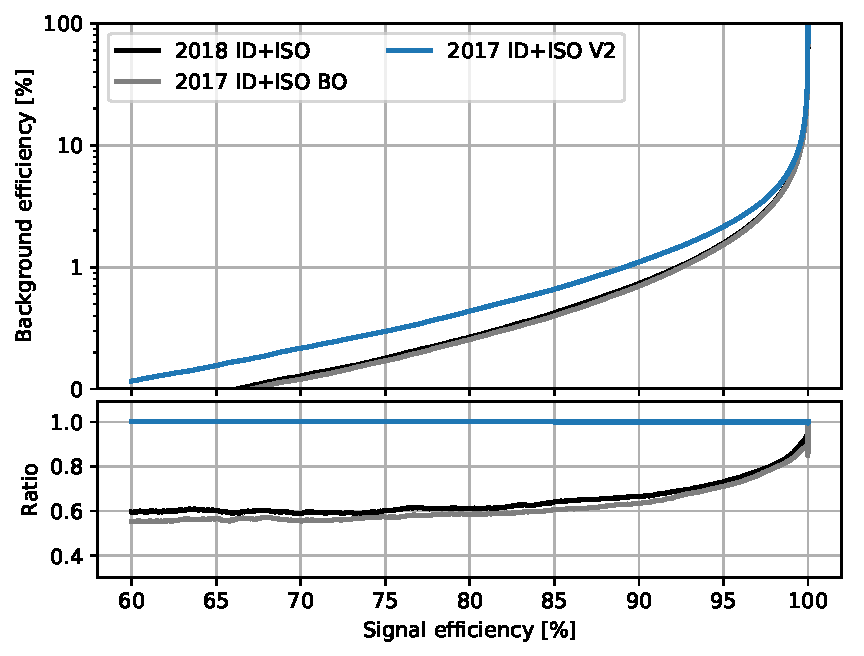
\includegraphics[width=0.45\textwidth]{Figures/Electrons/2018_EB1_10.pdf} \\
      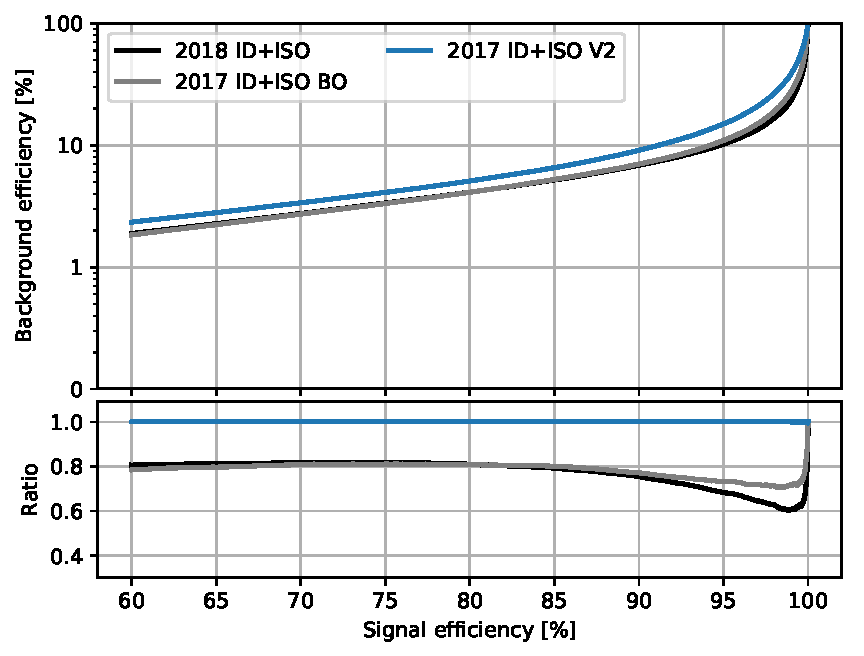
\includegraphics[width=0.45\textwidth]{Figures/Electrons/2018_EB2_5.pdf}
      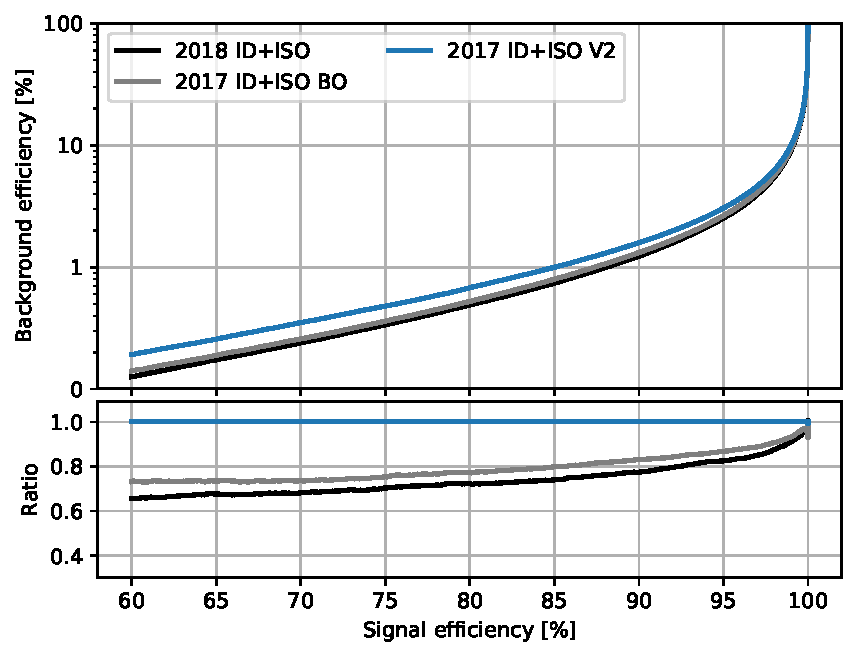
\includegraphics[width=0.45\textwidth]{Figures/Electrons/2018_EB2_10.pdf}\\
      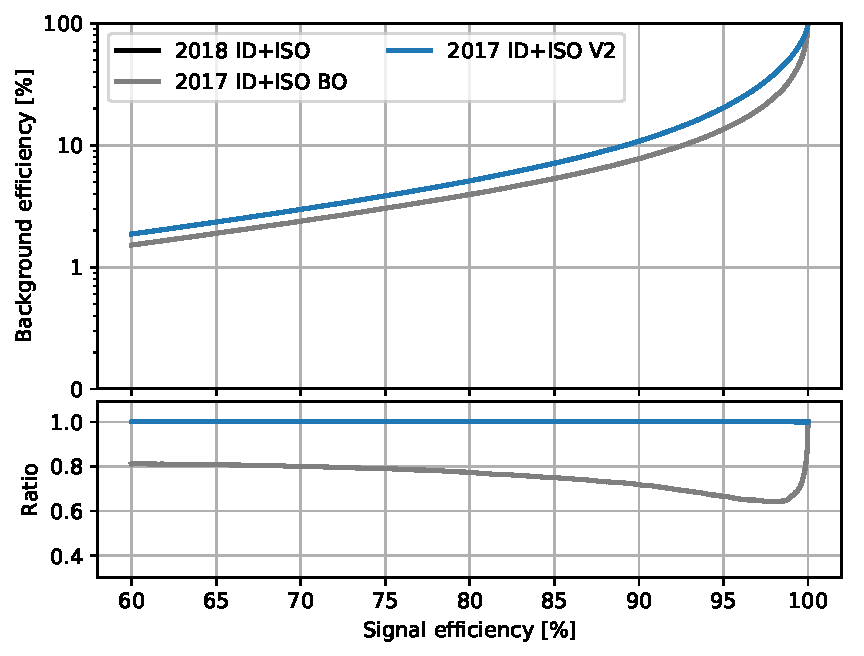
\includegraphics[width=0.45\textwidth]{Figures/Electrons/2018_EE_5.pdf}
      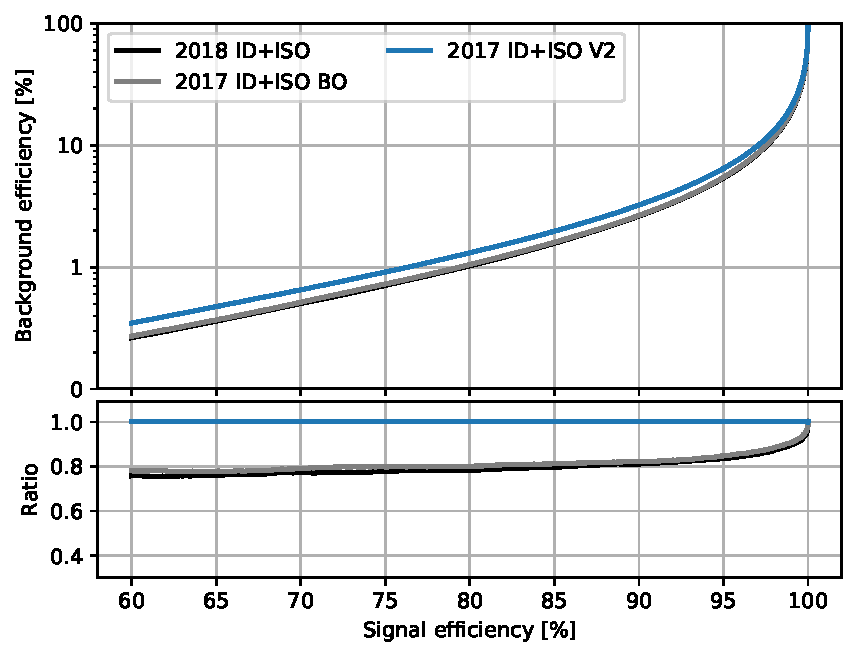
\includegraphics[width=0.45\textwidth]{Figures/Electrons/2018_EE_10.pdf} \\
   \caption{The receiver operating characteristic curves, representing the background efficiency vs signal efficiency, of the MVA trained on the 2017 Drell-Yan
   with jets MC sample and applied on the 2018 Drell-Yan with jets MC sample. The training combines identification and isolation fautures. Performance are shown
   for electrons with $5 < p_T < 10$ GeV (left), $p_T > 10 GeV$ (right), and $|\eta|<0.8$ (top), $0.8 < |\eta| < 1.479$ (middle), and $|\eta| > 1.479$ (bottom).
   V1 and V2 versions of training are compared, exploiting TMVA and xgboost training libraries respectively.
   \label{fig:ele_ID_ISO_ROC_2018}}
   \end{center}
\end{figure}

The impact of the transition from the TMVA (V1) to the XGBoost(V2) training framework is shown in Fig.~\ref{fig:ele_ID_ISO_ROC_V1_vs_V2}, showing a noticeable improvement.
% The working points shown are chosen so as to get the  same signal efficiency as a cut on MVA ID and a cut on the PF isolation, in each $p_T$ and $\eta$ bin.

\begin{figure}[!htb]
   \vspace*{0.3cm}
   \begin{center}
      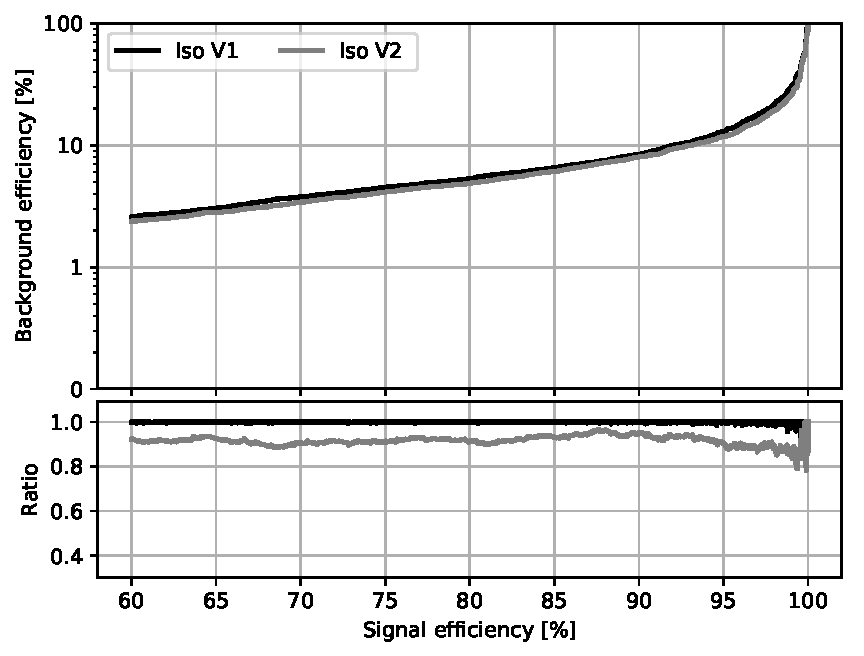
\includegraphics[width=0.45\textwidth]{Figures/Electrons/2018_EB1_5_.pdf}
      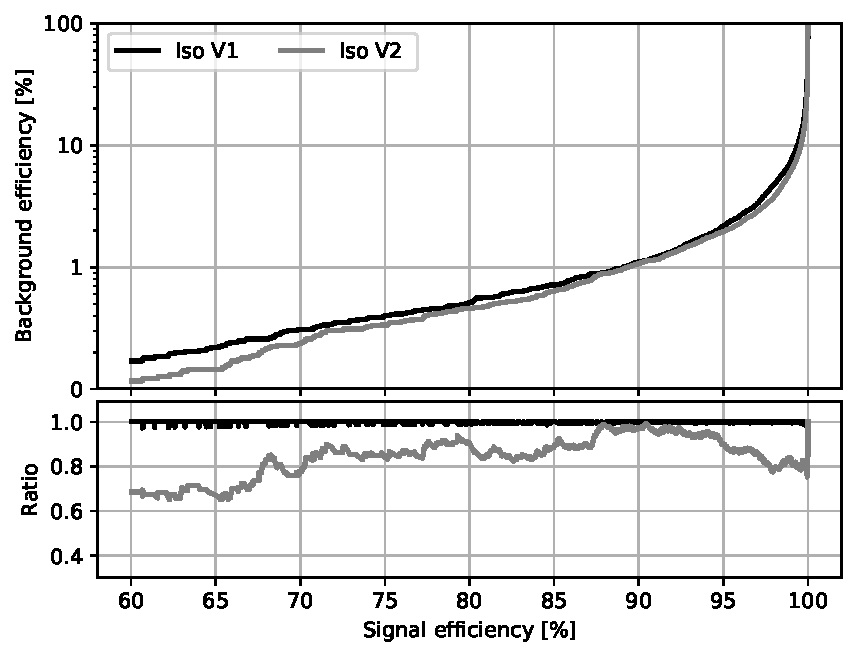
\includegraphics[width=0.45\textwidth]{Figures/Electrons/2018_EB1_10_.pdf} \\
      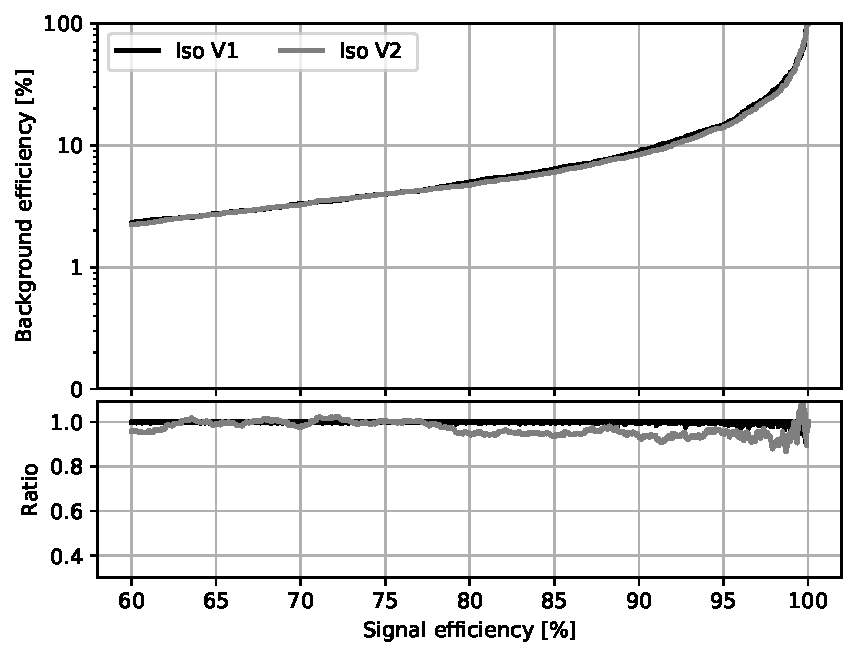
\includegraphics[width=0.45\textwidth]{Figures/Electrons/2018_EB2_5_.pdf}
      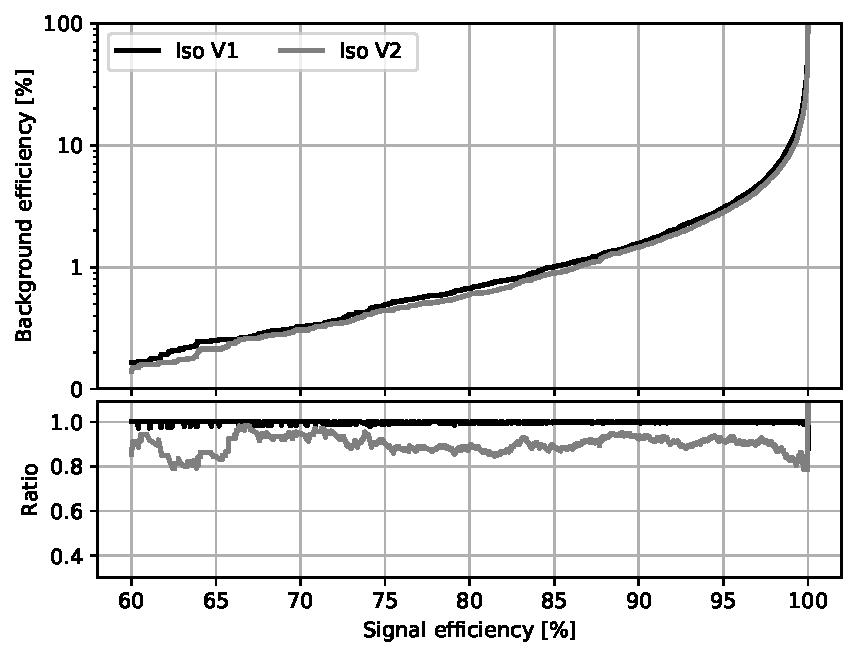
\includegraphics[width=0.45\textwidth]{Figures/Electrons/2018_EB2_10_.pdf} \\
      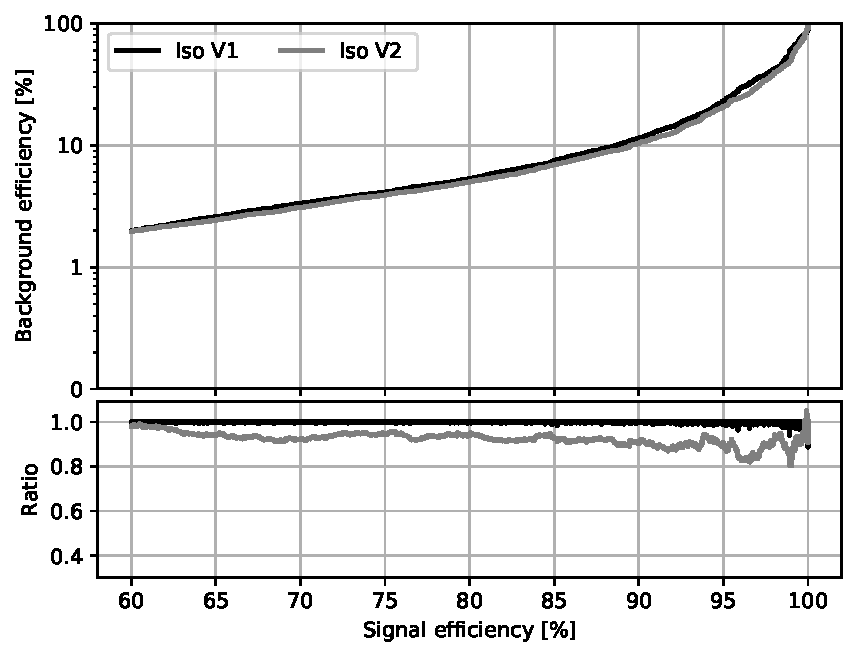
\includegraphics[width=0.45\textwidth]{Figures/Electrons/2018_EE_5_.pdf}
      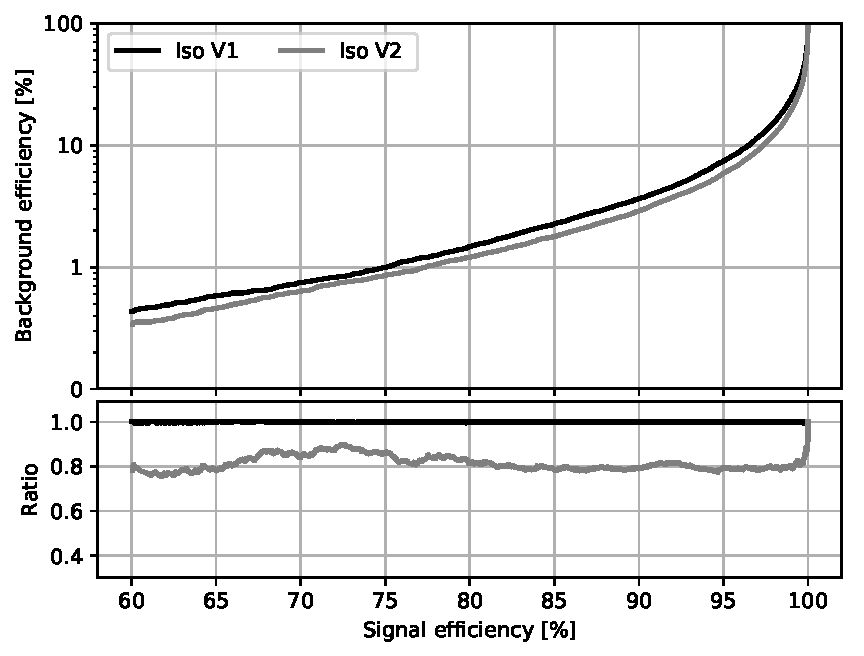
\includegraphics[width=0.45\textwidth]{Figures/Electrons/2018_EE_10_.pdf} \\
   \caption{Performance comparison, background efficiency vs signal efficiency, of the MVA trained using TMVA framework (V1) and XGBoost framework (V2). The
   performance are shown for electrons with $5 < p_T < 10$ GeV (left), $p_T > 10 GeV$ (right), and $|\eta|<0.8$ (top), $0.8 < |\eta| < 1.479$ (middle), and
   $|\eta| > 1.479$ (bottom).
\label{fig:ele_ID_ISO_ROC_V1_vs_V2}}
\end{center}
\end{figure}



% \begin{figure}[!htb]
% \vspace*{0.3cm}
% \begin{center}
% \includegraphics[width=0.5\textwidth]{Figures/Electrons/ele_overtraining.png}
% \caption{BDT output for the training and testing sample for true and fake electrons in the high-$p_T$ endcap training bins.
% \label{fig:ele_ID_BDT_output}}
% \end{center}
% \end{figure}

%Table~\ref{tab:ele_ID_input_variables} summarizes the full list of observables used as input to the classifier
Tables~\ref{tab:ele_ID_WPA},~\ref{tab:ele_ID_WPB} and ~\ref{tab:ele_ID_WPC} list the cuts values applied to the MVA output for 2016, 2017, 2018 training, respectively. For 2018, the corresponding signal and background efficiencies are given as examples.They are very similar for 2016 and 2017. 
%e for the chosen working point. 
For the analysis, loose electrons have to pass this MVA identification and isolation working point.

\begin{table}[h!]
%\scriptsize
    \centering
    \begin{tabular}{c|c c c}
\hline
\multicolumn{4}{|c|}{2016 Datasets}                                                                 \\
\hline %----------------------------------------------------------------------------------------
minimum BDT score    &  $|\eta| < 0.8 $ & $0.8 < |\eta| < 1.479$ 	& $|\eta| > 1.479$      \\
\hline %----------------------------------------------------------------------------------------
$ 5 < p_T < 10 $ GeV &  0.9503      & 0.9461  	& 0.9387		\\
$p_T > 10$ GeV         &  0.3782	& 0.3587		&  -0.5745	\\
\hline %----------------------------------------------------------------------------------------
\hline %----------------------------------------------------------------------------------------
     \end{tabular}
\small
    \caption{Minimum BDT score required for passing the electron identification, for 2016 samples.}% \textbf{FIXME: WP to be defined!}}
    \label{tab:ele_ID_WPA}
\end{table}

\begin{table}[h!]
%\scriptsize
    \centering
    \begin{tabular}{c|c c c}
\hline
\multicolumn{4}{|c|}{2017 Datasets}                                                                 \\
\hline %----------------------------------------------------------------------------------------
minimum BDT score    &  $|\eta| < 0.8 $ & $0.8 < |\eta| < 1.479$ 	& $|\eta| > 1.479$      \\
\hline %----------------------------------------------------------------------------------------
$ 5 < p_T < 10 $ GeV &  0.8521    & 0.8268  	& 0.8694		\\
$p_T > 10$ GeV         &  0.9825    & 0.9692	& 0.7935	\\
\hline %----------------------------------------------------------------------------------------
\hline %----------------------------------------------------------------------------------------
     \end{tabular}
\small
    \caption{Minimum BDT score required for passing the electron identification, for 2017 samples.}% \textbf{FIXME: WP to be defined!}}
    \label{tab:ele_ID_WPB}
\end{table}

%2016
 %= (pt<=10 && ((fSCeta<0.8                  && BDT >  0.95034841889) ||
 %                                 (fSCeta>=0.8 && fSCeta<1.479 && BDT >  0.94606270058) ||
 %                                (fSCeta>=1.479               && BDT >  0.93872558098)))
 %                   || (pt>10  && ((fSCeta<0.8                  && BDT >  0.3782357877) ||
   %                                (fSCeta>=0.8 && fSCeta<1.479 && BDT >  0.35871320305) ||
      %                             (fSCeta>=1.479               && BDT >  -0.57451499543)));

%2017
 %  isBDT         = (pt<=10 && ((fSCeta<0.8                  && BDT >  0.85216885148) ||
   %                                (fSCeta>=0.8 && fSCeta<1.479 && BDT >  0.82684550976) ||
   %                                (fSCeta>=1.479               && BDT >  0.86937630022)))
     %               || (pt>10  && ((fSCeta<0.8                  && BDT >  0.98248928759) ||
    %                               (fSCeta>=0.8 && fSCeta<1.479 && BDT >  0.96919224579) ||
   %                                (fSCeta>=1.479               && BDT >  0.79349796445)));

\begin{table}[h!]
%\scriptsize
    \centering
    \begin{tabular}{|c|c c c}
%\multicolumn{4}{|c|}{Datasets}                                                                 \\
%\hline %----------------------------------------------------------------------------------------
\cline{2-4}
  \multicolumn{1}{ c|}{}             & \multicolumn{3}{|c|}{$|\eta| < 0.8 $}                        \\
\cline{2-4} %----------------------------------------------------------------------------------------
   \multicolumn{1}{c|}{}            & Cut on BDT score & Signal eff. & \multicolumn{1}{c|}{Background eff.}  \\
\hline %----------------------------------------------------------------------------------------
$ 5 < p_T < 10 $ GeV              & 0.8956                        & 81.04\%            &  \multicolumn{1}{c|}{4.4\%}  \\
\hline %----------------------------------------------------------------------------------------
 $p_T > 10$ GeV                     &  0.0424	           	     & 97.1\%		&  \multicolumn{1}{c|}{2.9\%}		\\
\hline %----------------------------------------------------------------------------------------
\cline{2-4}
  \multicolumn{1}{ c|}{}             & \multicolumn{3}{|c|}{$0.8 < |\eta| < 1.479$}                        \\
\cline{2-4} %----------------------------------------------------------------------------------------
   \multicolumn{1}{c|}{}            & Cut on BDT score & Signal eff.      & \multicolumn{1}{c|}{Background eff.}  \\
\hline  %----------------------------------------------------------------------------------------
$ 5 < p_T < 10 $ GeV              & 0.9111                     & 79.3\%           &  \multicolumn{1}{c|}{4.6\%}     \\
\hline %----------------------------------------------------------------------------------------
$p_T > 10$ GeV                      &  0.0047		         & 96.3\%	  &  \multicolumn{1}{c|}{3.6\%}		\\
\hline %----------------------------------------------------------------------------------------

\cline{2-4}
  \multicolumn{1}{ c|}{}             & \multicolumn{3}{|c|}{$|\eta| > 1.479$}                        \\
\cline{2-4} %----------------------------------------------------------------------------------------
   \multicolumn{1}{c|}{}            & Cut on BDT score & Signal eff. & \multicolumn{1}{c|}{Background eff.}  \\
\hline  %----------------------------------------------------------------------------------------
$ 5 < p_T < 10 $ GeV              & 0.9401                     & 72.97\%    &  \multicolumn{1}{c|}{3.6\%}     \\
\hline %----------------------------------------------------------------------------------------
$p_T > 10$ GeV                      & -0.6042		   & 95.7\%      &  \multicolumn{1}{c|}{6.7\%}		\\
\hline %----------------------------------------------------------------------------------------

     \end{tabular}
\small
    \caption{Minimum MVA score required for passing the electron identification, together with the corresponding signal and background efficiencies, for 2018 samples.}
\label{tab:ele_ID_WPC}
\end{table}

\clearpage

%
%\subsubsection{Electron Impact Parameter Selection}
%\label{sec:eleSIP}
% In order to ensure that the leptons are consistent with a common primary vertex we require that they have an associated track with a small impact parameter with respect to the event primary vertex.  
We use the significance of the impact parameter to the event vertex, $  {\rm SIP_{3D}} = \frac{\rm IP}{\sigma_{\rm IP}} $, where ${\rm IP}$ is the lepton impact parameter in three dimensions at the point of closest approach with respect to the primary interaction vertex, and $\sigma_{\rm IP}$ the associated uncertainty.  Hereafter, a "primary lepton" is a lepton satisfying $| {\rm SIP_{3D}} | < 4$.               

%
\subsubsection{Electron Energy Calibrations}
%\textbf{FIXME: ReRecoed data are used but additional e-scale and smearing corrections NOT yet available and thus NOT yet applied}
Referred to \cite{CMS-PAS-HIG-19-001}.
%Electrons in data are corrected for features in ECAL energy scale
%in bins of $\pt$ and $\left| \eta \right|$. Corrections are calculated
%on a $\cPZ \to \Pe\Pe$ sample to align the dielectron 
%mass spectrum in the data to that in the MC, and to
%minimize its width.
%
%The $\cPZ \to \Pe\Pe$ mass resolution in Monte Carlo is made to match
%data by applying a pseudorandom Gaussian smearing to electron energies,
%with Gaussian parameters varying in bins of $\pt$ and $\left| \eta \right|$.
%This has the effect of convoluting the electron energy spectrum with a
%Gaussian.
%
%The electron energy scale is measured in data by fitting a Crystall-ball function to the di-electron mass spectrum around the Z peak in the $Z\rightarrow \Pe \Pe$ control region. The energy scale for the 2016, 2017 and 2018 dataset are shown in Fig.~\ref{fig:ele_energy_scaleA},~\ref{fig:ele_energy_scaleB},~\ref{fig:ele_energy_scaleC} (a), respectively, and decently agrees with the MC with the preliminary corrections released so far by EGAMMA POG. % for Moriond. % even without any corrections available at the moment. 
%
%\begin{figure}[!htb]
%\vspace*{0.3cm}
%\begin{center}
%\subfigure [] {\resizebox{8cm}{!}{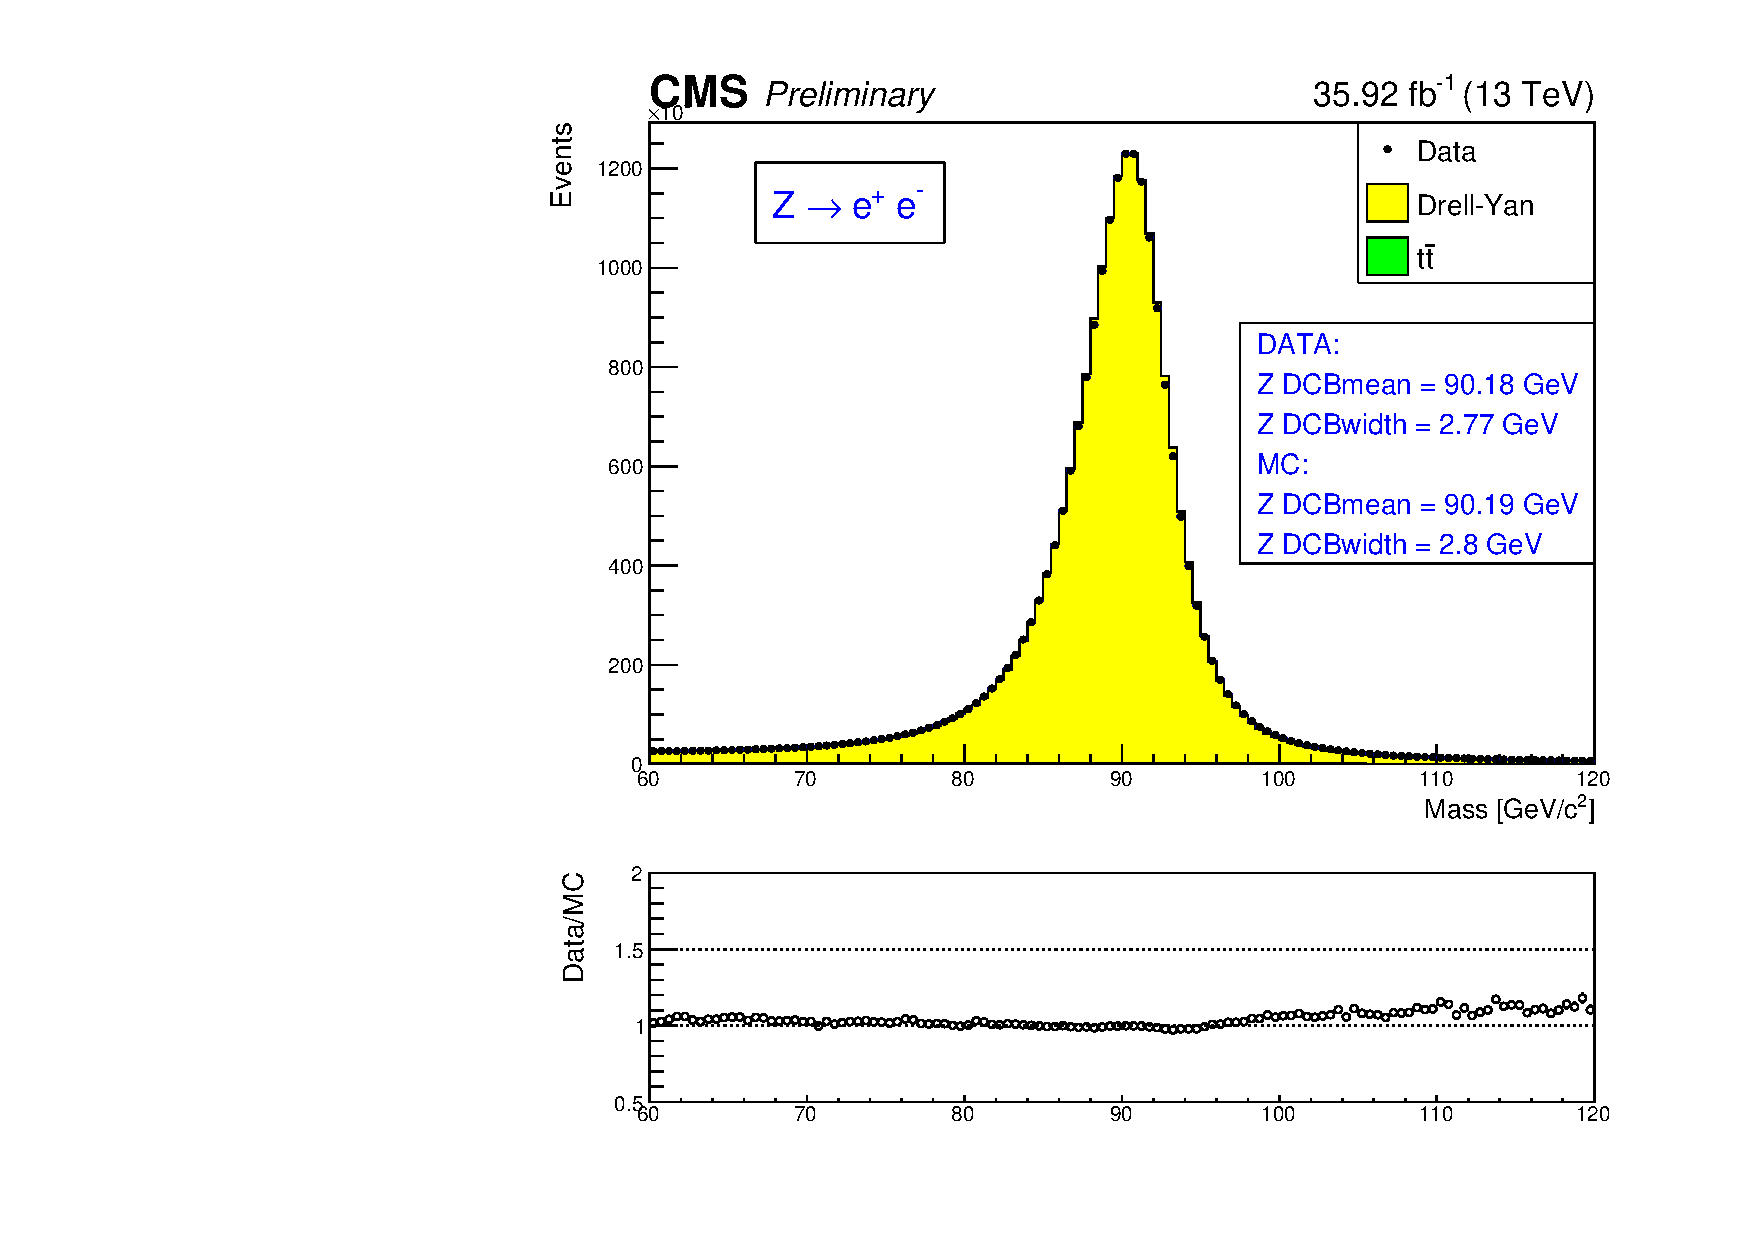
\includegraphics{Figures/Electrons/2016_ZMass_ele.pdf}}}
%\subfigure [] {\resizebox{8cm}{!}{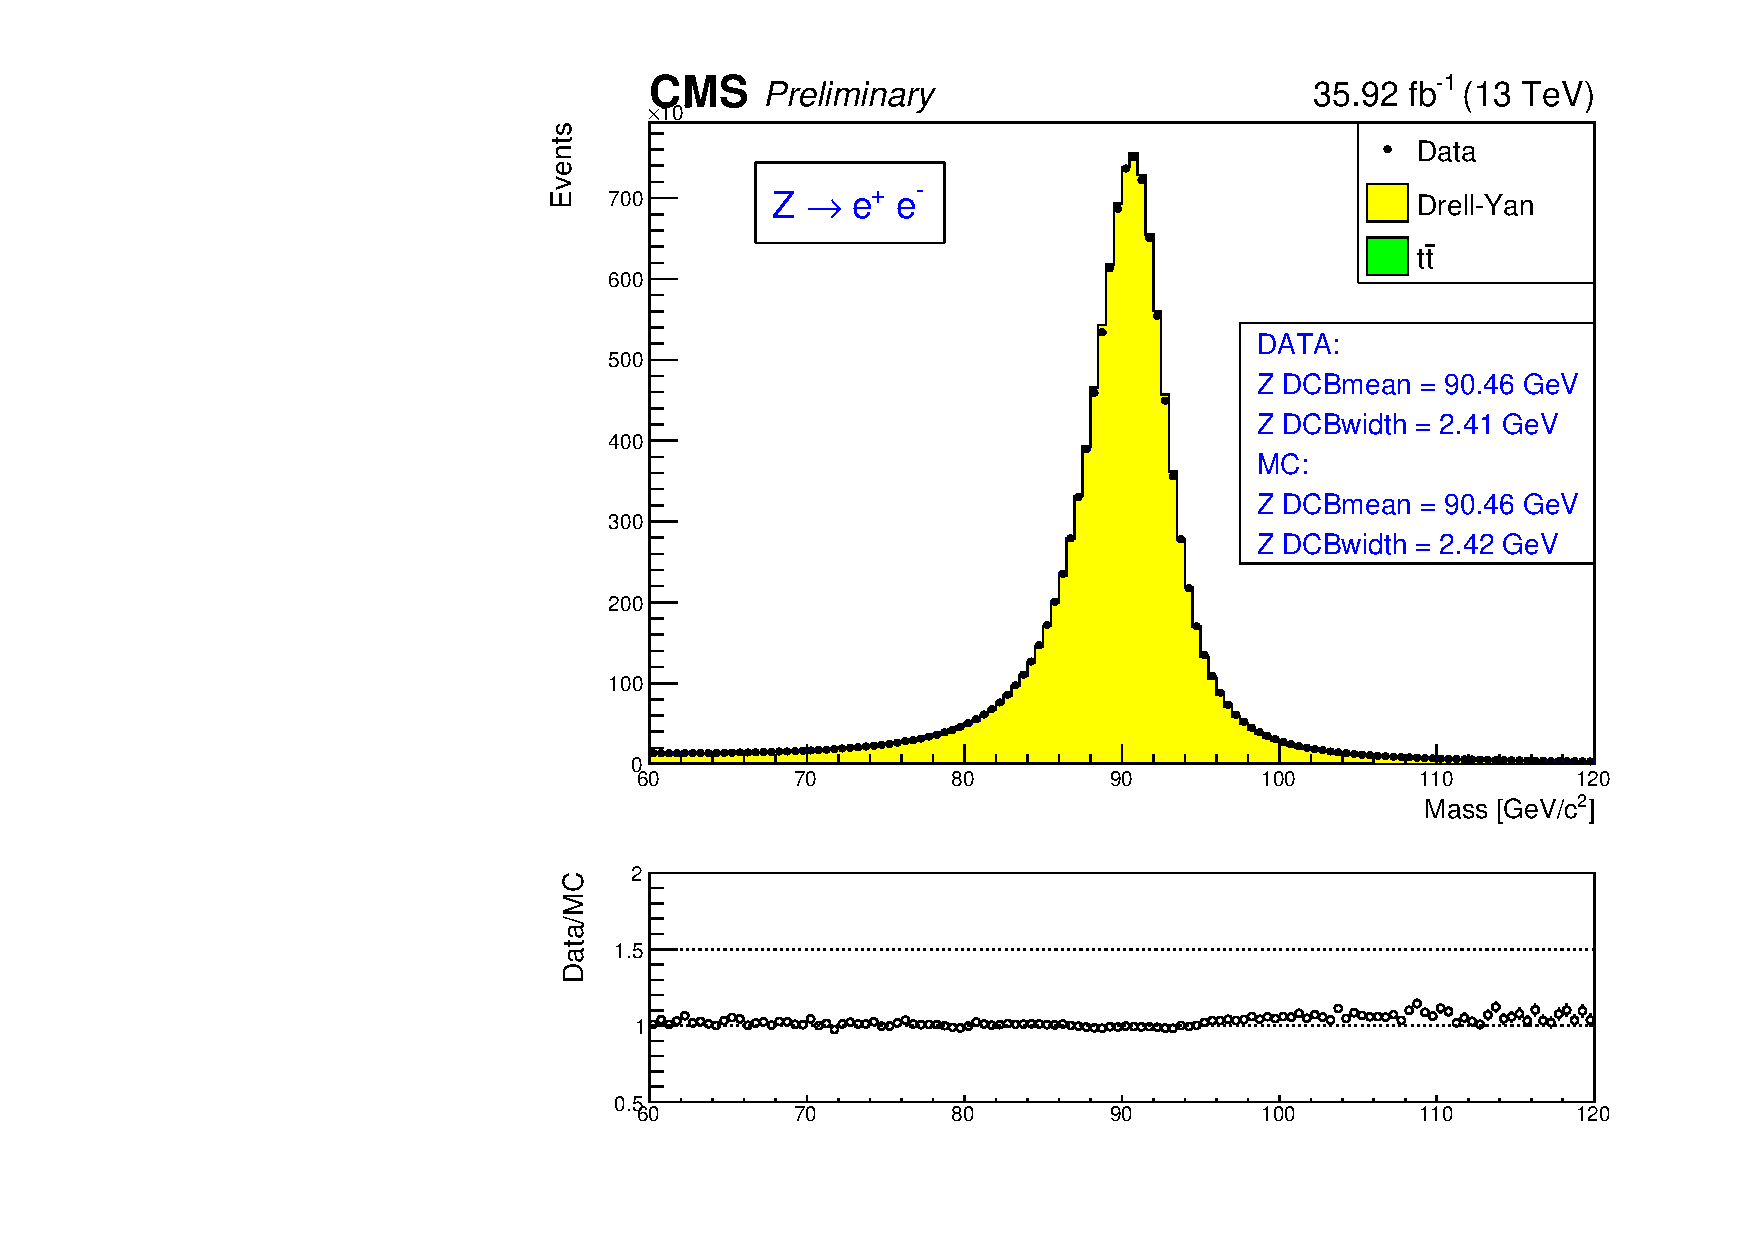
\includegraphics{Figures/Electrons/2016_ZMass_ele_EBEB.pdf}}} \\
%\subfigure [] {\resizebox{8cm}{!}{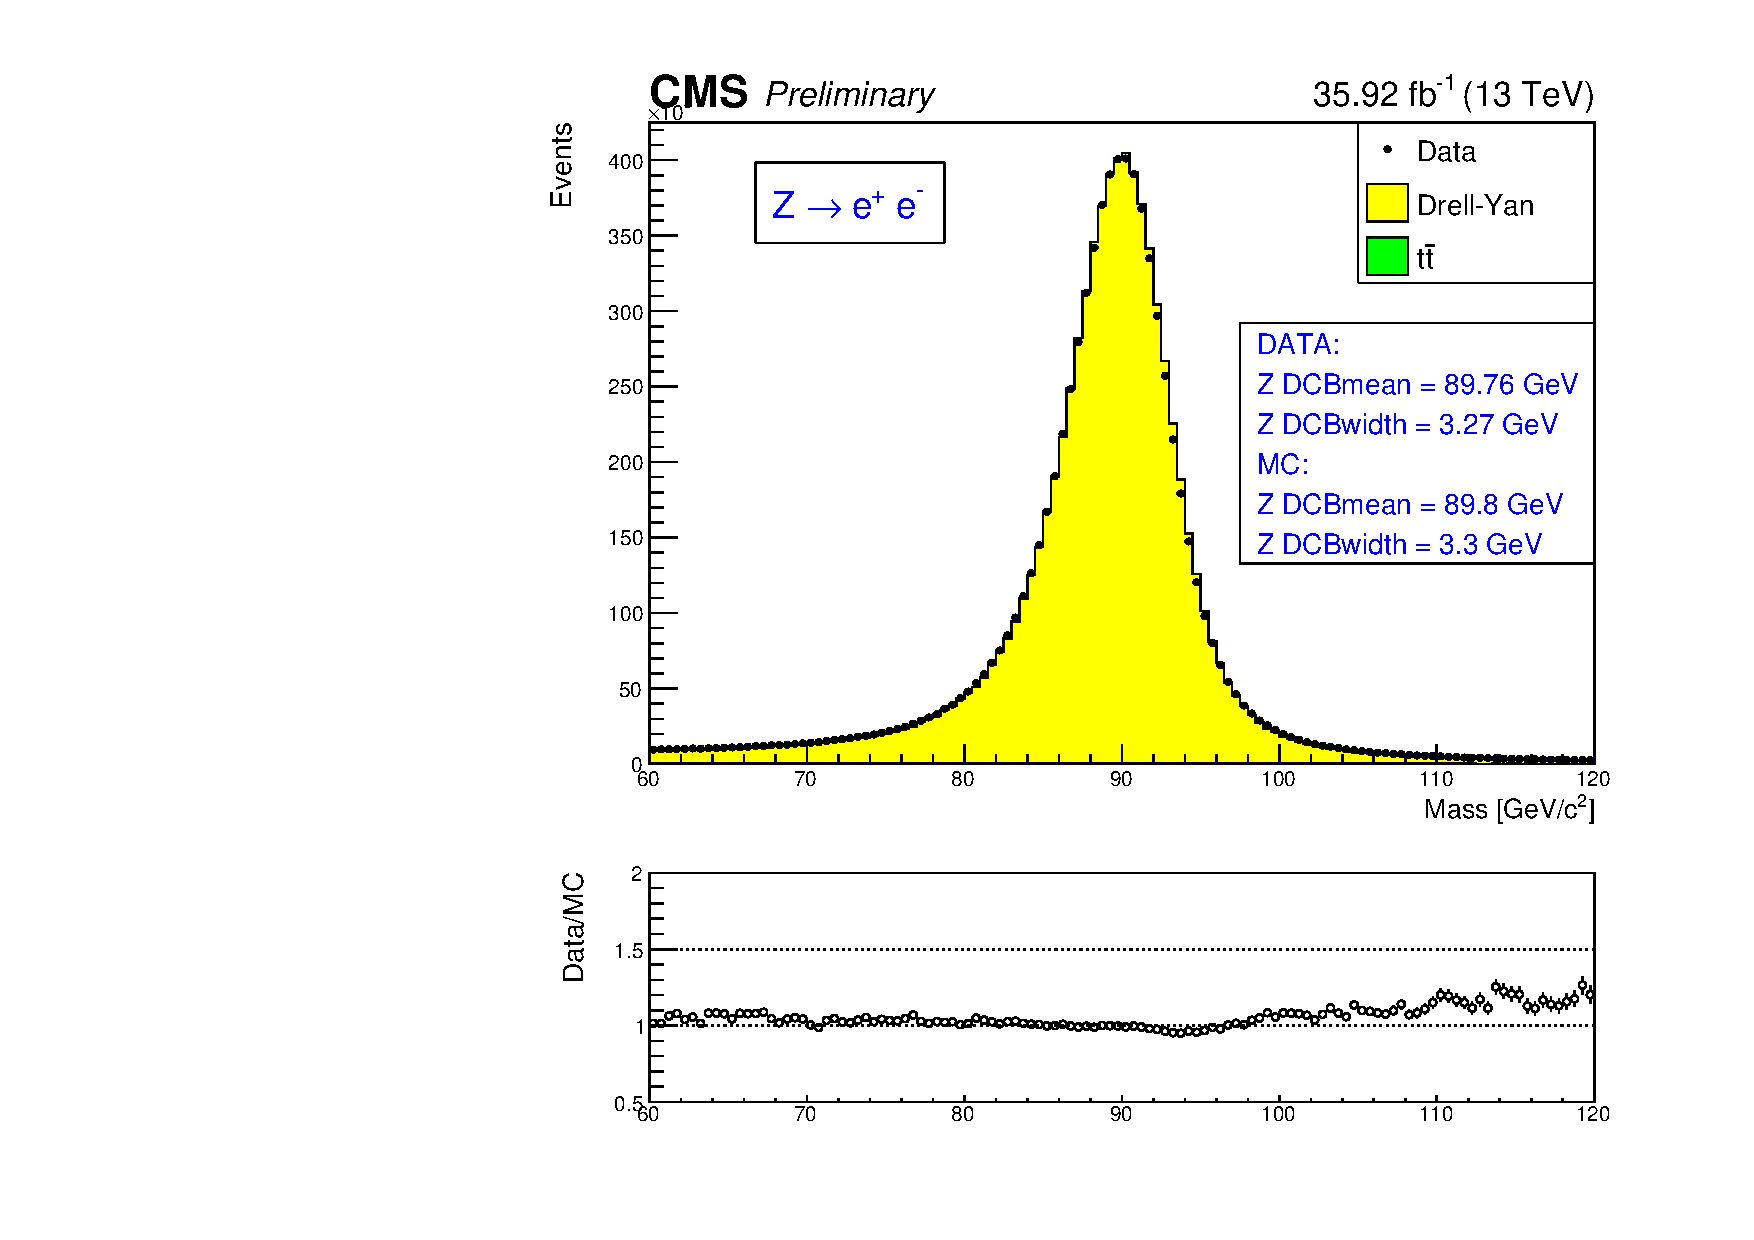
\includegraphics{Figures/Electrons/2016_ZMass_ele_EBEE.pdf}}}
%\subfigure [] {\resizebox{8cm}{!}{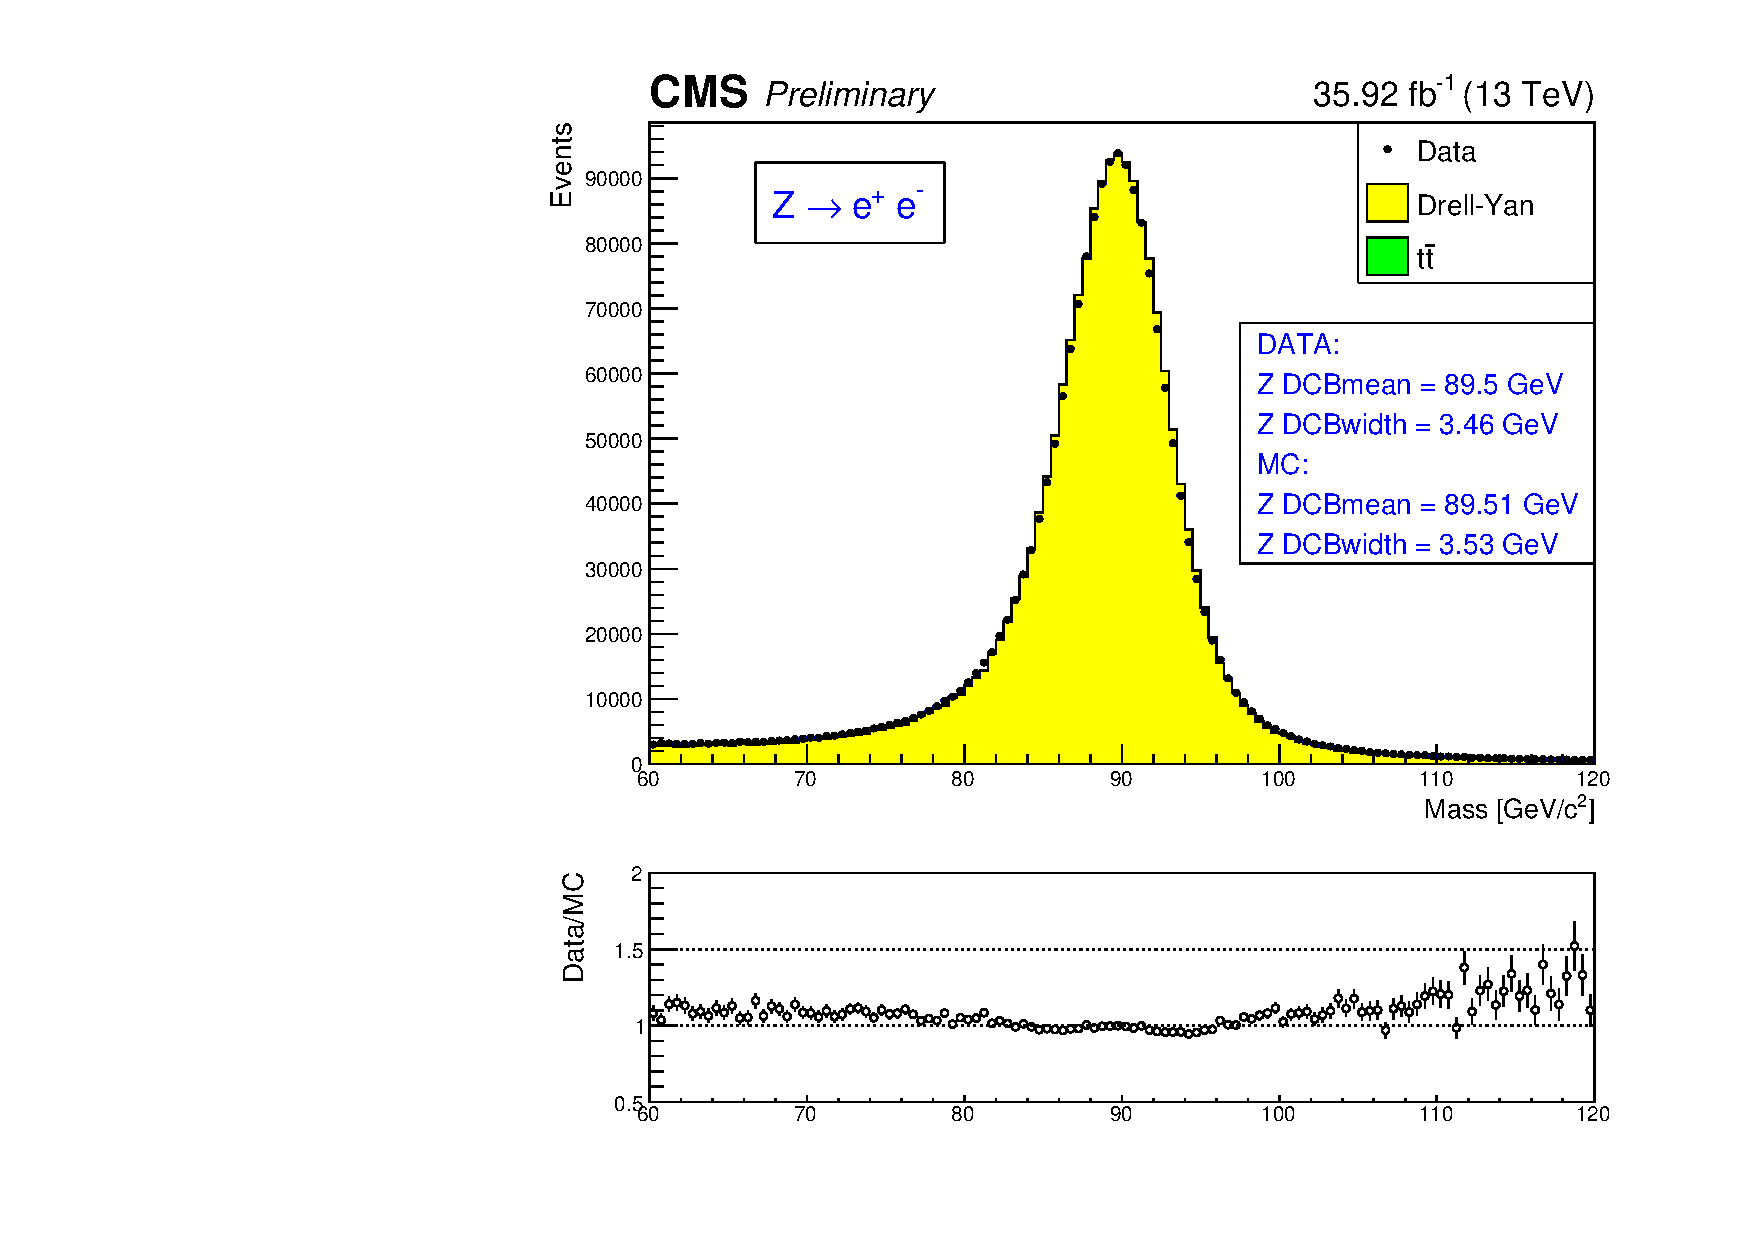
\includegraphics{Figures/Electrons/2016_ZMass_ele_EEEE.pdf}}} \\
%\end{center}
%\caption{
%(a): electron energy scale measured in the $Z\rightarrow \Pe \Pe$ control region for all electrons, for both electrons in the barrel (b), for one electron in the barrel, one in the endcaps (c) and for both electrons in the endcaps (d), for 2016 data.
%The results of the Crystall-ball fit are reported in the figures.
%%\textbf{FIXME: e-scale and smearing corrections NOT yet available and thus NOT yet applied} 
%}
%\label{fig:ele_energy_scaleA}
%\end{figure}
%
%\begin{figure}[!htb]
%\vspace*{0.3cm}
%\begin{center}
%\subfigure [] {\resizebox{8cm}{!}{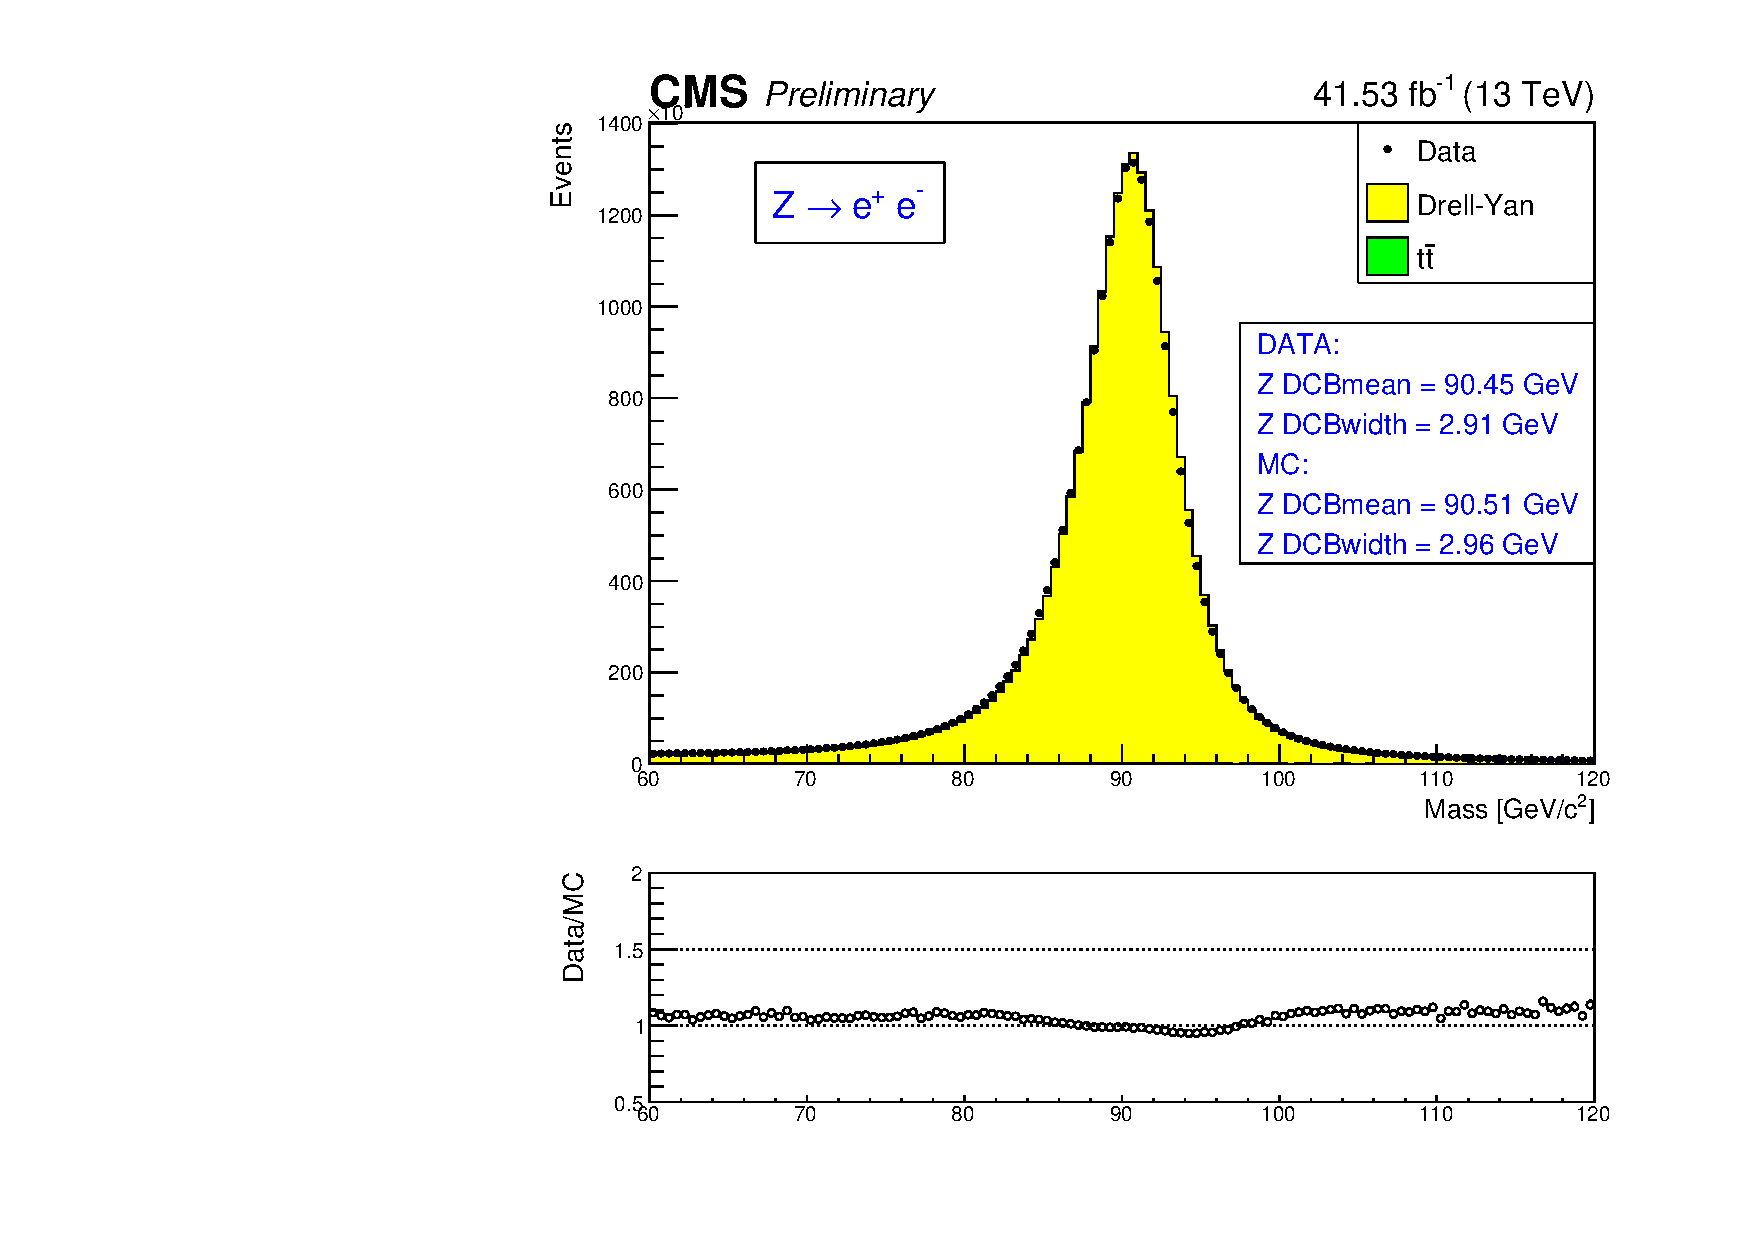
\includegraphics{Figures/Electrons/2017_ZMass_ele.pdf}}}
%\subfigure [] {\resizebox{8cm}{!}{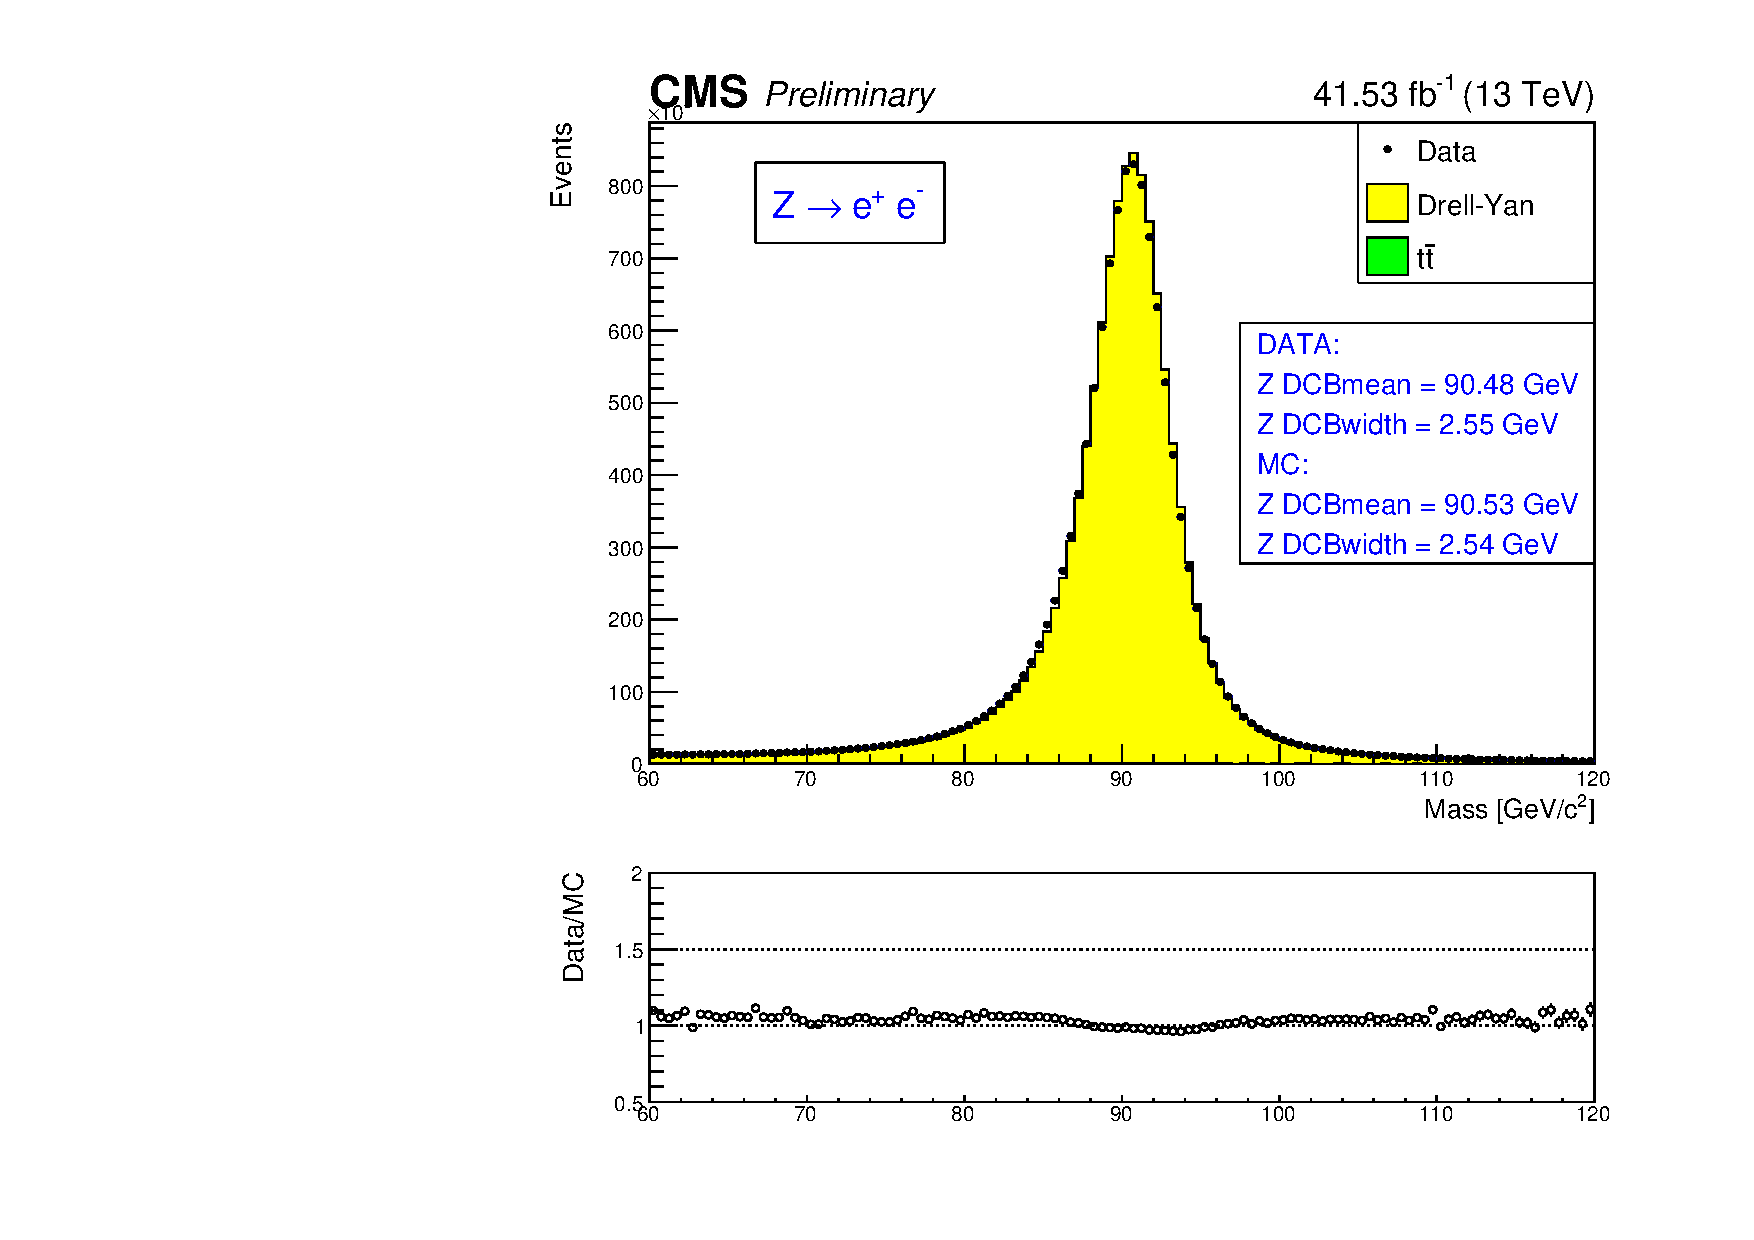
\includegraphics{Figures/Electrons/2017_ZMass_ele_EBEB.pdf}}} \\
%\subfigure [] {\resizebox{8cm}{!}{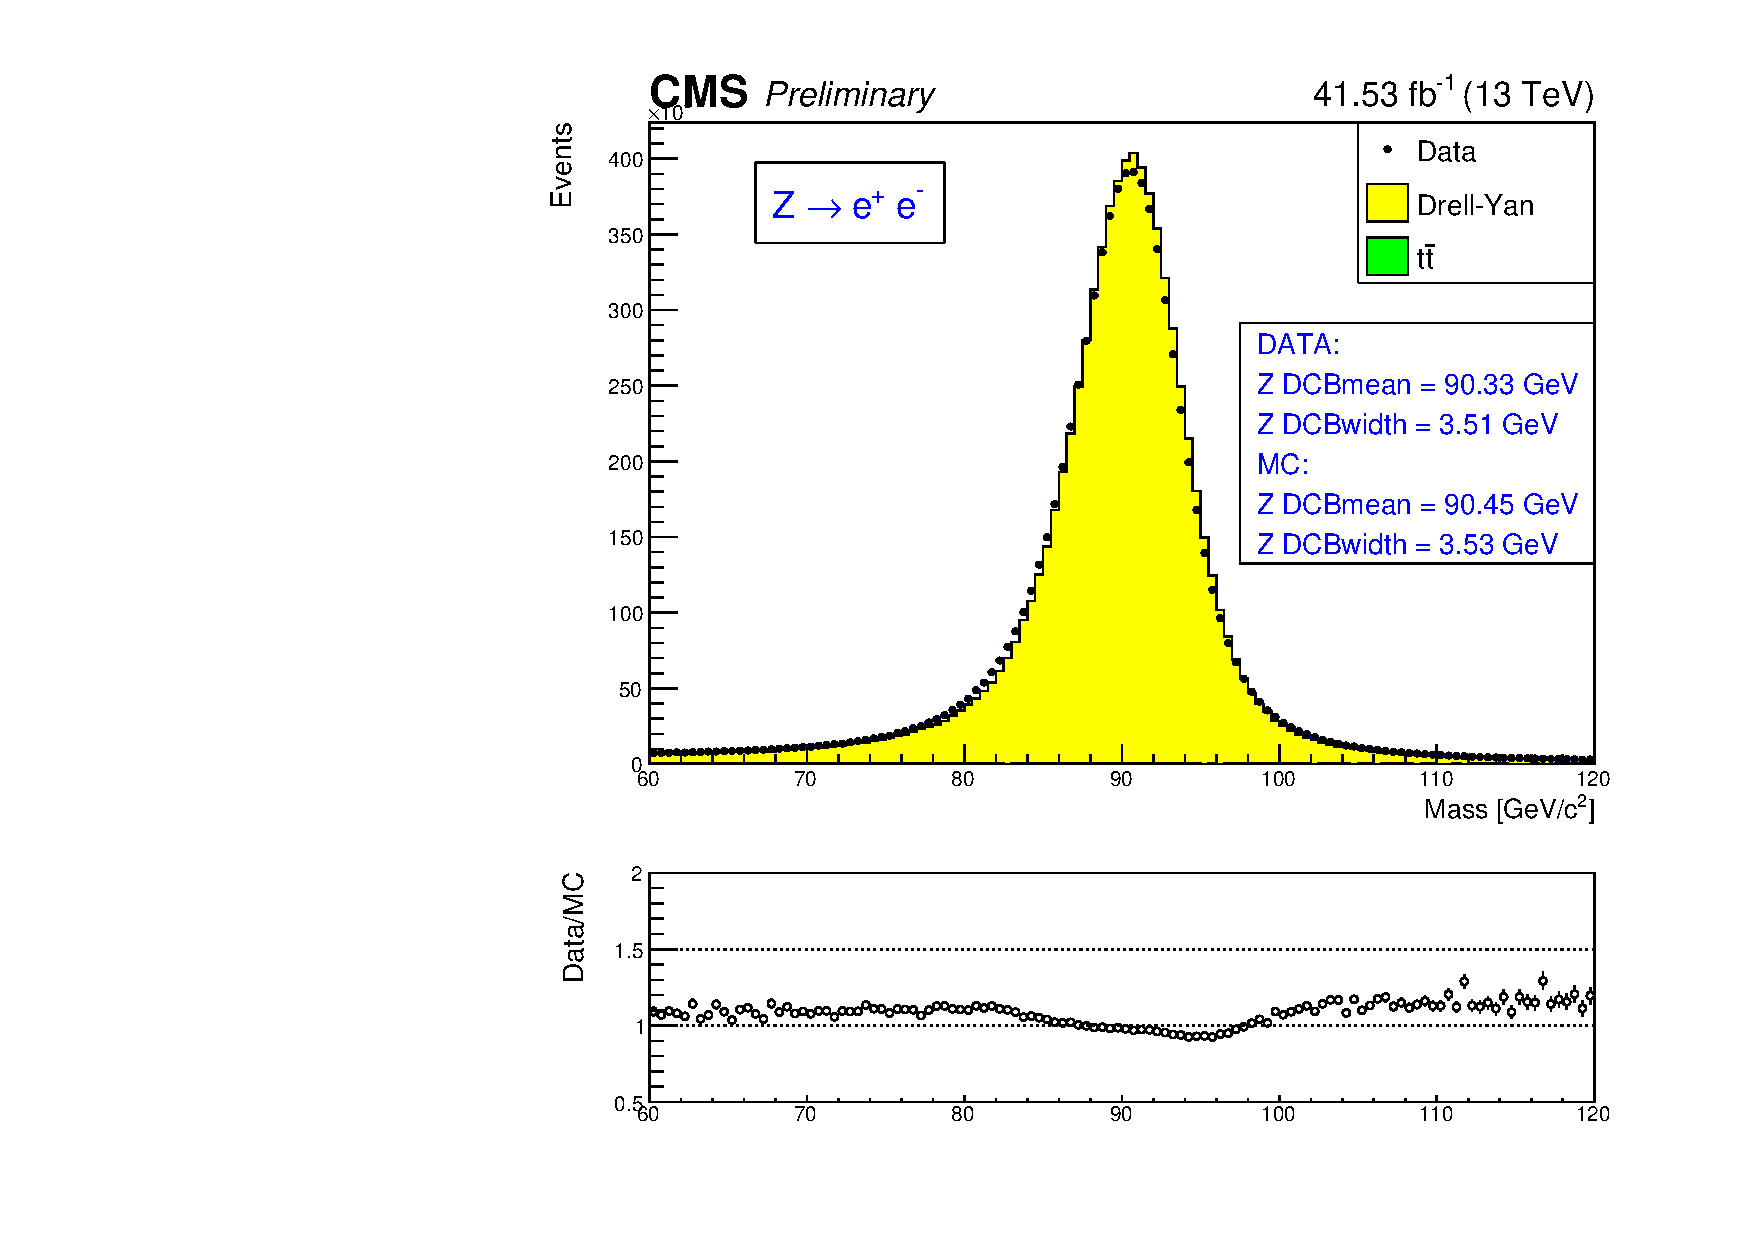
\includegraphics{Figures/Electrons/2017_ZMass_ele_EBEE.pdf}}}
%\subfigure [] {\resizebox{8cm}{!}{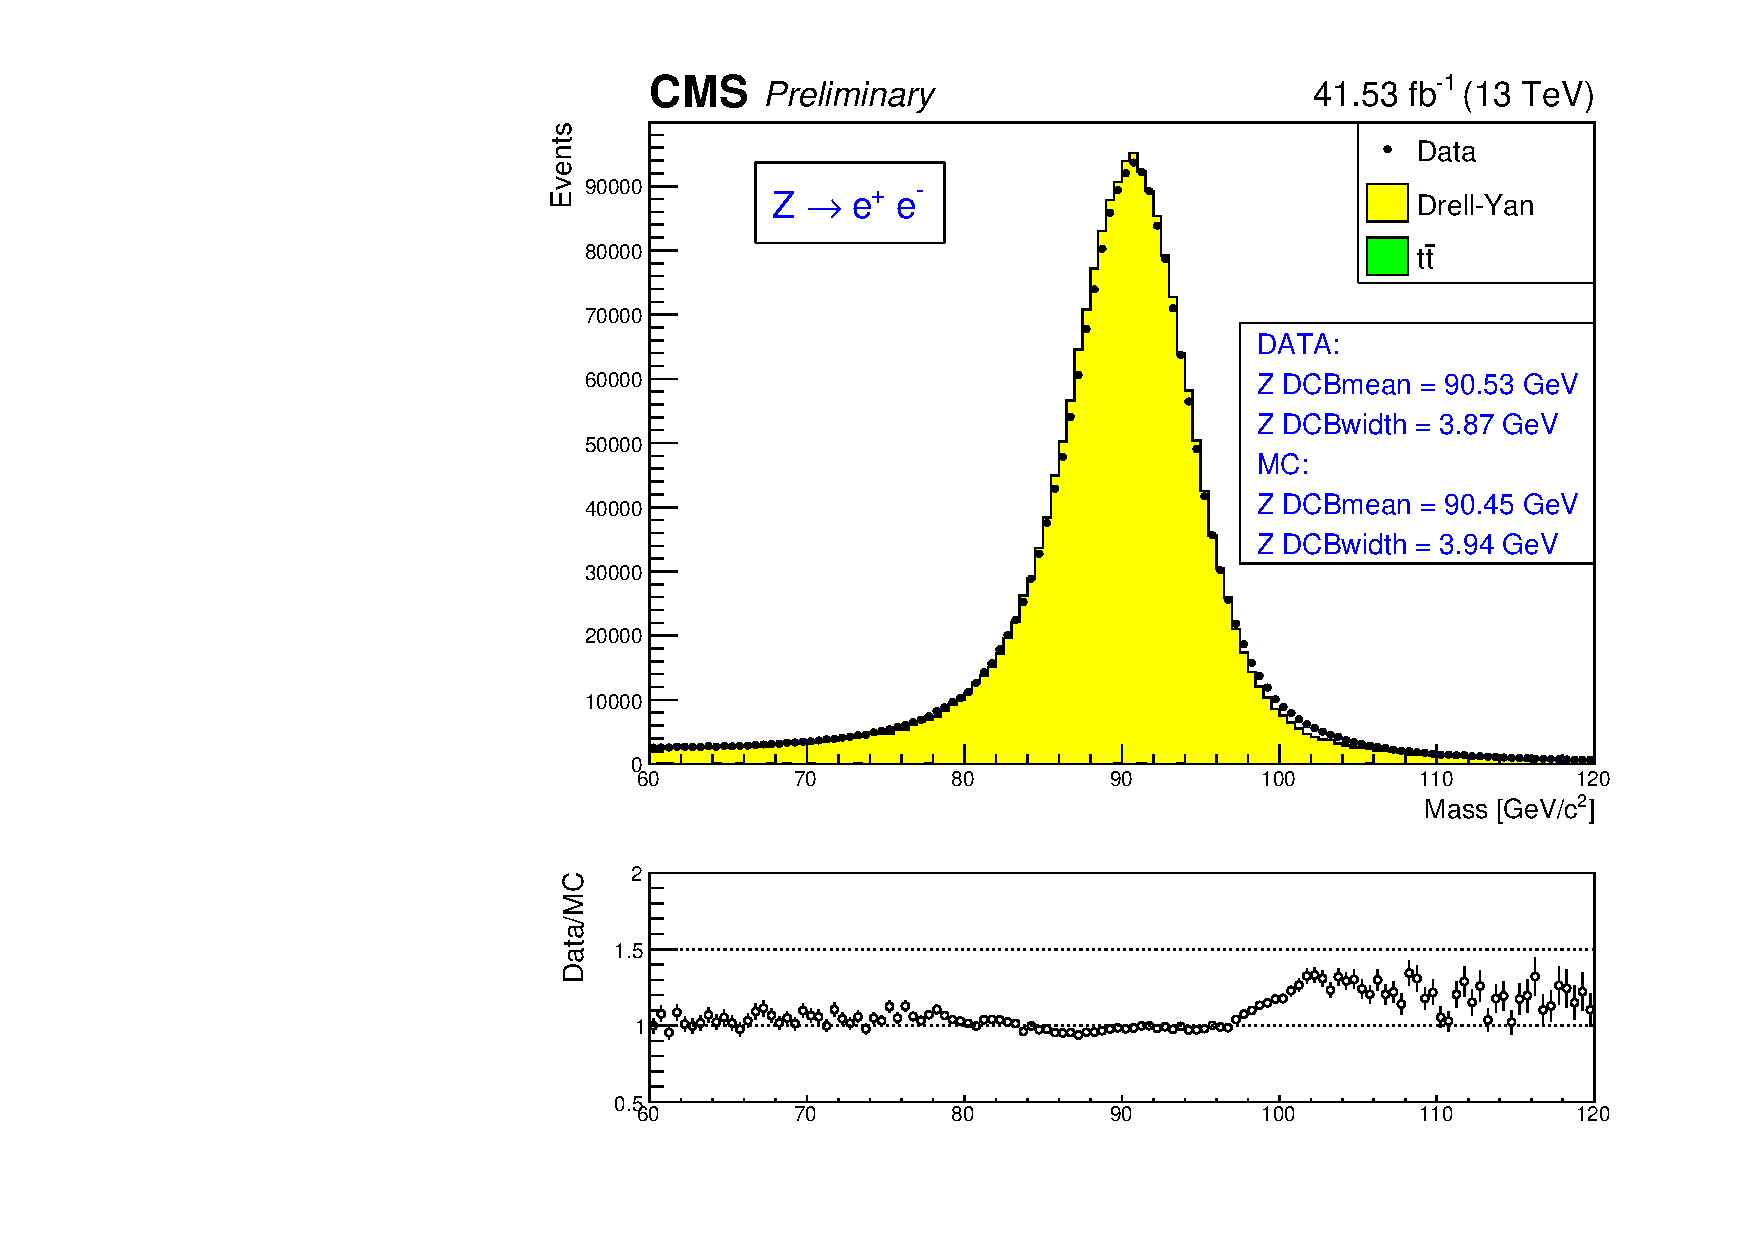
\includegraphics{Figures/Electrons/2017_ZMass_ele_EEEE.pdf}}} \\
%\end{center}
%\caption{
%(a): electron energy scale measured in the $Z\rightarrow \Pe \Pe$ control region for all electrons, for both electrons in the barrel (b), for one electron in the barrel, one in the endcaps (c) and for both electrons in the endcaps (d), for 2017 data.
%The results of the Crystall-ball fit are reported in the figures.
%%\textbf{FIXME: e-scale and smearing corrections NOT yet available and thus NOT yet applied} 
%}
%\label{fig:ele_energy_scaleB}
%\end{figure}
%
%\begin{figure}[!htb]
%\vspace*{0.3cm}
%\begin{center}
%\subfigure [] {\resizebox{8cm}{!}{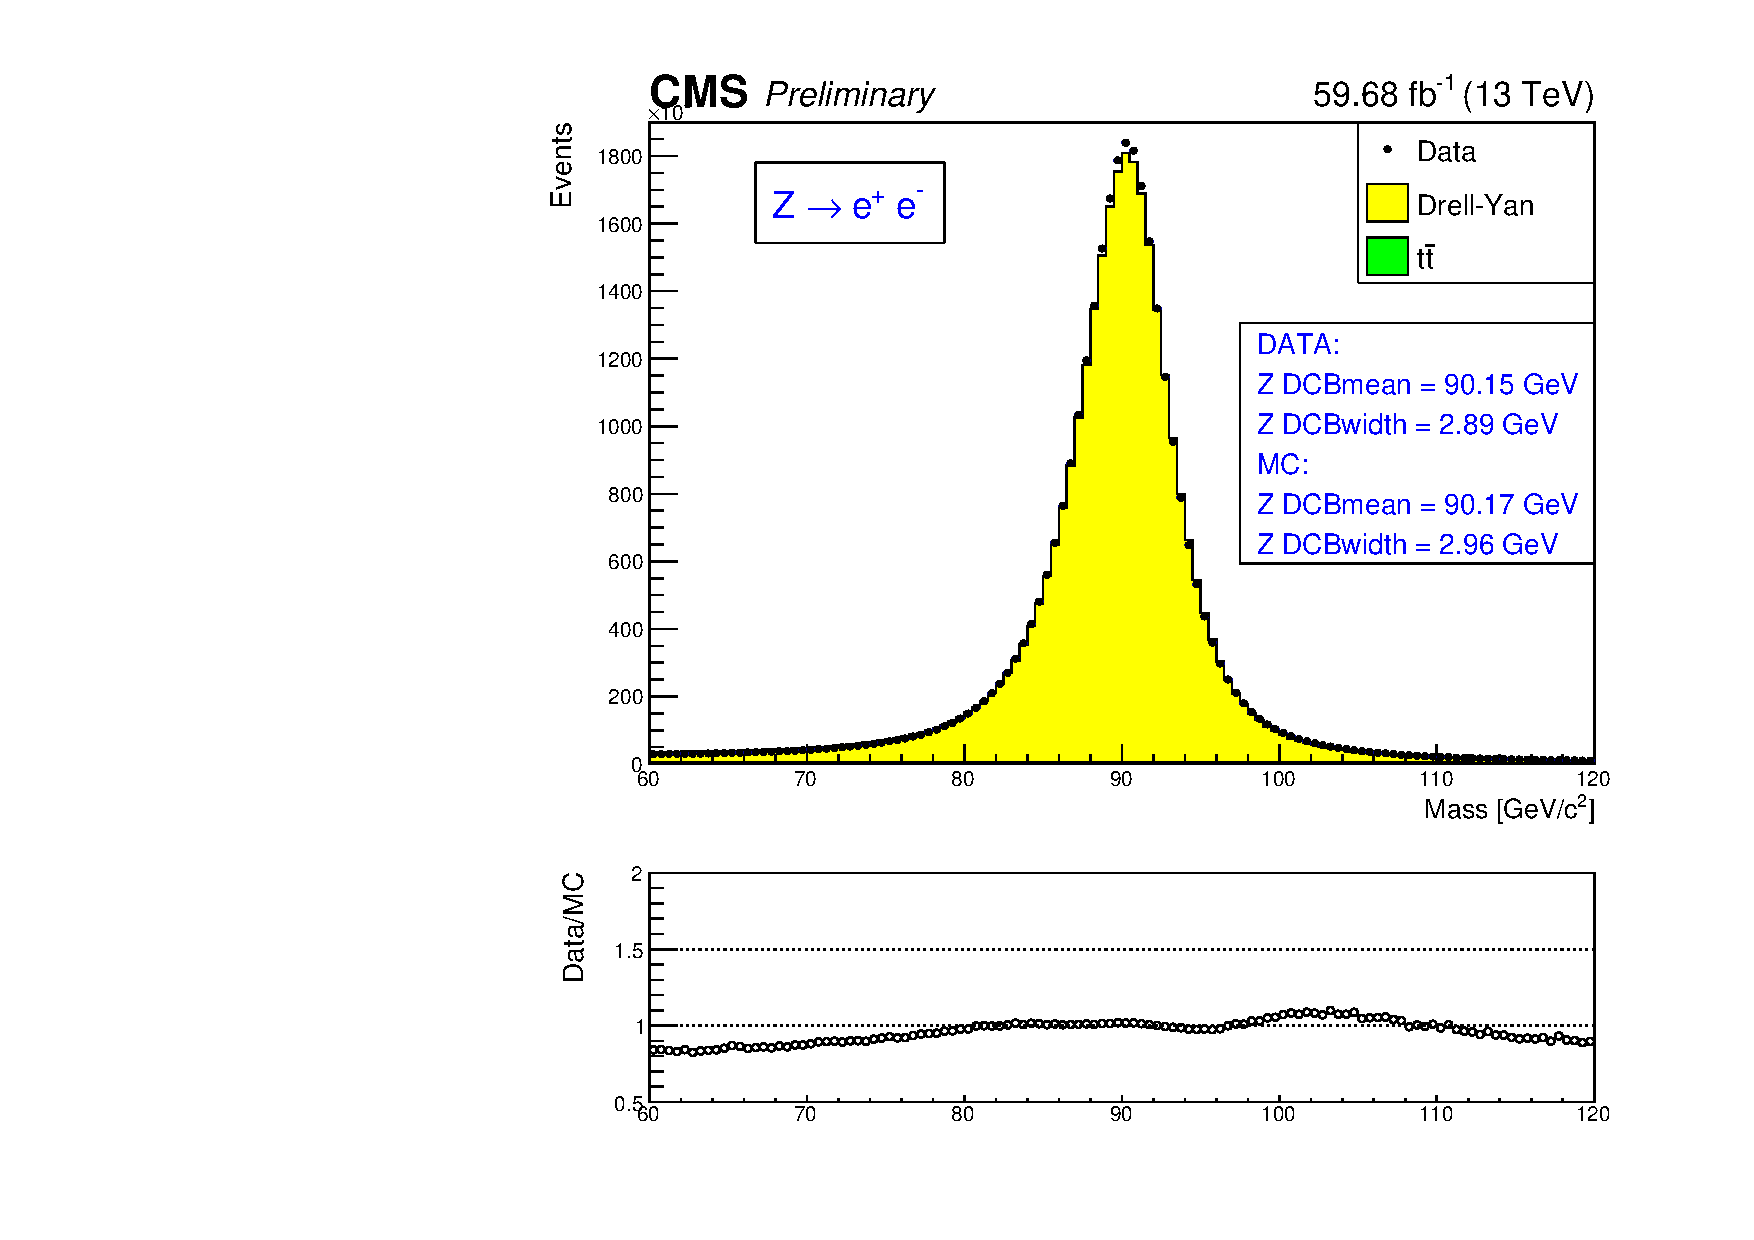
\includegraphics{Figures/Electrons/2018_ZMass_ele.pdf}}}
%\subfigure [] {\resizebox{8cm}{!}{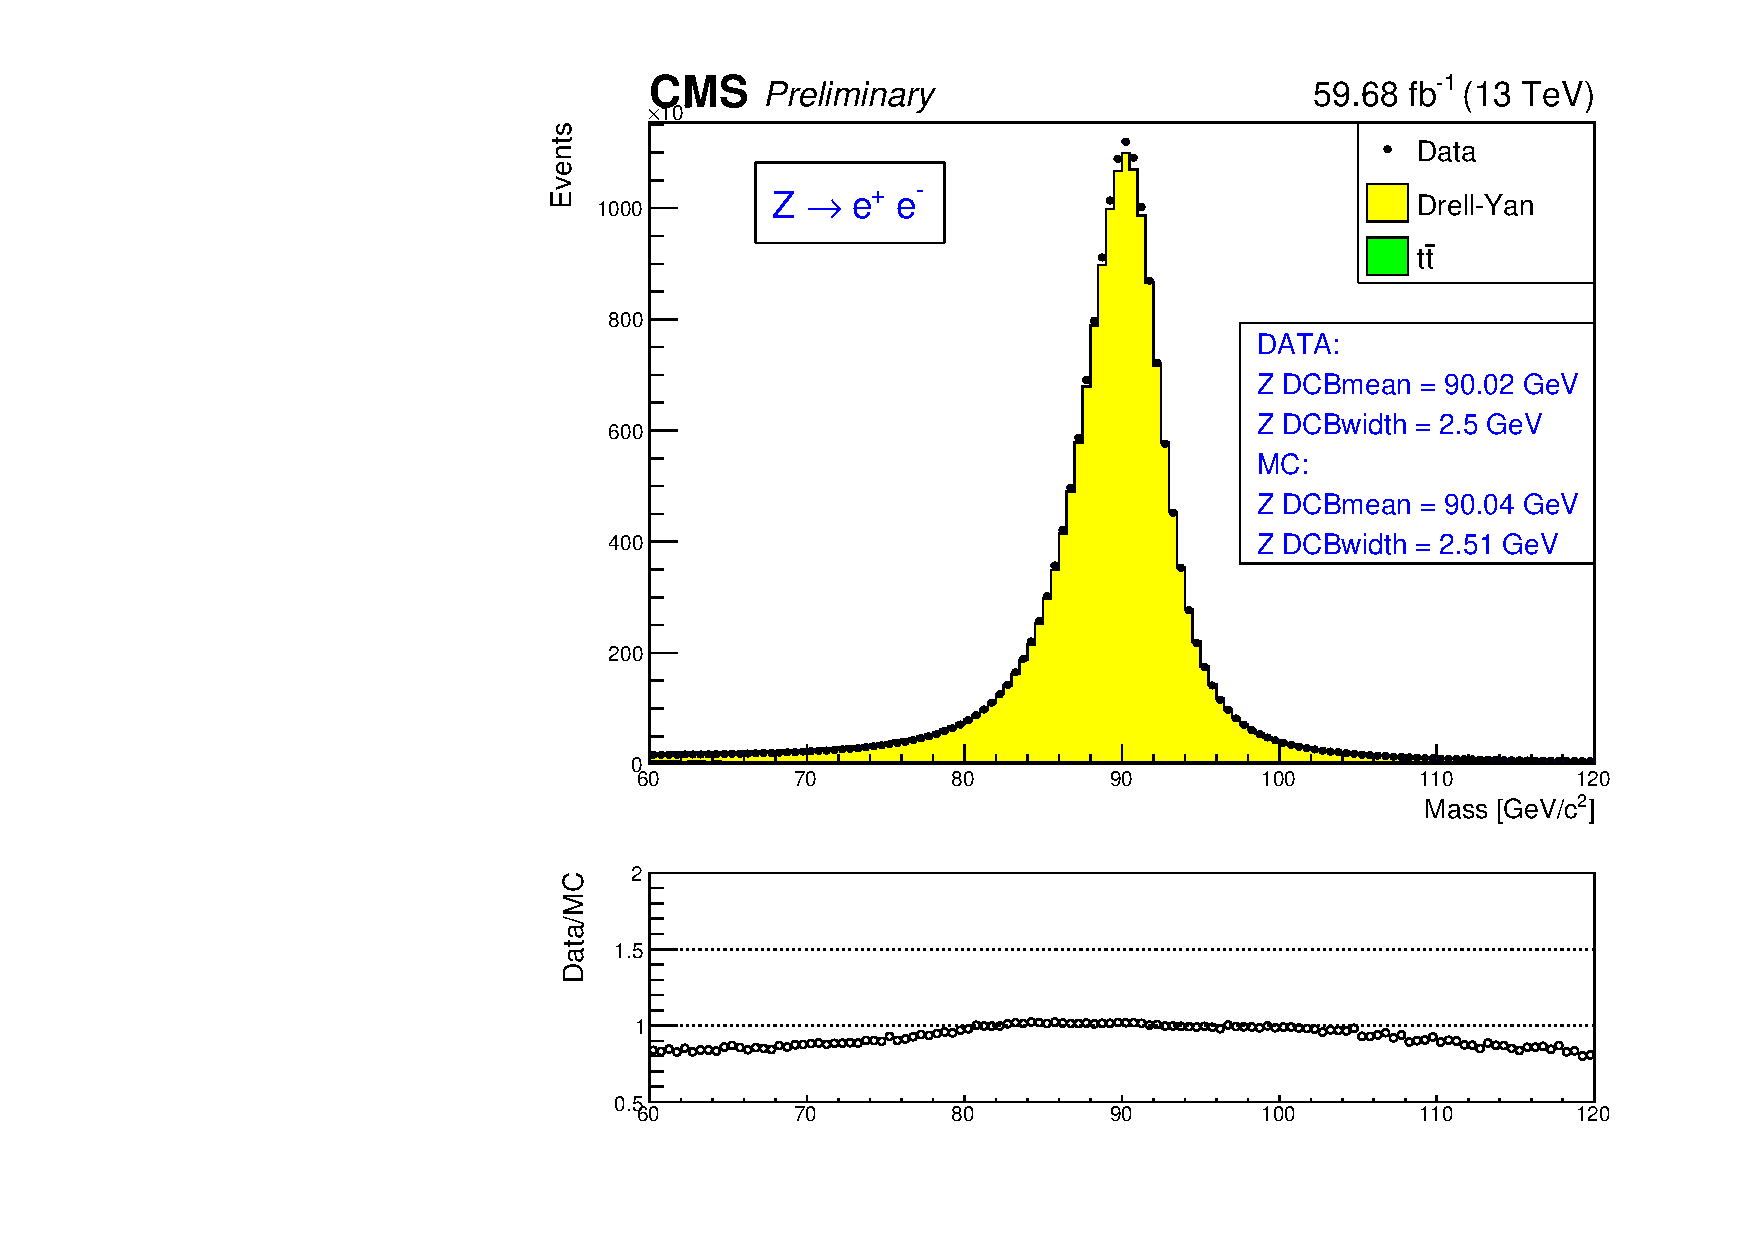
\includegraphics{Figures/Electrons/2018_ZMass_ele_EBEB.pdf}}} \\
%\subfigure [] {\resizebox{8cm}{!}{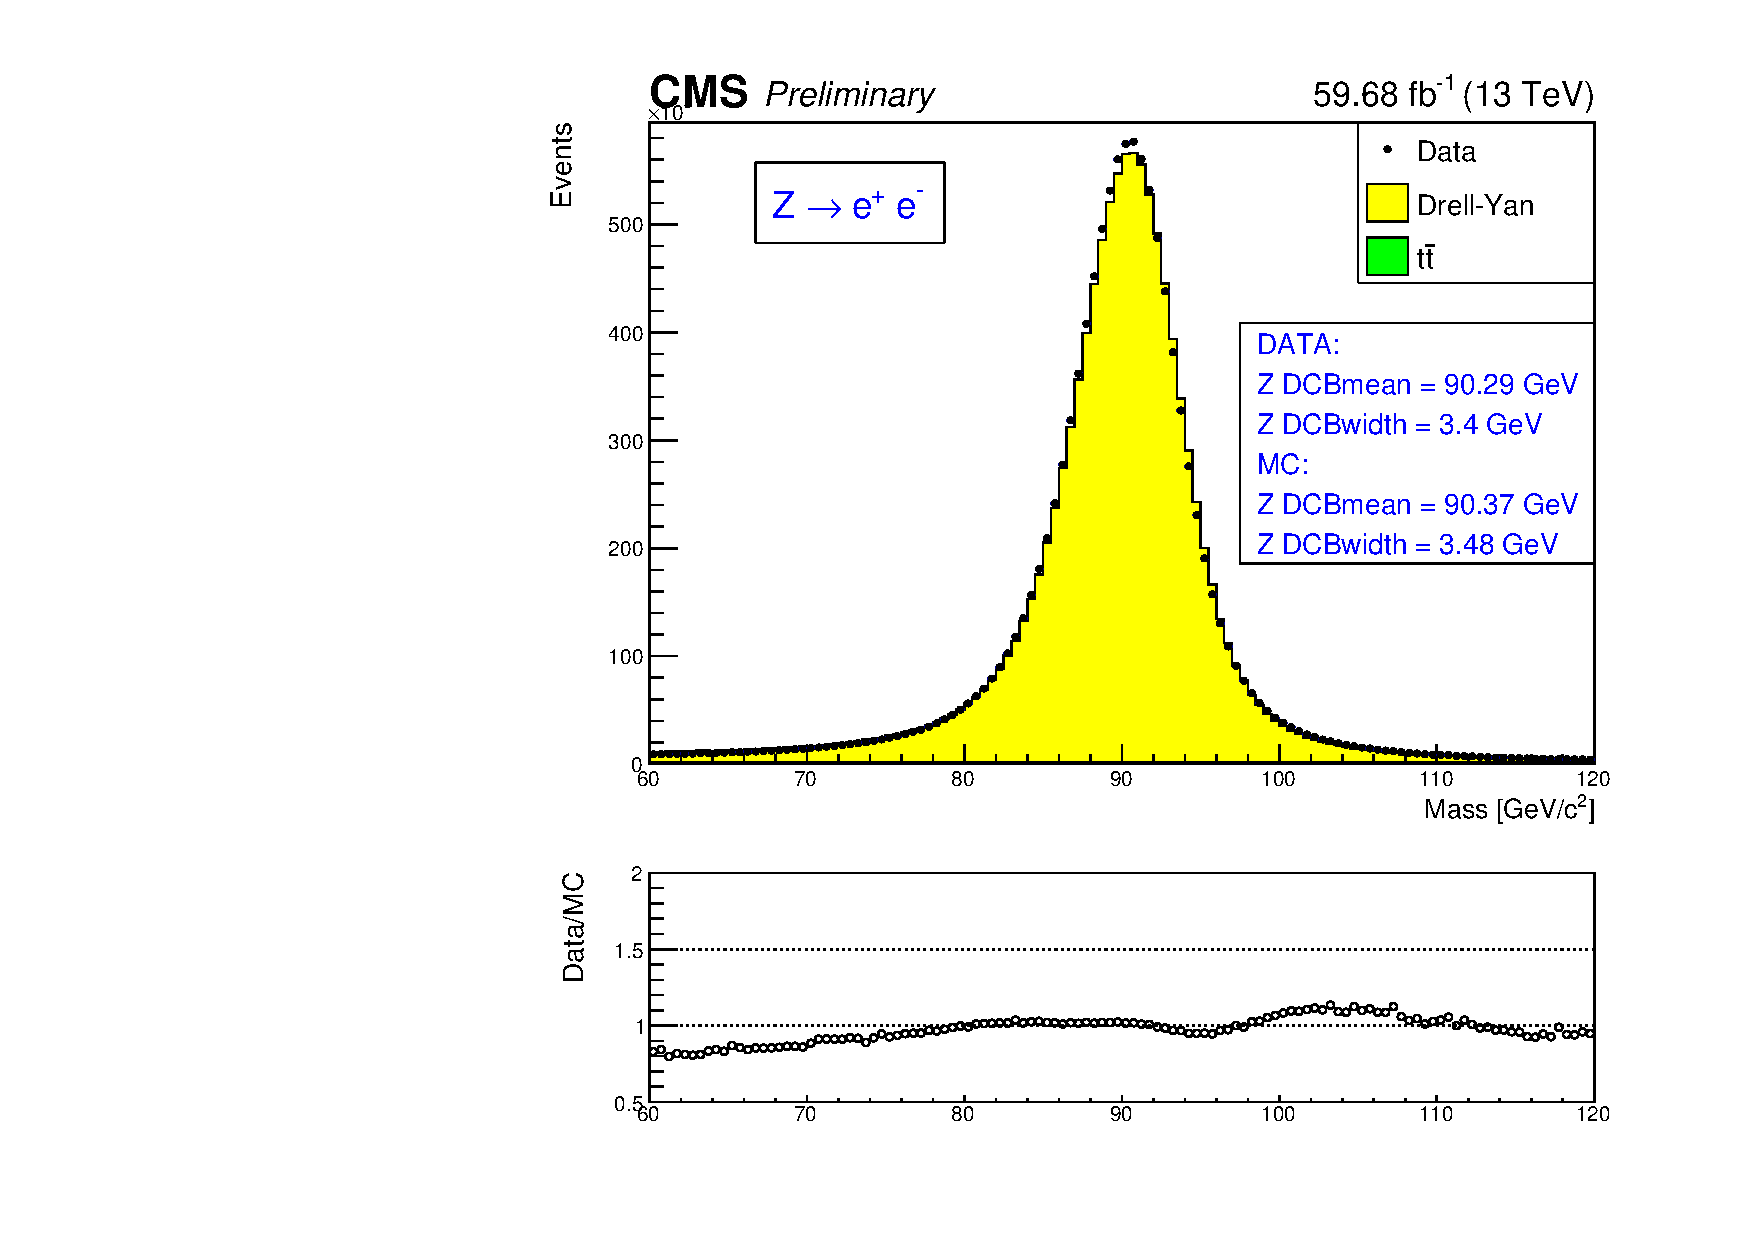
\includegraphics{Figures/Electrons/2018_ZMass_ele_EBEE.pdf}}}
%\subfigure [] {\resizebox{8cm}{!}{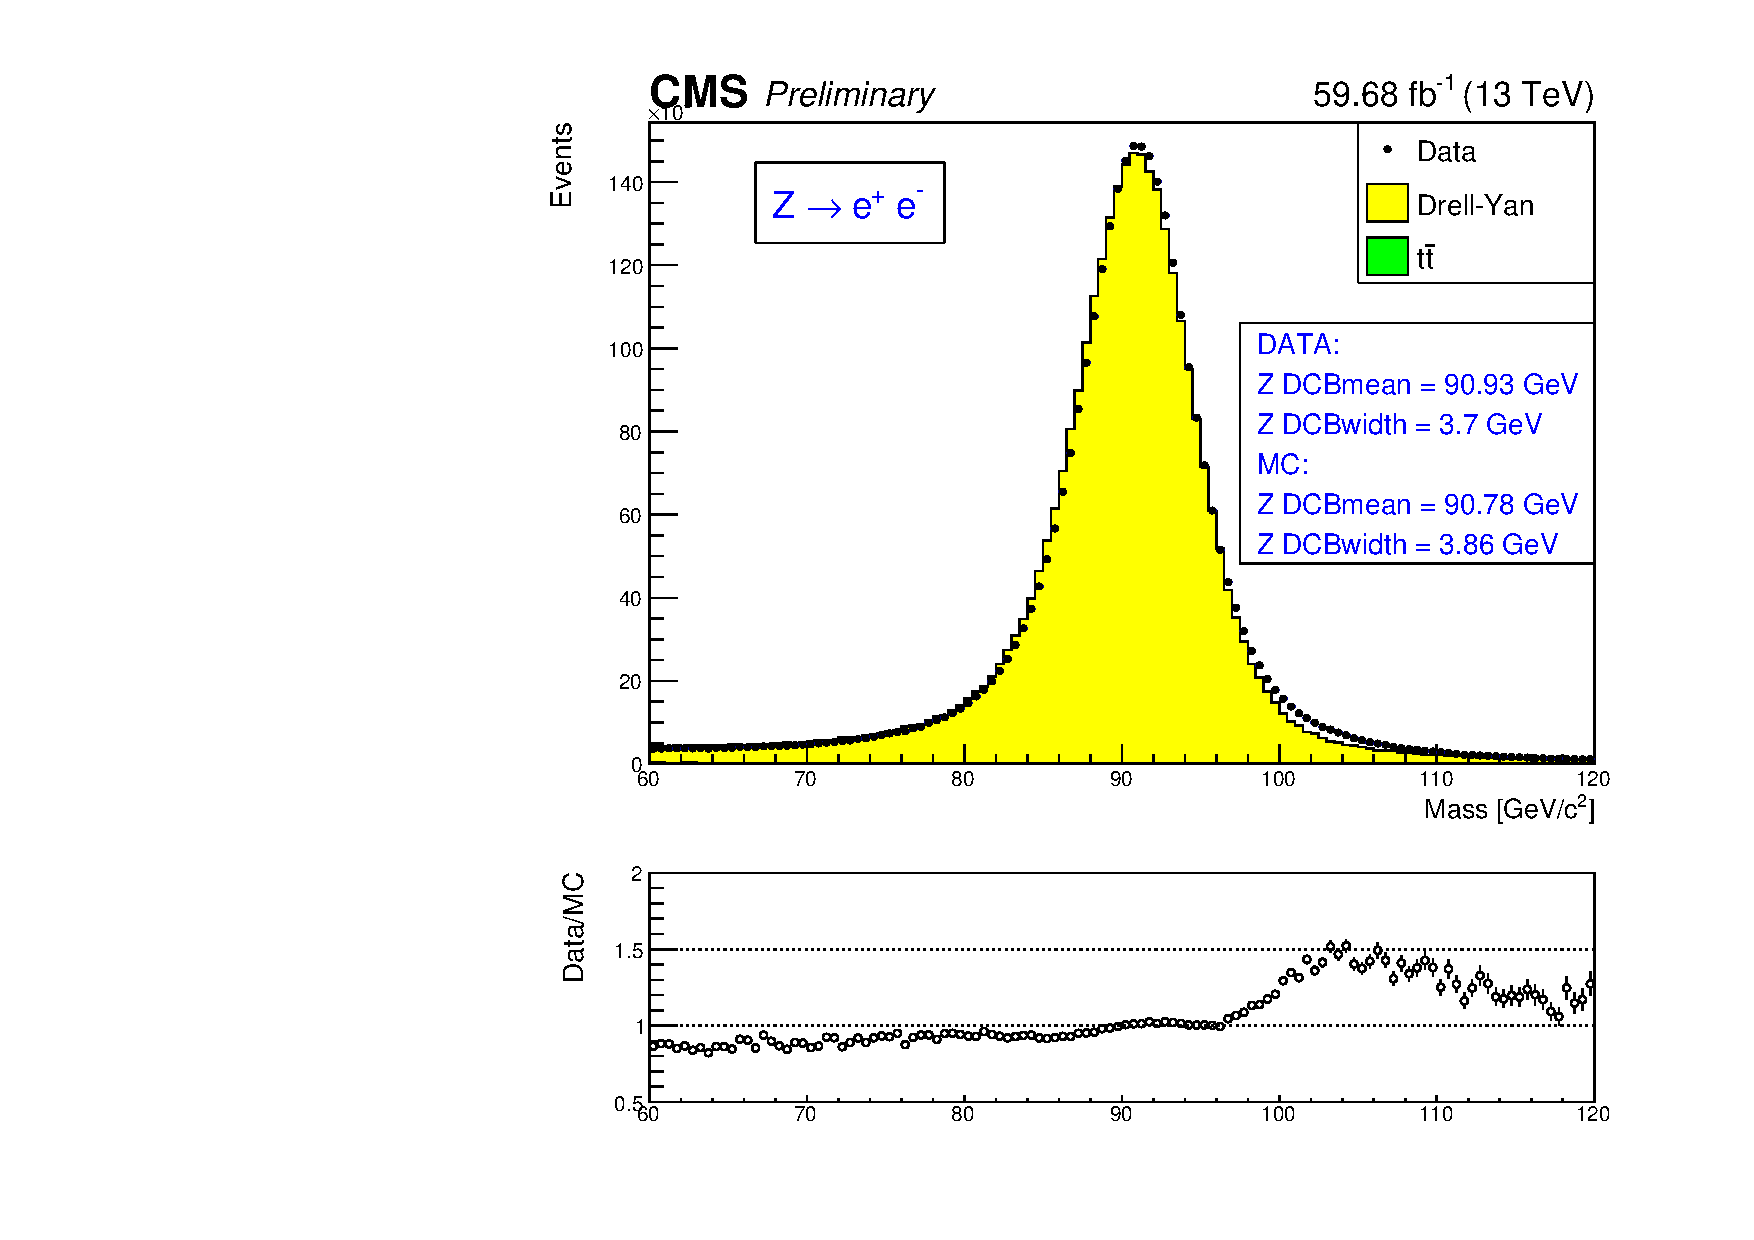
\includegraphics{Figures/Electrons/2018_ZMass_ele_EEEE.pdf}}} \\
%\end{center}
%\caption{
%(a): electron energy scale measured in the $Z\rightarrow \Pe \Pe$ control region for all electrons, for both electrons in the barrel (b), for one electron in the barrel, one in the endcaps (c) and for both electrons in the endcaps (d), for 2018 data.
%The results of the Crystall-ball fit are reported in the figures. 
%%\textbf{FIXME: e-scale and smearing corrections NOT yet available and thus NOT yet applied} 
%}
%\label{fig:ele_energy_scaleC}
%\end{figure}
%
%\clearpage

%
\subsubsection{Electron Efficiency Measurements}
\label{sec:eleEffMeas}
Referred to \cite{CMS-PAS-HIG-19-001}.

%The Tag-and-Probe study was performed on the EGM dataset using the golden JSON of ~58.83 fb$^{-1}$. More details on the Tag-and-Probe method can be found in Ref.~\cite{AN-15-277}. 
%
%Tag electrons need to satisfy the following quality requirements:
%\begin{itemize}
%%\item trigger matched to HLT\_Ele27\_eta2p1\_WPTight\_Gsf\_v*
%\item~trigger matched to single electron trigger (e.g HLT\_Ele32\_WPTight\_Gsf\_L1DoubleEG\_v* for 2018 for instance)
%\item~$p_{T} > 30$~GeV (tag), super cluster (SC) $\eta < 2.17$% but on in EB-EE gap ($1.4442<|\eta|<1.566$)
%\item~the tag and the probe need to have opposite charge.
%%\item tight working point of the Spring16 cut-based electron ID
%\end{itemize}
%
%For the bin between 7 and 20 GeV, additional criteria are required: 
%\begin{itemize}
%\item~the tag has to pass a cut on the MVA ID$>0.92$, $\sqrt(2*PFMET*p_T(tag)*(1-cos(\phi_{MET}-\phi_{tag})))<45 GeV$.
%\item~tag $p_{T}$ increased to 50 GeV
%\item~the charge is determined with the so-called selection method, asing all three estimates of the electron charge to agree.
%\end{itemize}
%%t
%These additional requirements help cleaning the background and makes the fits more reliable (and thus, the measurement more precise).
%
%Probe electrons only need to be reconstructed as GsfElectron while the FSR recovery algorithm is not applied in efficiency measurement. 
%
%The nominal MC efficiencies are evaluated from the LO MadGraph Drell-Yan, while the NLO systematics use the MadGraph\_AMCatNLO sample (or POWHEG in 2018).
%
%For the efficiency measurements a template fit is used. The $m_{ee}$ signal shape of the passing and failing probes is taken from MC and convoluted with a Gaussian. The data is then fitted with the convoluted MC template and a CMSShape (an Error-function with a one-sided exponential tail). This change follows from the usage of the T\&P tool developed by the EGM POG. For the low $p_T$ bins, a gaussian is added to the signal model for the failing probes. 
%
%%\paragraph{Electron selection efficiency measurements}\mbox{}\\
%%\label{par:Efficiency_measurements}
%
%The electron selection efficiency is measured as a function of the probe electron $p_{T}$ and its SC $\eta$, and separately for electrons falling in the ECAL gaps. Figure \ref{fig:ele_sel_pt_turn_onA},~\ref{fig:ele_sel_pt_turn_onB},~\ref{fig:ele_sel_pt_turn_onC} and~\ref{fig:ele_sel_eta_turn_onA},\ref{fig:ele_sel_eta_turn_onB},~\ref{fig:ele_sel_eta_turn_onC} show the $p_{T}$ and $\eta$ turn-on curves measured in data, for 2016, 2017 and 2018.
%% and the final 2D scale factor is shown in Fig.~\ref{fig:ele_sel_scale_factors} together with the systematic uncertainties. %These scale factors are very similar to the ICHEP figures, but more homogenous across $\eta$ and $p_{T}$ because of the higher statistics and the usage of more stable fitting routines in the new T\&P tool.
%
%%\includegraphics[page=2, width=0.4\textwidth]{Figures/Electrons/ErecoEta}\\
%
%\begin{figure}[!htb]
%\begin{center}
%    \subfigure [] {\resizebox{7.5cm}{!}{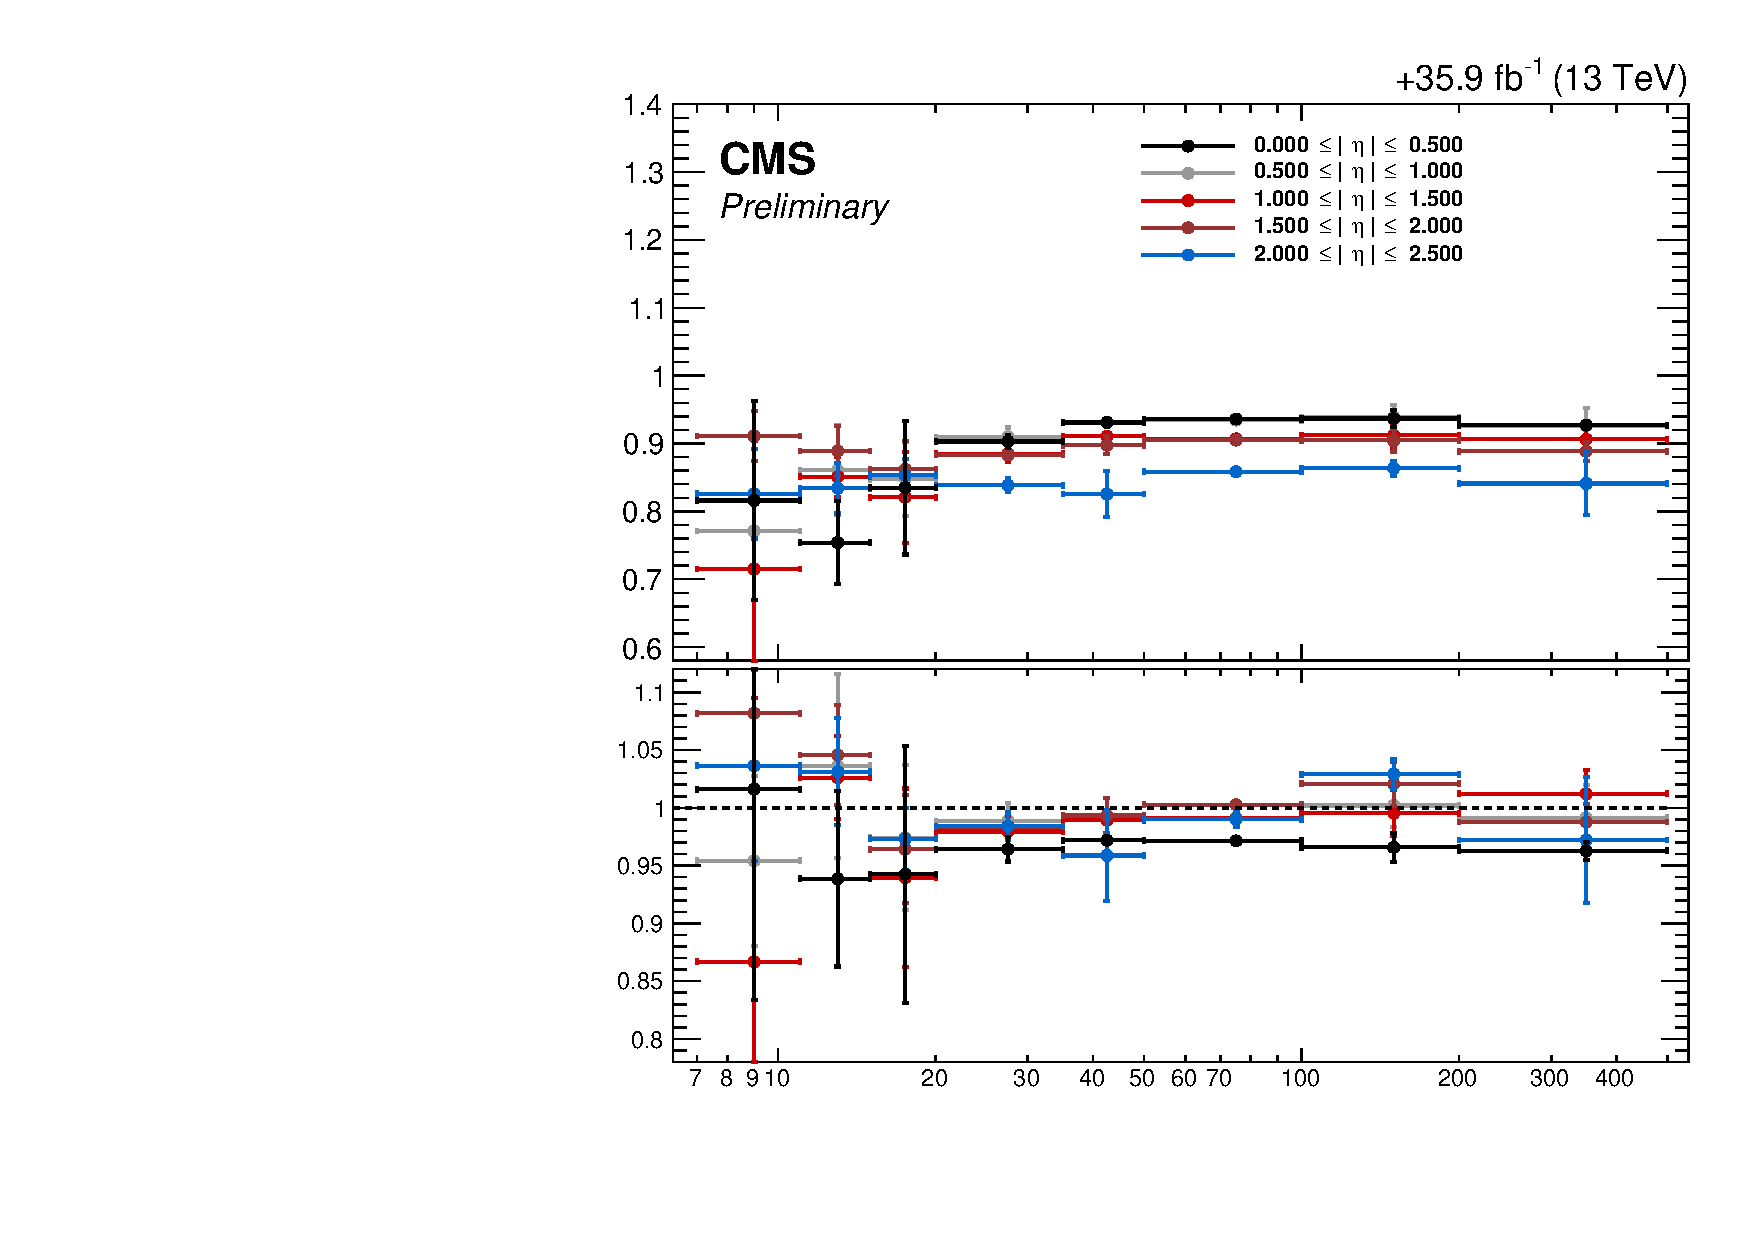
\includegraphics[page=1]{Figures/Electrons/2016_egammaEffitxt_egammaPlots.pdf}}} %eleSFvspT.png}}}
%    \subfigure [] {\resizebox{7.5cm}{!}{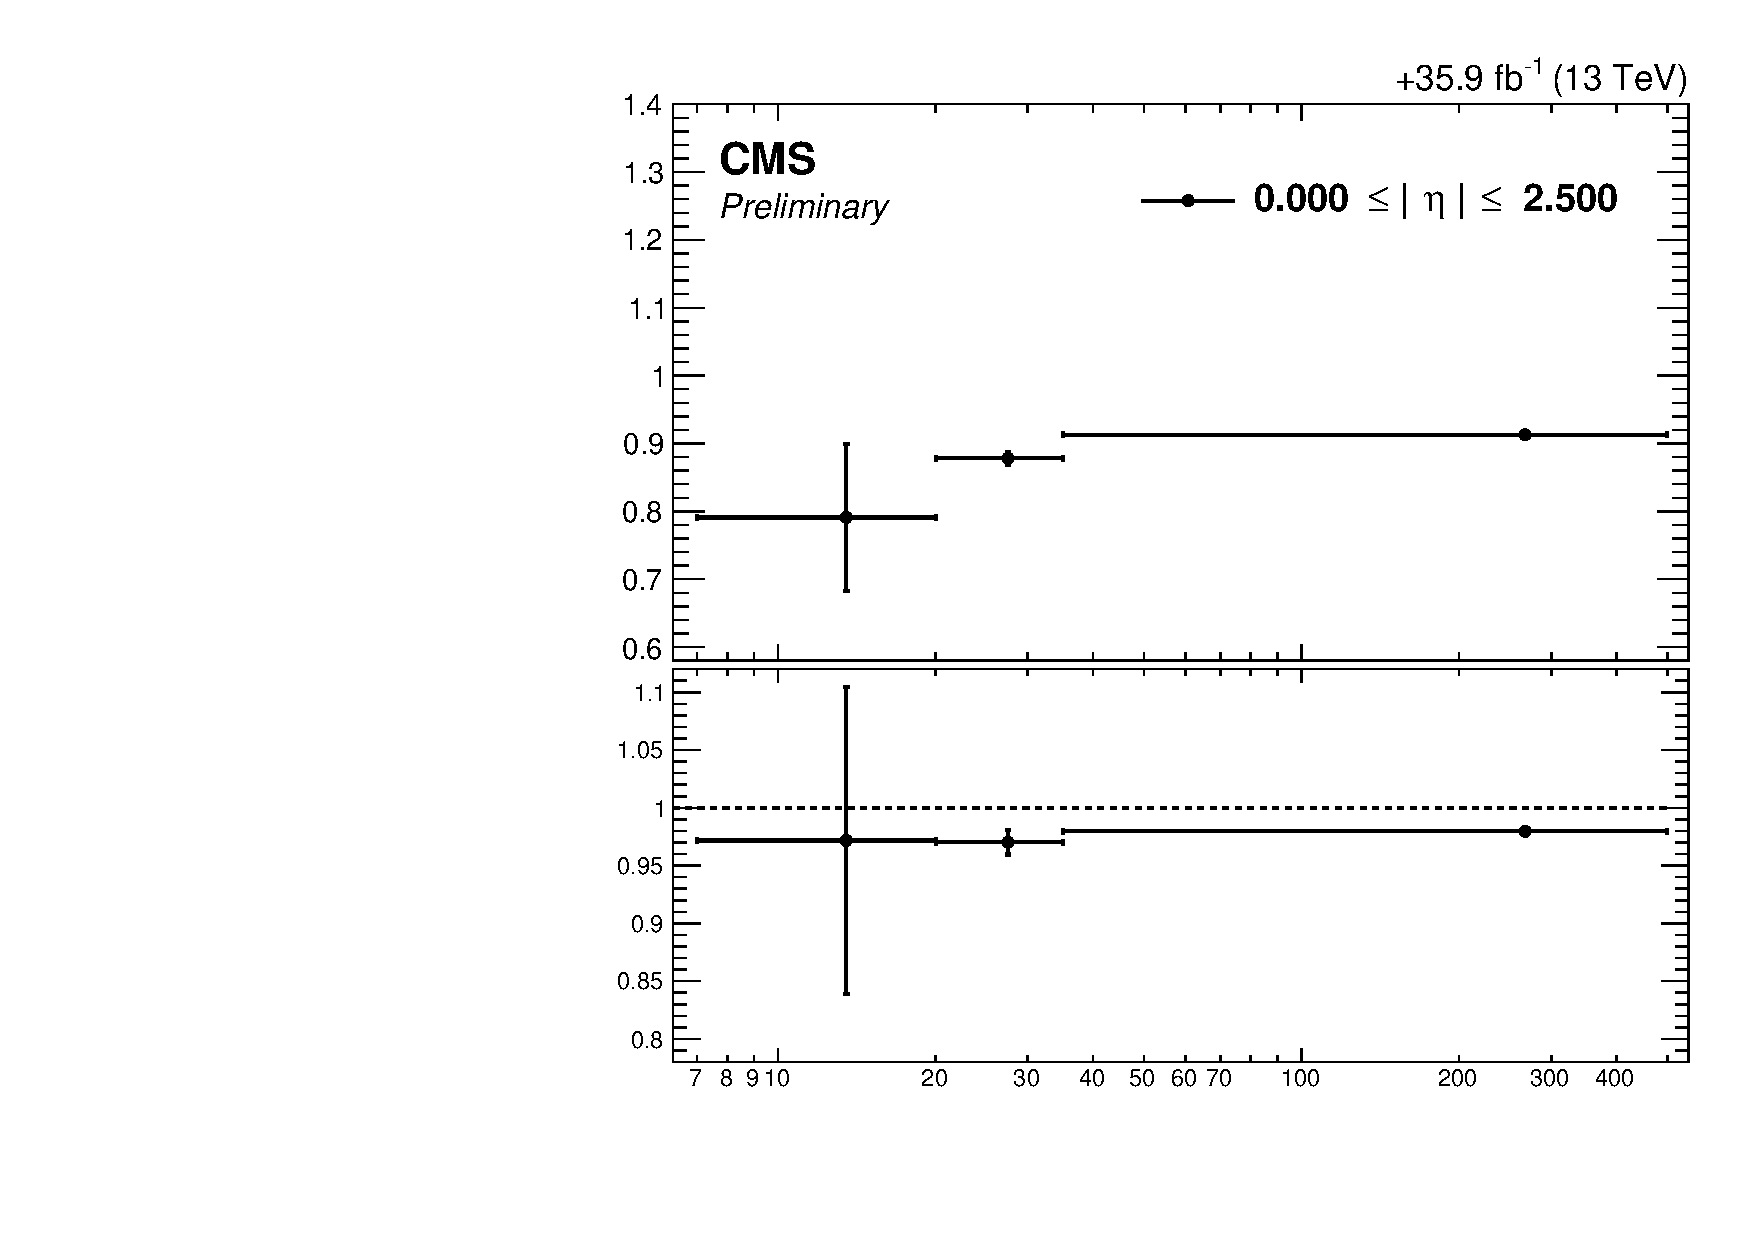
\includegraphics[page=1]{Figures/Electrons/2016_egammaEffitxt_egammaPlotsGAP.pdf}}} \\
%    %    \subfigure [] {\resizebox{7.5cm}{!}{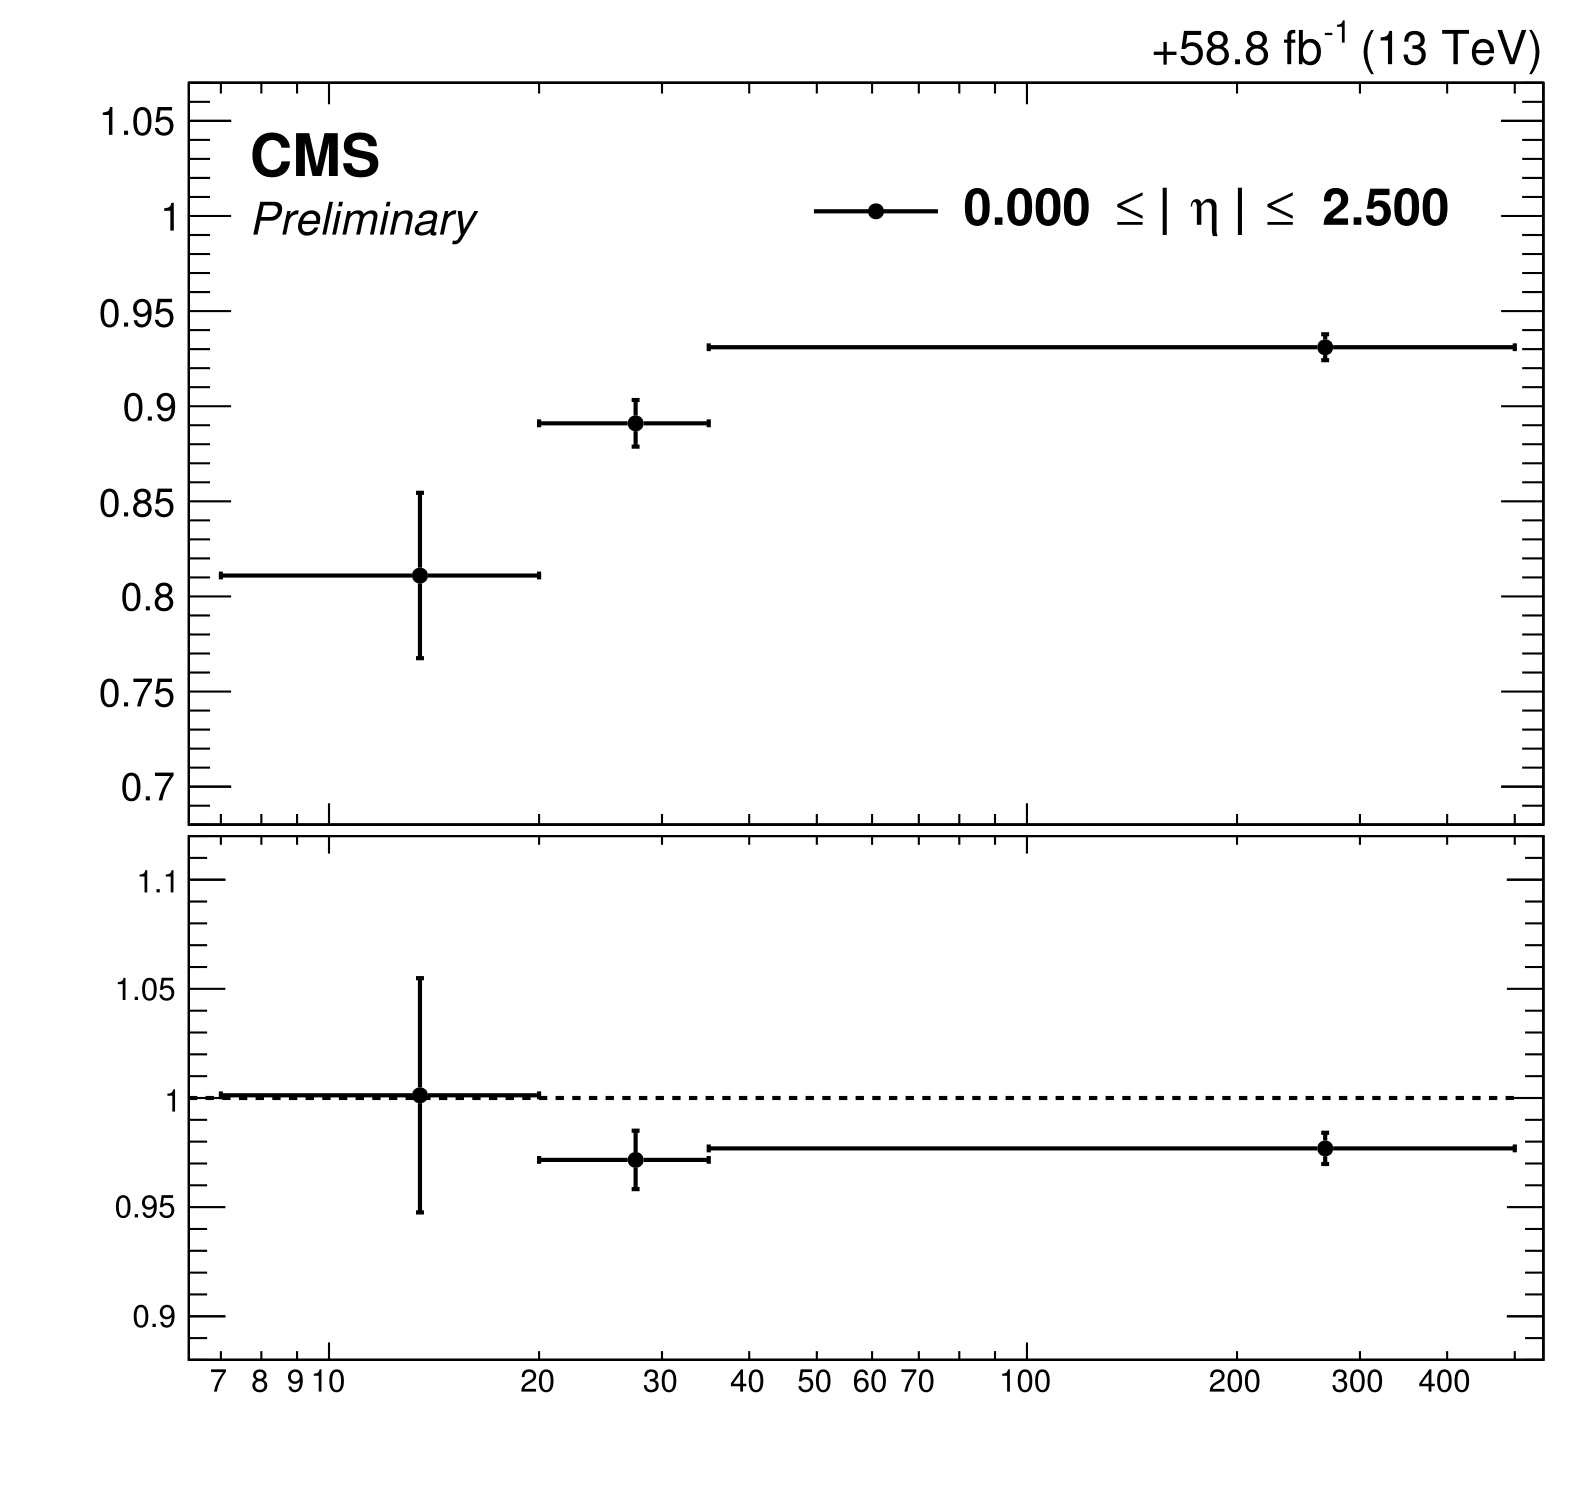
\includegraphics{Figures/Electrons/eleSFvspTgap.png}}}\\
%\caption{Electron selection efficiencies vs $p_T$ measured using the Tag-and-Probe technique described in the text, non-gap electrons (left) and gap electrons (right), together with the corresponding data/MC ratio (bottom), for 2016 samples.}
%\label{fig:ele_sel_pt_turn_onA}
%\end{center}
%\end{figure}
%
%\begin{figure}[!htb]
%\begin{center}
%    \subfigure [] {\resizebox{7.5cm}{!}{\includegraphics[page=2]{Figures/Electrons/2016_egammaEffitxt_egammaPlots.pdf}}}
%    \subfigure [] {\resizebox{7.5cm}{!}{\includegraphics[page=2]{Figures/Electrons/2016_egammaEffitxt_egammaPlotsGAP.pdf}}}\\
%\caption{Electron selection efficiencies vs $\eta$ measured using the Tag-and-Probe technique described in the text, non-gap electrons (left) and gap electrons (right), together wit the corresponding data/MC ratio at the bottom of each plot, for 2016 samples. Dashed lines is MC, solid lines is DATA.}
%\label{fig:ele_sel_eta_turn_onA}
%\end{center}
%\end{figure}
%
%\begin{figure}[!htb]
%\begin{center}
%    \subfigure [] {\resizebox{7.5cm}{!}{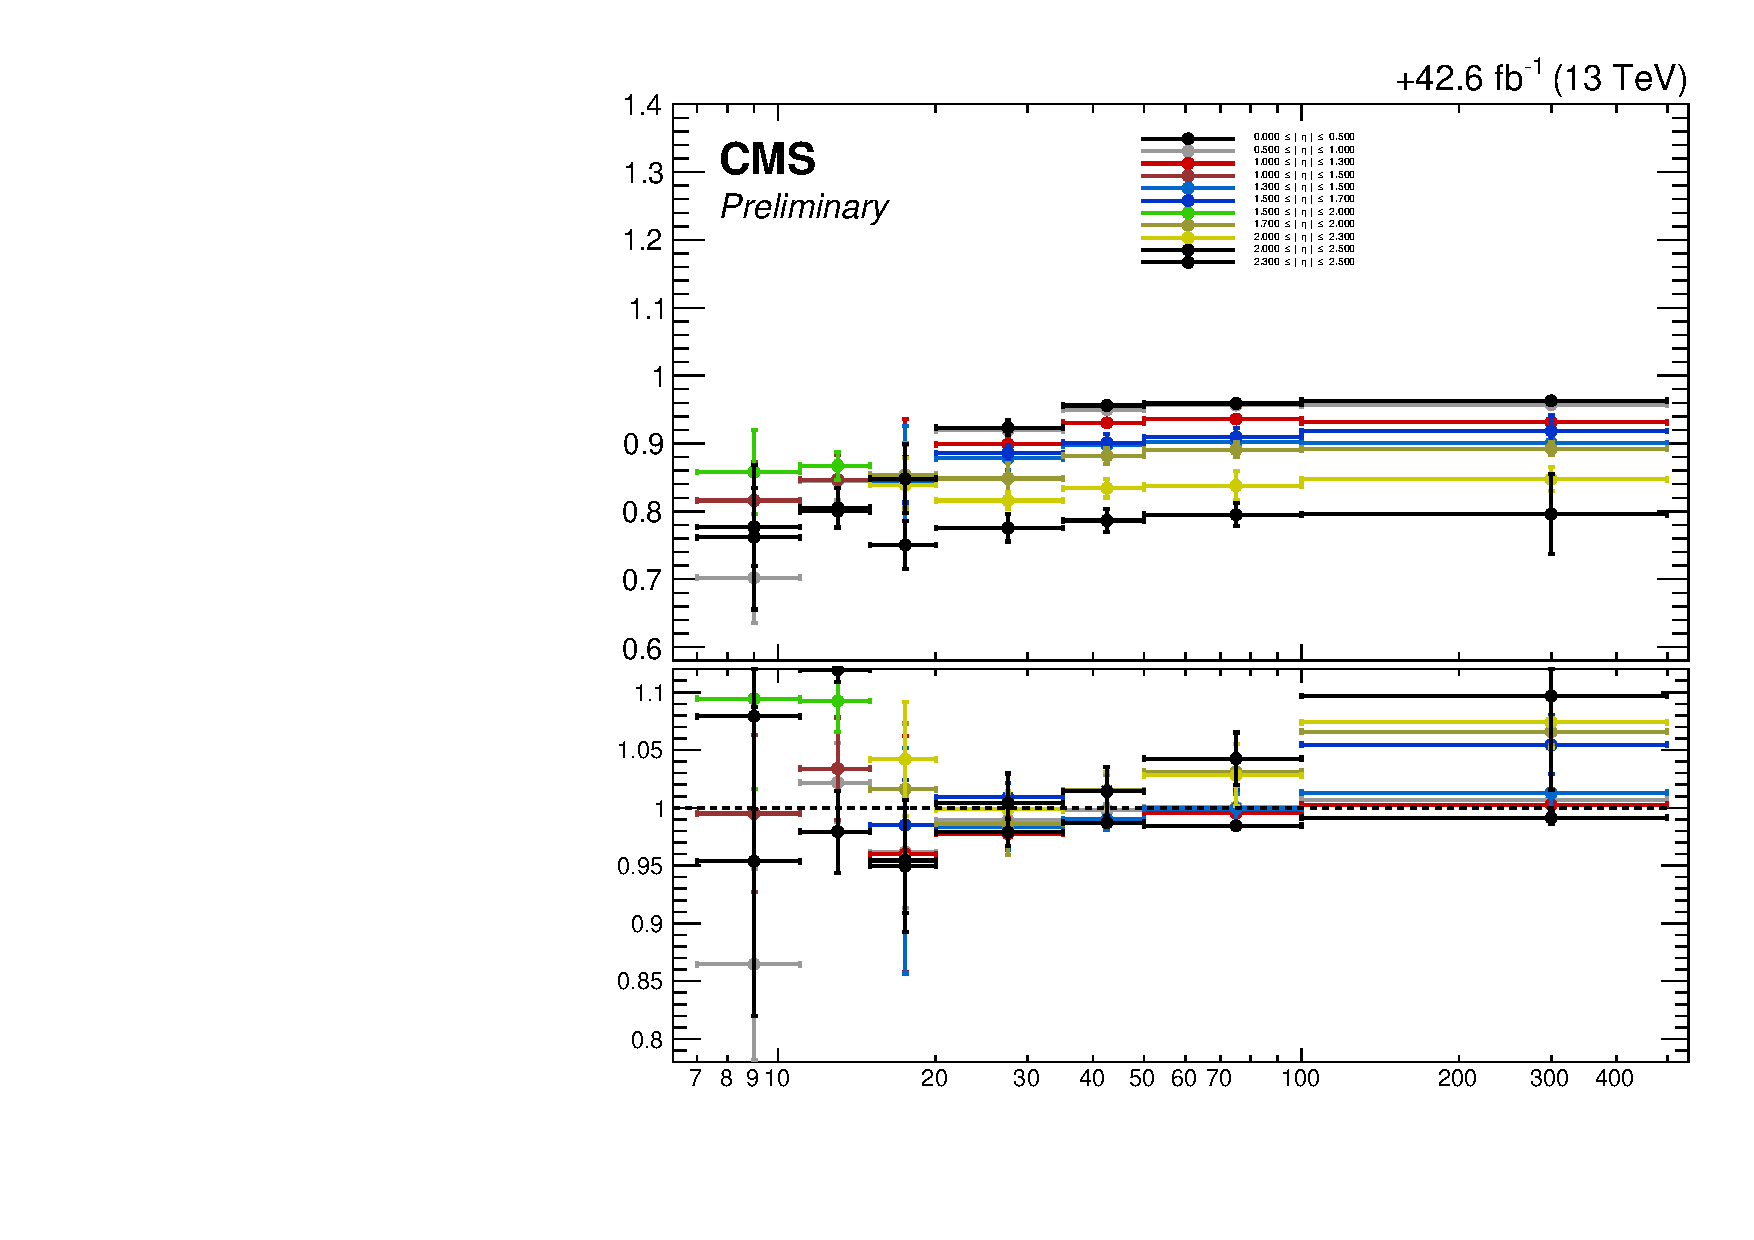
\includegraphics[page=1]{Figures/Electrons/2017_egammaEffitxt_egammaPlots.pdf}}} %eleSFvspT.png}}}
%    \subfigure [] {\resizebox{7.5cm}{!}{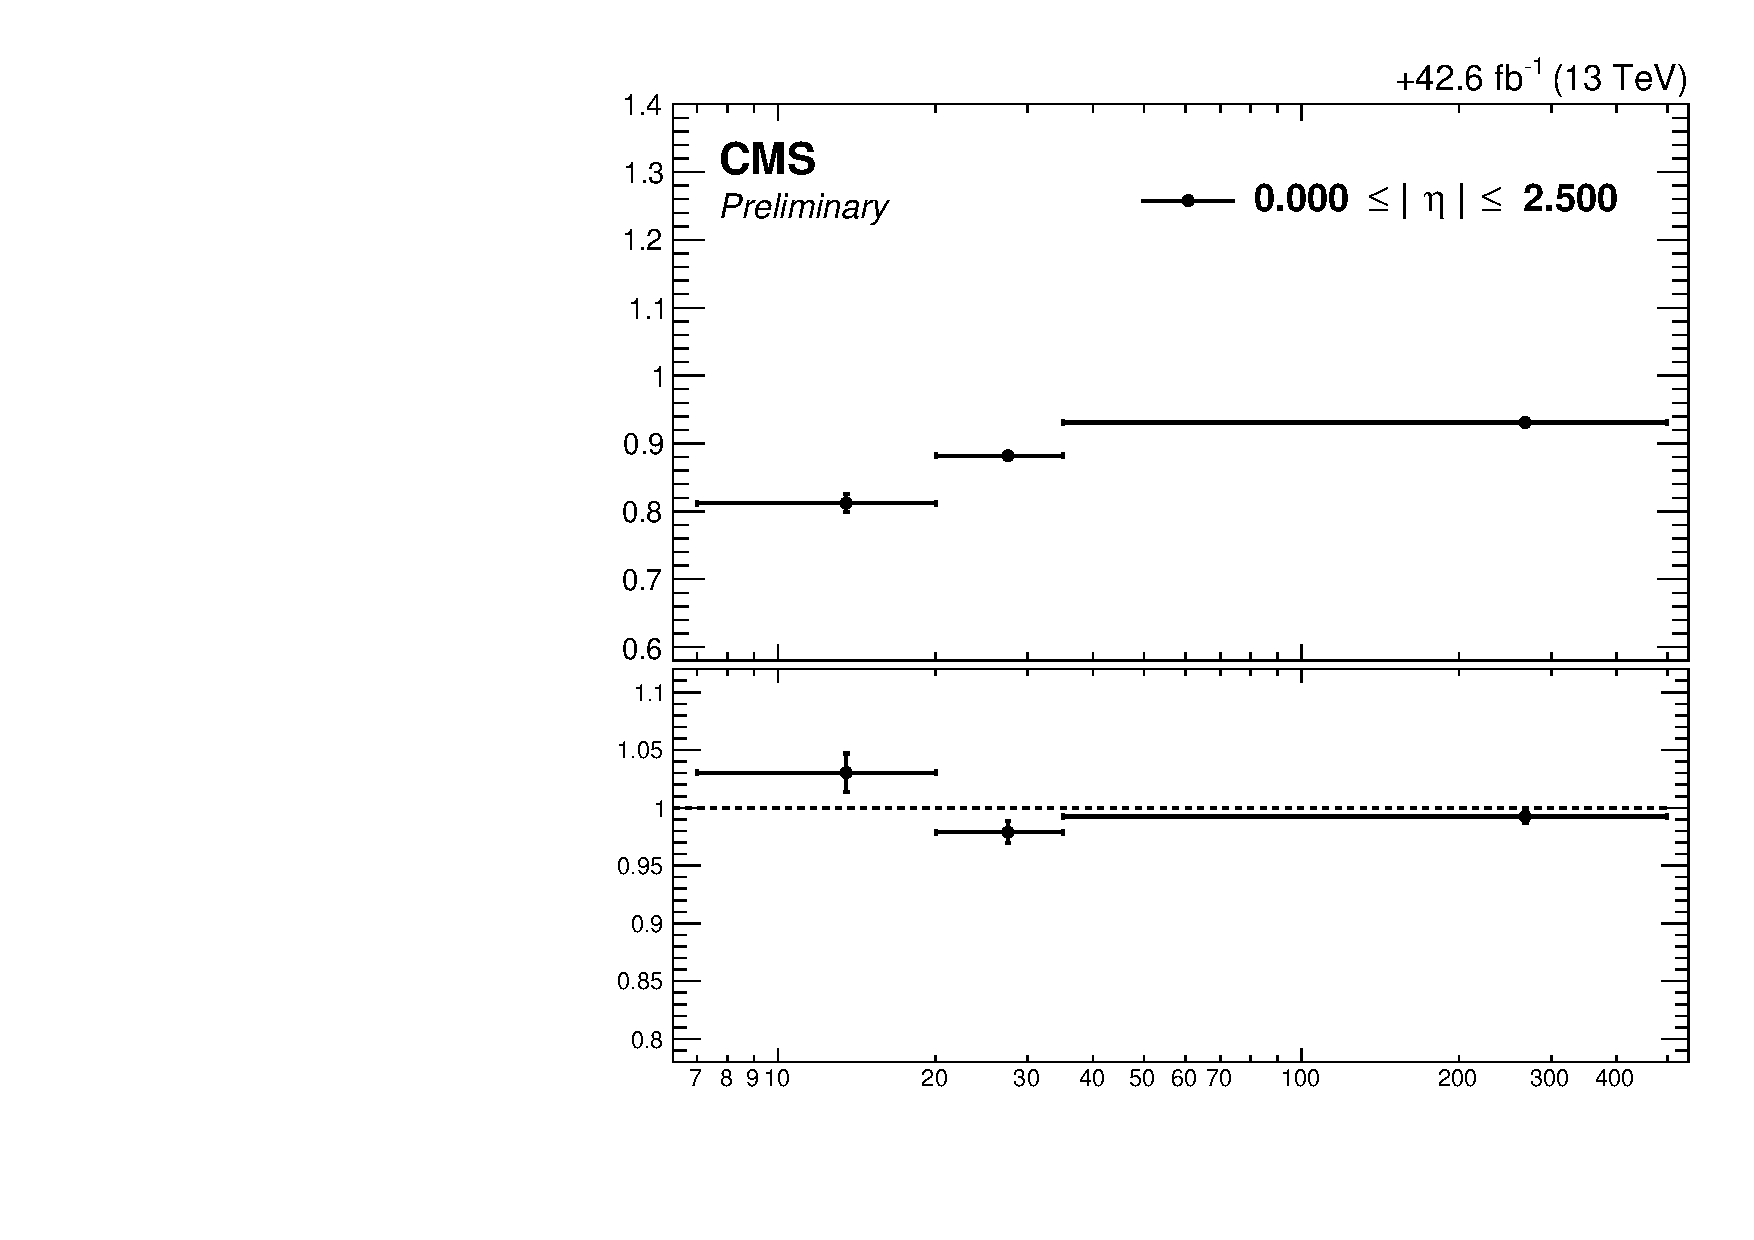
\includegraphics[page=1]{Figures/Electrons/2017_egammaEffitxt_egammaPlotsGAP.pdf}}} \\
%    %    \subfigure [] {\resizebox{7.5cm}{!}{\includegraphics{Figures/Electrons/eleSFvspTgap.png}}}\\
%\caption{Electron selection efficiencies vs $p_T$ measured using the Tag-and-Probe technique described in the text, non-gap electrons (left) and gap electrons (right), together with the corresponding data/MC ratio (bottom), for 2017 samples.}
%\label{fig:ele_sel_pt_turn_onB}
%\end{center}
%\end{figure}
%
%\begin{figure}[!htb]
%\begin{center}
%    \subfigure [] {\resizebox{7.5cm}{!}{\includegraphics[page=2]{Figures/Electrons/2017_egammaEffitxt_egammaPlots.pdf}}}
%    \subfigure [] {\resizebox{7.5cm}{!}{\includegraphics[page=2]{Figures/Electrons/2017_egammaEffitxt_egammaPlotsGAP.pdf}}}\\
%\caption{Electron selection efficiencies vs $\eta$ measured using the Tag-and-Probe technique described in the text, non-gap electrons (left) and gap electrons (right), together wit the corresponding data/MC ratio at the bottom of each plot, for 2017 samples. Dashed lines is MC, solid lines is DATA.}
%\label{fig:ele_sel_eta_turn_onB}
%\end{center}
%\end{figure}
%
%\begin{figure}[!htb]
%\begin{center}
%    \subfigure [] {\resizebox{7.5cm}{!}{\includegraphics[page=1]{Figures/Electrons/2018_egammaEffitxt_egammaPlots.pdf}}} %eleSFvspT.png}}}
%    \subfigure [] {\resizebox{7.5cm}{!}{\includegraphics[page=1]{Figures/Electrons/2018_egammaEffitxt_egammaPlotsGAP.pdf}}} \\
%    %    \subfigure [] {\resizebox{7.5cm}{!}{\includegraphics{Figures/Electrons/eleSFvspTgap.png}}}\\
%\caption{Electron selection efficiencies vs $p_T$ measured using the Tag-and-Probe technique described in the text, non-gap electrons (left) and gap electrons (right), together with the corresponding data/MC ratio (bottom), for 2018 samples.}
%\label{fig:ele_sel_pt_turn_onC}
%\end{center}
%\end{figure}
%
%\begin{figure}[!htb]
%\begin{center}
%    \subfigure [] {\resizebox{7.5cm}{!}{\includegraphics[page=2]{Figures/Electrons/2018_egammaEffitxt_egammaPlots.pdf}}}
%    \subfigure [] {\resizebox{7.5cm}{!}{\includegraphics[page=2]{Figures/Electrons/2018_egammaEffitxt_egammaPlotsGAP.pdf}}}\\
%\caption{Electron selection efficiencies vs $\eta$ measured using the Tag-and-Probe technique described in the text, non-gap electrons (left) and gap electrons (right), together wit the corresponding data/MC ratio at the bottom of each plot, for 2018 samples. Dashed lines is MC, solid lines is DATA.}
%\label{fig:ele_sel_eta_turn_onC}
%\end{center}
%\end{figure}
%
%%\begin{figure}[!htb]
%%\begin{center}
%%    \subfigure [] {\resizebox{7.5cm}{!}{\includegraphics{Figures/Placeholder.png}}}
%%    \subfigure [] {\resizebox{7.5cm}{!}{\includegraphics{Figures/Placeholder.png}}}\\
%%\caption{2D ($p_T, \eta$) Electron selection Scale Factors measured using the Tag-and-Probe technique described in the text, non-gap electrons (left) and gap electrons (right).}
%%\label{fig:ele_sel_scale_factors}
%%\end{center}
%%\end{figure}
%
%
%%\paragraph{Systematic uncertainties}\mbox{}\\
%%\label{par:Systematic_uncertainties}
%%%%%%%%%%%%%%%%%%%%%%%%%%%%%
%
% The EGM recommendations on the evaluation of Tag-and-Probe uncertainties for efficiency measurements are followed. Specifically, we consider
%
%\begin{itemize}
%   \item Variation of the signal shape from a MC shape to an analytic shape (Crystal Ball) fitted to the MC
%   \item Variation of the background shape from a CMS-shape to a simple exponential in fits to data
%%   \item Variation of the tag selection: tag $p_{T}>$35~GeV and passes MVA-based 8X ID
%   \item Using an NLO MC sample for the signal templates
%\end{itemize}
%
%The total uncertainty for the measurement of the scale factors is the quadratic sum of the statistical uncertainties returned from the fit and the aforementioned systematic uncertainties.
%
%\clearpage
%
%
%

%
%\clearpage
%
\subsection{Muons}
%
%\subsubsection{Muon Reconstruction}
\subsubsection{Muon Reconstruction and Identification}
\label{sec:muonReco}
Referred to \cite{CMS-PAS-HIG-19-001}.
%
%More details on muon reconstruction can be found in Ref.~\cite{AN-15-277}.
%We define {\bf loose muons} as the muons that satisfy  
%$p_T > 5$, $|\eta| < 2.4$, $dxy< 0.5$ cm, $dz < 1$ cm, where $dxy$ and $dz$ are 
%defined w.r.t. the PV and using the 'muonBestTrack'. Muons have to be 
%reconstructed by either the Global Muon or Tracker Muon algorithm. Standalone 
%Muon tracks that are only reconstructed in the muon system are rejected.
%Muons with \verb|muonBestTrackType==2| (standalone) are discarded even if they 
%are marked as global or tracker muons. 
%
%Loose muons with $\pt$ below 200\GeV are considered identified muons if they 
%also pass 
%%Muon BDT (see below).
%the PF muon ID (note that the naming 
%convention used for these IDs differs from the muon POG naming scheme, in which the ``tight ID'' used here is called the ``loose ID''). 
%Loose muons with $\pt$  above 200\GeV are considered identified muons if they pass the PF ID or the Tracker
%High-$\pt$ ID, the definition of which is shown in Table~\ref{tab:highPtID}.
%This relaxed definition is used to increase signal efficiency for the high-mass
%search. When a very heavy resonance decays to two $\cPZ$ bosons, both bosons
%will be very boosted. In the lab frame, the leptons coming from the decay of
%a highly boosted $\cPZ$ will be nearly collinear, and the PF ID loses 
%efficiency for muons separated by approximately $\Delta R < 0.4$, which roughly 
%corresponds to muons originating from $\cPZ$ bosons with $\pt > 500\GeV$.
%
%\begin{table}[h]
%    \begin{small}
%    \begin{center}
%    \caption{
%      The requirements for a muon to pass the Tracker High-$\pt$ ID. Note that
%      these are equivalent to the Muon POG High-$\pt$ ID with the global track 
%      requirements removed.
%      }
%    \begin{tabular}{|l|l|}
%      \hline
%      Plain-text description         & Technical description                 \\
%      \hline
%      Muon station matching          & Muon is matched to segments           \\
%                                     & in at least two muon stations         \\
%                                     & \textbf{NB: this implies the muon is} \\
%                                     & \textbf{an arbitrated tracker muon.}  \\
%      \hline                                                          
%      Good $\pt$ measurement         & $\frac{\pt}{\sigma_{\pt}} < 0.3$      \\
%      \hline
%      Vertex compatibility ($x-y$)   & $d_{xy} < 2$~mm                       \\
%      \hline
%      Vertex compatibility ($z$)     & $d_{z} < 5$~mm                        \\
%      \hline
%      Pixel hits                     & At least one pixel hit                \\
%      \hline
%      Tracker hits                   & Hits in at least six tracker layers   \\
%      \hline
%    \end{tabular}
%    \label{tab:highPtID}
%    \end{center}
%    \end{small}
%\end{table}
%
%An additional ``ghost-cleaning'' step is performed to deal with situations when a single muon
%can be incorrectly reconstructed as two or more muons:
%
%\begin{itemize}
%
%\item Tracker Muons that are not Global Muons are required to be arbitrated.
%\item If two muons are sharing 50\% or more of their segments then the muon with lower quality is removed.
%
%\end{itemize}

%
%%\subsubsection{Muon Identification, Isolation, and Impact Parameter Selection}
%%\label{sec:muon_MVA}
%%The main sources of non-prompt muons are non-isolated muons coming from decays of heavy-flavour mesons and mis-reconstructed jets usually originating from
light-flavour quarks. One of the main improvements brought in the analysis is development of new XGBoost multivariate discriminant for muon selection in all
Run 2 data taking periods.

Reconstructed muons are now fully identified by means of an e\textbf{X}treme \textbf{G}radient \textbf{Boost}ing (XGBoost) gradient boosting library already
used to identify electrons. This machine learning framework exploits observables based exclusively on tracking, information from the muon part of the detector
as well as different components of the isolation. The full list of used features can be found in the Table~\ref{tab:muon_MVA_input_variables}.

\begin{table}[H]
\scriptsize
   \centering
   \begin{tabular}{c|l}
\hline
\hline
Observable type & Observable name \\
\hline
\multirow{1}{*}{Kinematic variables}
	& Pseudorapidity $\eta$ \\
\hline
\multirow{2}{*}{Global track quality variables}
	& Global number of valid muon hits\\
	& Normalized Chi2 \\
\hline
\multirow{5}{*}{Track quality variables}
   & Number of valid hits \\
   & Number of valid pixel hits \\
   & SIP3D \\
   & $d_z$ \\
   & $d_{xy}$ \\
\hline
\multirow{3}{*}{Isolation variables}
   & Particle Flow photon isolation sum \\
   & Particle Flow charged hadrons isolation sum \\
   & Particle Flow neutral hadrons isolation sum \\
\hline
\multirow{1}{*}{For PU-resilience}
   & Mean energy density in the event: $\rho$ $(\mathord{\cdot})$ \\
\hline
\hline
     \end{tabular}
\small
    \caption{Overview of input features passed to the identification classifier.}
    \label{tab:muon_MVA_input_variables}
\end{table}

The muons are preselected by requiring $p_T > 5$, $|\eta| < 2.4$, $dxy< 0.5$ cm, $dz < 1$ cm, where $dxy$ and $dz$. Additionally, muons have to be reconstructed
by either the Global Muon or Tracker Muon algorithm. The signal consists of prompt muons matched to truth muons while background is composed of unmatched and true
but non-prompt muons. The MVA models are trained on 2016, 2017, and 2018 Drell-Yan with jets MC sample for both signal and background. The dedicated training for
each of the Run 2 three data taking periods guarantees optimal performance. The simulated samples used to train the model are listed bellow.

\begin{itemize}
\item \textbf{2016} \begin{verbatim}/DYJetsToLL_M-50_TuneCUETP8M1_13TeV-amcatnloFXFX-pythia8/RunIISummer16MiniAODv2-PUMoriond17_80X_mcRun2_asymptotic_2016_TrancheIV_v6_ext2-v1/MINIAODSIM\end{verbatim}
\item \textbf{2017} \begin{verbatim}/DYJetsToLL_M-50_TuneCP5_13TeV-amcatnloFXFX-pythia8/RunIIFall17MiniAOD-94X_mc2017_realistic_v10-v1/MINIAODSIM\end{verbatim}
\item \textbf{2018} \begin{verbatim}/DYJetsToLL_M-50_TuneCP5_13TeV-amcatnloFXFX-pythia8/RunIISpring18MiniAOD-100X_upgrade2018_realistic_v10-v1/MINIAODSIM\end{verbatim}
\end{itemize}

Some distributions of variables used in the training are shown in Fig.~\ref{fig:mu_features_2016}.

\begin{figure}[!htb]
   \vspace*{0.3cm}
   \begin{center}
      \includegraphics[width=0.45\textwidth]{Figures/Muons/mu_eta_5.pdf}
      \includegraphics[width=0.45\textwidth]{Figures/Muons/mu_eta_10.pdf} \\
      \includegraphics[width=0.45\textwidth]{Figures/Muons/mu_chi_square_5.pdf}
      \includegraphics[width=0.45\textwidth]{Figures/Muons/mu_chi_square_10.pdf} \\
      \includegraphics[width=0.45\textwidth]{Figures/Muons/mu_pf_photon_iso_5.pdf}
      \includegraphics[width=0.45\textwidth]{Figures/Muons/mu_pf_photon_iso_10.pdf} \\
      \includegraphics[width=0.45\textwidth]{Figures/Muons/mu_N_pixel_hits_5.pdf}
      \includegraphics[width=0.45\textwidth]{Figures/Muons/mu_N_pixel_hits_10.pdf} \\
   \caption{Distributions of some features used as the input for the MVA training on 2016 Drell-Yan with jets MC sample. Distributions are shown for muons with
   $5 < p_T < 10 $ GeV (left) and $p_T > 10$ GeV (right).}
   \label{fig:mu_features_2016}}
   \end{center}
\end{figure}

The working point (WP) is choosen as follows: yields of 3 main processes in the signal region are calculated using different WPs for different Muon MVA signal
efficiencies:

\begin{itemize}
   \item Low $p_T$ scanned in steps of 5\% (75\% - 95\%), high $p_T$ in steps of 1\% (95\% - 99\%).
   \item Our previous PF muon ID + RelPFiso + SIP3D efficiency was 75\% - 95\%.
   \item Z+X estimated using SS method only with recalculated Fake Rates for each WP.
   \item Plot $S/\sqrt(S+B)$ in search for the optimal WP choice.
\end{itemize}

The MVA score distribution together with the Working Point choice is shown in the Fig.~\ref{fig:mu_MVA_score_2016} for 2016, Fig.~\ref{fig:mu_MVA_score_2017}
for 2017, and Fig.~\ref{fig:mu_MVA_score_2018} for 2018 data taking periods.

\begin{figure}[!htb]
   \vspace*{0.3cm}
   \begin{center}
      \includegraphics[width=0.95\textwidth]{Figures/Muons/MVA_score_5_2016.pdf}\\
      \includegraphics[width=0.95\textwidth]{Figures/Muons/MVA_score_10_2016.pdf}
   \caption{The MVA score and Working Point choice for the MVA trained on 2016 Drell-Yan with jets MC sample. The MVA score is shown for muons with
   $5 < p_T < 10 $ GeV (top) and $p_T > 10$ GeV (bottom).}
   \label{fig:mu_MVA_score_2017}
   \end{center}
\end{figure}

\begin{figure}[!htb]
   \vspace*{0.3cm}
   \begin{center}
      \includegraphics[width=0.95\textwidth]{Figures/Muons/MVA_score_5_2017.pdf}\\
      \includegraphics[width=0.95\textwidth]{Figures/Muons/MVA_score_10_2017.pdf}
   \caption{The MVA score and Working Point choice for the MVA trained on 2017 Drell-Yan with jets MC sample. The MVA score is shown for muons with
   $5 < p_T < 10 $ GeV (top) and $p_T > 10$ GeV (bottom).}
   \label{fig:mu_MVA_score_2017}
   \end{center}
\end{figure}

\begin{figure}[!htb]
   \vspace*{0.3cm}
   \begin{center}
      \includegraphics[width=0.95\textwidth]{Figures/Muons/MVA_score_5_2018.pdf}\\
      \includegraphics[width=0.95\textwidth]{Figures/Muons/MVA_score_10_2018.pdf}
   \caption{The MVA score and Working Point choice for the MVA trained on 2018 Drell-Yan with jets MC sample. The MVA score is shown for muons with
   $5 < p_T < 10 $ GeV (top) and $p_T > 10$ GeV (bottom).}
   \label{fig:mu_MVA_score_2018}
   \end{center}
\end{figure}


In Figs.~\ref{fig:mu_ID_ISO_SIP_ROC} one can compare ROC curve for the model trained on 2016, 2017, and 2018 MC using muon identification, isolation, and impact
parameter features with the sequential PF muon ID $+$ RelPFiso $< 0.35 +$ SIP3D $< 4$ approach marked with dot. Please note that for the comparison reasons the dot has
been moved below the ROC curve in the ration plot so one can easily read the improvement in percentage. As expected, the MVA based approach outperforms the sequential
approach in all data taking periods.

\begin{figure}[!htb]
   \vspace*{0.3cm}
   \begin{center}
      \includegraphics[width=0.45\textwidth]{Figures/Muons/2016_pT_5.pdf}
      \includegraphics[width=0.45\textwidth]{Figures/Muons/2016_pT_10.pdf} \\
      \includegraphics[width=0.45\textwidth]{Figures/Muons/2017_pT_5.pdf}
      \includegraphics[width=0.45\textwidth]{Figures/Muons/2017_pT_10.pdf} \\
      \includegraphics[width=0.45\textwidth]{Figures/Muons/2018_pT_5.pdf}
      \includegraphics[width=0.45\textwidth]{Figures/Muons/2018_pT_10.pdf} \\
   \caption{The receiver operating characteristic curves, representing the background efficiency vs signal efficiency, of the MVA trained on 2016 (top), 2017
   (middle), and 2018 (bottom) Drell-Yan with jets MC sample. Performance are shown for muons with $5 < p_T < 10 $ GeV (left) and $p_T > 10$ GeV (right) The dot
   represents prevoously used sequential PF muon ID $+$ RelPFiso $< 0.35 +$ SIP3D $< 4$ approach.
   \label{fig:mu_ID_ISO_SIP_ROC}}
   \end{center}
\end{figure}


% Several studies have been conducted on 2016 Drell-Yan with jets MC sample. The XGBoost framework was first used in 2017 and the model was trained on 2017
% Drell-Yan with jets MC sample. This model is known as 2017 ID+ISO V2. The same framework was then used to train the model on 2016 MC (2016 ID+ISO) and finally
% on 2018 MC (2018 ID+ISO). In Fig.~\ref{fig:ele_ID_ISO_ROC_2016} one can see the ROC curves obtained using 2016 Drell-Yan with jets MC sample. As expected, the
% model trained on 2016 MC using electron identification and isolation features outperforms the model trained on 2016 MC using only identification features and
% the model obtained after applying 2017 ID+ISO V2 training on 2016 Drell-Yan with jets MC sample.
%
% In Fig.~\ref{fig:ele_ID_ISO_ROC_2016_} one can see the ROC curve for the model trained on 2016 MC using electron identification and isolation features and ROC
% curve when applying sequential approach meaning applying isolation cut after cutting on the distribution obtained by training using only identification features.
% As expected, the model obtained using electron identification and isolation features outperforms the sequential approach model.
%
% \begin{figure}[!htb]
%    \vspace*{0.3cm}
%    \begin{center}
%       \includegraphics[width=0.45\textwidth]{Figures/Electrons/2016_EB1_5.pdf}
%       \includegraphics[width=0.45\textwidth]{Figures/Electrons/2016_EB1_10.pdf} \\
%       \includegraphics[width=0.45\textwidth]{Figures/Electrons/2016_EB2_5.pdf}
%       \includegraphics[width=0.45\textwidth]{Figures/Electrons/2016_EB2_10.pdf} \\
%       \includegraphics[width=0.45\textwidth]{Figures/Electrons/2016_EE_5.pdf}
%       \includegraphics[width=0.45\textwidth]{Figures/Electrons/2016_EE_10.pdf} \\
%    \caption{The receiver operating characteristic curves, representing the background efficiency vs signal efficiency, of the MVA trained on 2016 Drell-Yan with
%    jets MC sample. Performance are shown for electrons with $5 < p_T < 10 $ GeV (left), $p_T > 10$ GeV (right), and $|\eta| < 0.8$ (top),
%    $0.8 < |\eta| < 1.479$ (middle), and $|\eta| > 1.479$ (bottom).
%    \label{fig:ele_ID_ISO_ROC_2016}}
%    \end{center}
% \end{figure}
%
%
% \begin{figure}[!htb]
%    \vspace*{0.3cm}
%    \begin{center}
%       \includegraphics[width=0.45\textwidth]{Figures/Electrons/2016_EB1_5_.pdf}
%       \includegraphics[width=0.45\textwidth]{Figures/Electrons/2016_EB1_10_.pdf} \\
%       \includegraphics[width=0.45\textwidth]{Figures/Electrons/2016_EB2_5_.pdf}
%       \includegraphics[width=0.45\textwidth]{Figures/Electrons/2016_EB2_10_.pdf} \\
%       \includegraphics[width=0.45\textwidth]{Figures/Electrons/2016_EE_5_.pdf}
%       \includegraphics[width=0.45\textwidth]{Figures/Electrons/2016_EE_10_.pdf} \\
%    \caption{The receiver operating characteristic curves, representing the background efficiency vs signal efficiency, of the MVA trained on 2016 Drell-Yan with
%    jets MC sample. Performance are shown for electrons with $5 < p_T < 10 $ GeV (left), $p_T > 10$ GeV (right), and $|\eta| < 0.8$ (top),
%    $0.8 < |\eta| < 1.479$ (middle), and $|\eta| > 1.479$ (bottom).
%    \label{fig:ele_ID_ISO_ROC_2016_}}
%    \end{center}
% \end{figure}
%
% The Fig.~\ref{fig:ele_MVA_score_2018} shows output of the multiclassifier discriminant i.e. MVA score for prompt electrons from Drell-Yan events and
% misindentified electrons originating from jets in Drell-Yan events. The performance of  model trained on 2018 MC using electron identification and isolation
% features outperforms the model obtained after applying 2017 ID+ISO V2 training on 2018 Drell-Yan with jets MC sample as shown in Fig.~\ref{fig:ele_MVA_score_2018}.
%
% \begin{figure}[!htb]
%    \vspace*{0.3cm}
%    \begin{center}
%       \includegraphics[width=0.80\textwidth]{Figures/Electrons/Ele_BDTv2_Score.pdf}
%       \caption{The Output of the multiclassifier discriminant for prompt electrons matched to truth electrons from $Z$ decay (blue) and for misindentified
%       electrons (red). Events are all taken from Drell-Yan with jets MC sample.
%       \label{fig:ele_MVA_score_2018}}
%    \end{center}
% \end{figure}
%
% \begin{figure}[!htb]
%    \vspace*{0.3cm}
%    \begin{center}
%       \includegraphics[width=0.45\textwidth]{Figures/Electrons/2018_EB1_5.pdf}
%       \includegraphics[width=0.45\textwidth]{Figures/Electrons/2018_EB1_10.pdf} \\
%       \includegraphics[width=0.45\textwidth]{Figures/Electrons/2018_EB2_5.pdf}
%       \includegraphics[width=0.45\textwidth]{Figures/Electrons/2018_EB2_10.pdf}\\
%       \includegraphics[width=0.45\textwidth]{Figures/Electrons/2018_EE_5.pdf}
%       \includegraphics[width=0.45\textwidth]{Figures/Electrons/2018_EE_10.pdf} \\
%    \caption{The receiver operating characteristic curves, representing the background efficiency vs signal efficiency, of the MVA trained on the 2017 Drell-Yan
%    with jets MC sample and applied on the 2018 Drell-Yan with jets MC sample. The training combines identification and isolation fautures. Performance are shown
%    for electrons with $5 < p_T < 10$ GeV (left), $p_T > 10 GeV$ (right), and $|\eta|<0.8$ (top), $0.8 < |\eta| < 1.479$ (middle), and $|\eta| > 1.479$ (bottom).
%    V1 and V2 versions of training are compared, exploiting TMVA and xgboost training libraries respectively.
%    \label{fig:ele_ID_ISO_ROC_2018}}
%    \end{center}
% \end{figure}
%
% The impact of the transition from the TMVA (V1) to the XGBoost(V2) training framework is shown in Fig.~\ref{fig:ele_ID_ISO_ROC_V1_vs_V2}.
% % The working points shown are chosen so as to get the  same signal efficiency as a cut on MVA ID and a cut on the PF isolation, in each $p_T$ and $\eta$ bin.
%
% \begin{figure}[!htb]
%    \vspace*{0.3cm}
%    \begin{center}
%       \includegraphics[width=0.45\textwidth]{Figures/Electrons/2018_EB1_5_.pdf}
%       \includegraphics[width=0.45\textwidth]{Figures/Electrons/2018_EB1_10_.pdf} \\
%       \includegraphics[width=0.45\textwidth]{Figures/Electrons/2018_EB2_5_.pdf}
%       \includegraphics[width=0.45\textwidth]{Figures/Electrons/2018_EB2_10_.pdf} \\
%       \includegraphics[width=0.45\textwidth]{Figures/Electrons/2018_EE_5_.pdf}
%       \includegraphics[width=0.45\textwidth]{Figures/Electrons/2018_EE_10_.pdf} \\
%    \caption{Performance comparison, background efficiency vs signal efficiency, of the MVA trained using TMVA framework (V1) and XGBoost framework (V2). The
%    performance are shown for electrons with $5 < p_T < 10$ GeV (left), $p_T > 10 GeV$ (right), and $|\eta|<0.8$ (top), $0.8 < |\eta| < 1.479$ (middle), and
%    $|\eta| > 1.479$ (bottom).
% \label{fig:ele_ID_ISO_ROC_V1_vs_V2}}
% \end{center}
% \end{figure}

Table~\ref{tab:muon_ID_WPA} lists the cuts values applied to the Muon MVA output for 2016, 2017, 2018 trainings.

\begin{table}[h!]
%\scriptsize
    \centering
    \begin{tabular}{|c|c c c|}
%\hline
%\multicolumn{2}{|c|}{2017 Datasets} 
\cline{2-4}
  \multicolumn{1}{ c|}{}             & \multicolumn{3}{|c|}{Minimum BDT score}                        \\
\cline{2-4} %----------------------------------------------------------------------------------------                                                                \\
%\hline %----------------------------------------------------------------------------------------
%minimum BDT score    &  $|\eta| < 0.8 $ & $0.8 < |\eta| < 1.479$ 	& $|\eta| > 1.479$      \\
 \multicolumn{1}{c|}{} & 2016    &  2017 & 2018  \\
\hline %----------------------------------------------------------------------------------------
$ 5 < p_T < 10 $ GeV &  0.8847  & 0.8836   & 0.9506       \\ %   & 0.8268  	& 0.8694		\\
$p_T > 10$ GeV         &  -0.1939 & -0.3831  & -0.3629      \\ %  & 0.9692	& 0.7935	\\
\hline %----------------------------------------------------------------------------------------
%\hline %----------------------------------------------------------------------------------------
     \end{tabular}
\small
    \caption{Minimum BDT score required for passing the muon identification, for 2016, 2017 and 2018 samples.}% \textbf{FIXME: WP to be defined!}}
    \label{tab:muon_ID_WPA}
\end{table}

\clearpage

%
% \subsubsection{Muon Isolation}
% \label{sec:muoniso}
% Particle-Flow based isolation is  used for the muons.
%described for electrons in section~\ref{sec:eleiso},  
The so-called $\Delta\beta$ correction is applied in order to subtract the pileup contribution for the muons, 
%The only difference with electrons is the way the pileup contribution is subtracted: for the muons,  
whereby $\Delta\beta = \frac{1}{2} \sum^\text{charged had.}_\text{PU} \pt$  gives an estimate of the energy deposit of neutral particles (hadrons and photons) from pile-up vertices. 
The relative isolation for muons is then defined as:
\begin{equation}
\text{RelPFiso} = \frac{\sum^\text{charged had.} \pt + \max(\sum^\text{neutral had.} \ET 
+ \sum^\text{photon} \ET - \Delta \beta, 0)}{\pt^\text{lepton}}
\label{eqn:mupfiso}
\end{equation}

The isolation working point for muons was optimized in Ref.~\cite{AN-15-277} and the working point was chosen to be the same as electrons,
namely $\text{RelPFiso}(\Delta R = 0.3) < 0.35$. 

%
% \subsubsection{Muon Impact Parameter Selection}
% \label{sec:muSIP}
% In addition to a cut to the Muon BDT, we apply an additional cut to the muon significance of impact parameter as for the electrons, as described in Sec.~\ref{sec:eleSIP}:                                                                                                                                                               
%                                                                                                                                                                                                                                          
\begin{itemize}                                                                                                                                                                                                                            
\item $| {\rm SIP_{3D}} =    \frac{\rm IP}{\sigma_{\rm IP}} | < 4$                                                                                                                                                                         
\end{itemize}  

%
\subsubsection{Muon Energy Calibrations}
 Referred to \cite{CMS-PAS-HIG-19-001}.
%
%Similar to electrons the muon momentum scale is measured in data by fitting a Crystall-ball function to the di-muon mass spectrum around the Z peak in the 
%$Z \rightarrow \mu\mu$ control region. %At the moment no muon scale and resolution corrections are available but from 
%Fig.~\ref{fig:mu_energy_scaleA},~\ref{fig:mu_energy_scaleB} and~\ref{fig:mu_energy_scaleC} shows a very good agreement between data and simulation, for 2016, 2017 and 2018 eras, respectively. %even without any corrections.
%
%\begin{figure}[!htb]
%	\vspace*{0.3cm}
%	\begin{center}
%		\subfigure [] {\resizebox{8cm}{!}{\includegraphics{Figures/Muons/2016_ZMass_mu.pdf}}}
%		\subfigure [] {\resizebox{8cm}{!}{\includegraphics{Figures/Muons/2016_ZMass_mu_MBMB.pdf}}} \\
%		\subfigure [] {\resizebox{8cm}{!}{\includegraphics{Figures/Muons/2016_ZMass_mu_MBME.pdf}}}
%		\subfigure [] {\resizebox{8cm}{!}{\includegraphics{Figures/Muons/2016_ZMass_mu_MEME.pdf}}} \\
%	\end{center}
%	\caption{
%		(a): muon energy scale measured in the $Z\rightarrow \mu \mu$ control region for all muons, for both muons in the barrel (b), for one muon in the barrel, one in the endcaps (c) and for both muons in the endcaps (d), for 2016.
%		The results of the Crystall-ball fit are reported in the figures.
%		%\textbf{FIXME: mu-scale and smearing corrections NOT yet available and thus NOT yet applied} 
%	}
%	\label{fig:mu_energy_scaleA}
%\end{figure}
%
%\begin{figure}[!htb]
%	\vspace*{0.3cm}
%	\begin{center}
%		\subfigure [] {\resizebox{8cm}{!}{\includegraphics{Figures/Muons/2017_ZMass_mu.pdf}}}
%		\subfigure [] {\resizebox{8cm}{!}{\includegraphics{Figures/Muons/2017_ZMass_mu_MBMB.pdf}}} \\
%		\subfigure [] {\resizebox{8cm}{!}{\includegraphics{Figures/Muons/2017_ZMass_mu_MBME.pdf}}}
%		\subfigure [] {\resizebox{8cm}{!}{\includegraphics{Figures/Muons/2017_ZMass_mu_MEME.pdf}}} \\
%	\end{center}
%	\caption{
%		(a): muon energy scale measured in the $Z\rightarrow \mu \mu$ control region for all muons, for both muons in the barrel (b), for one muon in the barrel, one in the endcaps (c) and for both muons in the endcaps (d), for 2017.
%		The results of the Crystall-ball fit are reported in the figures.
%		%\textbf{FIXME: mu-scale and smearing corrections NOT yet available and thus NOT yet applied} 
%	}
%	\label{fig:mu_energy_scaleB}
%\end{figure}
%
%
%\begin{figure}[!htb]
%	\vspace*{0.3cm}
%	\begin{center}
%		\subfigure [] {\resizebox{8cm}{!}{\includegraphics{Figures/Muons/2018_ZMass_mu.pdf}}}
%		\subfigure [] {\resizebox{8cm}{!}{\includegraphics{Figures/Muons/2018_ZMass_mu_MBMB.pdf}}} \\
%		\subfigure [] {\resizebox{8cm}{!}{\includegraphics{Figures/Muons/2018_ZMass_mu_MBME.pdf}}}
%		\subfigure [] {\resizebox{8cm}{!}{\includegraphics{Figures/Muons/2018_ZMass_mu_MEME.pdf}}} \\
%	\end{center}
%	\caption{
%		(a): muon energy scale measured in the $Z\rightarrow \mu \mu$ control region for all muons, for both muons in the barrel (b), for one muon in the barrel, one in the endcaps (c) and for both muons in the endcaps (d), for 2018.
%		The results of the Crystall-ball fit are reported in the figures.
%		%\textbf{FIXME: mu-scale and smearing corrections NOT yet available and thus NOT yet applied} 
%	}
%	\label{fig:mu_energy_scaleC}
%\end{figure}
%
%\clearpage

%
\subsubsection{Muon Efficiency Measurements}
\label{sec:muonEffMeas}
%\textbf{FIXME: to be updated}

Muon efficiencies are measured with the Tag and Probe (T\&P) method performed on
$\cPZ \to \Pgm\Pgm$ and $\JPsi\to\mu\mu$ events in bins of $\pt$ and $\eta$. More
details on the methodology can be found in Ref.~\cite{AN-15-277}. Measurements are extracted using 2016, 2017 and 2018 UL data.
%while the measurements corresponding to 2016 and 2017 datasets have already been reported in Ref.~\cite{CMS_AN_2016-442} and Ref.~\cite{CMS_AN_2017-342} respectively.
%
The $\Z$ sample is used to measure the muon reconstruction and identification efficiency at high $\pt$,
and the efficiency of the isolation and impact parameter requirements at all $\pt$.
%
The $\JPsi$ sample is used to measure the reconstruction efficiency at low $\pt$,
as it benefits from a better purity in that kinematic regime. 
%In this case,
%events are collected using \verb=HLT_Mu7p5_Track2_Jpsi_v*= when probing the
%reconstruction and identification efficiency in the muon system, and using the
% \verb=HLT_Mu7p5_L2Mu2_Jpsi_v*= when probing the tracking efficiency.

\paragraph*{Reconstruction and identification}

Results for the muon reconstruction and identification efficiency for $\pt > 20\GeV$
have been derived by the Muon POG.
However, results for low \pt muons were derived using \JPsi events, with the same definitions of probe and passing probes. Events are selected using \verb=HLT_Mu8_v*= or \verb=HLT_Mu17_v*= or \verb=HLT_Mu20_v*= triggers. The probe in this measurement are tracks reconstructed in the inner tracker, and
the passing probes are those that are also reconstructed as a global or tracker muon 
and passing the Muon POG Loose muon identification.
%
%Results for low \pt muons were derived using \JPsi events, with the same definitions of probe and passing probes. 
%The systematic effects on measurements are estimated by \footnote{For low \pt measurements of reconstruction and identification only first three systematic sources are used as recommended by muon POG}:
%%\begin{itemize}
%\begin{enumerate}
%	\item Varying the analytical signal and background shape models used to fit the dimuon invariant mass
%	\item Increasing and decreasing the number of bins in dimuon mass distribution 
%	\item Increasing and decreasing the dimuon mass range 
%	\item Relaxing and tightening a selection cut on tag muons 
%%\end{itemize}
%\end{enumerate}

%For low \pt measurements of reconstruction and identification only first three systematic sources 
Details on the procedure can be found in Ref.~\cite{AN-15-277}. 
The efficiency and scale 
factors used for low $\pt$ muons are the ones derived using single muon ultra-legacy dataset.

The efficiency in data and simulation is shown in Fig.~\ref{fig:MuonIDEff_1}. 
\begin{figure}[htbp]
  \begin{center}
    \subfigure[]{\includegraphics[width=0.30\textwidth]{Figures/Muons/mu_Loose_barrel_2016.pdf}}
    \subfigure[]{\includegraphics[width=0.30\textwidth]{Figures/Muons/mu_Loose_endcap_2016.pdf}}
    \subfigure[]{\includegraphics[width=0.30\textwidth]{Figures/Muons/mu_Loose_pt7_2016.pdf}} \\
		\subfigure[]{\includegraphics[width=0.30\textwidth]{Figures/Muons/mu_Loose_barrel_2017.pdf}}
    \subfigure[]{\includegraphics[width=0.30\textwidth]{Figures/Muons/mu_Loose_endcap_2017.pdf}}
    \subfigure[]{\includegraphics[width=0.30\textwidth]{Figures/Muons/mu_Loose_pt7_2017.pdf}} \\
		\subfigure[]{\includegraphics[width=0.30\textwidth]{Figures/Muons/mu_Loose_barrel_2018.pdf}}
    \subfigure[]{\includegraphics[width=0.30\textwidth]{Figures/Muons/mu_Loose_endcap_2018.pdf}}
    \subfigure[]{\includegraphics[width=0.30\textwidth]{Figures/Muons/mu_Loose_pt7_2018.pdf}} 
    \caption{Muon reconstruction and identification efficiency at low \pt, measured with the tag\&probe method on \JPsi events, as function of \pt in the barrel (left) and endcaps (center), and as function of $\eta$ for $\pt > 7\GeV$ (right), for 2016 (top), 2017 (middle) and 2018 (bottom). In the upper panel, the larger error bars include also the systematical uncertainties, while the smaller ones are purely statistical. In the lower panel showing the ratio of the two efficiencies, the black error bars are for the statistical uncertainty, the orange rectangles for the systematical uncertainty and the violet rectangles include both uncertainties.}
    \label{fig:MuonIDEff_1}
\end{center}
\end{figure}

\paragraph*{Impact parameter requirements}
%The measurement is performed using $\Z$ events. Events are selected with \verb=HLT_IsoMu27_v*= or \verb=HLT_Mu50_v*= triggers.
The measurement is performed using $\Z$ events. Events are selected with \verb=HLT_IsoMu20_v*= or \verb=HLT_IsoMu22_v*= or \verb=HLT_IsoMu22_eta2p1_v*= for 2016, \verb=HLT_IsoMu27_v*= for 2017 and \verb=HLT_IsoMu24_v*= for 2018 measurements.
For this measurement, the probe is a muon passing the POG Loose identification criteria,
and it is considered a passing probe if it satisfies the SIP3D, dxy, dz cuts of this analysis.
%
The results are shown in Fig.~\ref{fig:MuonIDEff_2}.
%Very good agreement between data and simulation is observed in the barrel (Fig.~\ref{fig:MuonIDEff_2}, left)
%while some inefficiency is visible in the endcaps, especially at large values of $|\eta|$.
%The data to simulation scale factor is found to be flat as function of \pt, so, similarly to what done
%for the identification part, we apply a correction only as function of $\eta$.
\begin{figure}[htbp]
  \begin{center}
    \subfigure[]{\includegraphics[width=0.32\textwidth]{Figures/Muons/mu_SIP4_barrel_2016.pdf}}
    \subfigure[]{\includegraphics[width=0.32\textwidth]{Figures/Muons/mu_SIP4_endcap_2016.pdf}}
    \subfigure[]{\includegraphics[width=0.32\textwidth]{Figures/Muons/mu_SIP4_pt20_2016.pdf}} \\ 
		\subfigure[]{\includegraphics[width=0.32\textwidth]{Figures/Muons/mu_SIP4_barrel_2017.pdf}}
    \subfigure[]{\includegraphics[width=0.32\textwidth]{Figures/Muons/mu_SIP4_endcap_2017.pdf}}
    \subfigure[]{\includegraphics[width=0.32\textwidth]{Figures/Muons/mu_SIP4_pt20_2017.pdf}} \\
		\subfigure[]{\includegraphics[width=0.32\textwidth]{Figures/Muons/mu_SIP4_barrel_2018.pdf}}
    \subfigure[]{\includegraphics[width=0.32\textwidth]{Figures/Muons/mu_SIP4_endcap_2018.pdf}}
    \subfigure[]{\includegraphics[width=0.32\textwidth]{Figures/Muons/mu_SIP4_pt20_2018.pdf}} 
    \caption{Efficiency of the muon impact parameter requirements, measured with the tag\&probe method on \Z events, as function of \pt in the barrel (left) and endcaps (center), and as function of $\eta$ for $\pt > 20\GeV$ (right), for 2016 (top), 2017 (middle) and 2018 (bottom). In the upper panel, the larger error bars include also the systematical uncertainties, while the smaller ones are purely statistical. In the lower panel showing the ratio of the two efficiencies, the black error bars are for the statistical uncertainty, the orange rectangles for the systematical uncertainty and the violet rectangles include both uncertainties.}
    \label{fig:MuonIDEff_2}
\end{center}
\end{figure}

\paragraph*{Isolation requirements}
The isolation efficiency is measured using events from the $\Z$ decay for any \pt. The events are selected with the triggers as required for impact parameter requirements measurements as explained in previous paragarph. To fit the FSR contribution in the low mass region, MC template convoluted with the Gaussian is used to better fit the dimuon invariant mass. 
%The isolation of the muons are calculated after recovery of the FSR photons and subtracting their contribution to the isolation cone of the muons. More detailed description of the method can be found in Ref.~\cite{AN-16-217}.

The results are shown in Fig.~\ref{fig:MuonIDEff_3}.
\begin{figure}[htbp]
  \begin{center}
    \subfigure[]{\includegraphics[width=0.32\textwidth]{Figures/Muons/mu_Iso_barrel_2016.pdf}}
    \subfigure[]{\includegraphics[width=0.32\textwidth]{Figures/Muons/mu_Iso_endcap_2016.pdf}} \\
		\subfigure[]{\includegraphics[width=0.32\textwidth]{Figures/Muons/mu_Iso_barrel_2017.pdf}}
    \subfigure[]{\includegraphics[width=0.32\textwidth]{Figures/Muons/mu_Iso_endcap_2017.pdf}} \\ 
		\subfigure[]{\includegraphics[width=0.32\textwidth]{Figures/Muons/mu_Iso_barrel_2018.pdf}}
    \subfigure[]{\includegraphics[width=0.32\textwidth]{Figures/Muons/mu_Iso_endcap_2018.pdf}} 
    \caption{Efficiency of the muon isolation requirement, measured with the tag\&probe method on \Z events, as function of \pt in the barrel (left) and endcaps (right), for 2016 (top), 2017 (middle) and 2018 (bottom). In the upper panel, the larger error bars include also the systematical uncertainties, while the smaller ones are purely statistical. In the lower panel showing the ratio of the two efficiencies, the black error bars are for the statistical uncertainty, the orange rectangles for the systematical uncertainty and the violet rectangles include both uncertainties.}
    \label{fig:MuonIDEff_3}
\end{center}
\end{figure}

\paragraph*{Tracking}
The efficiency to reconstruct a muon track in the inner detector can be measured using as probes tracks
reconstructed in the muon system alone. However, since it comes out to be 100\%, it is no more recommended by muon POG. 
%The method for measuring the tracking efficiency is the same as 
% in Ref.~\cite{CMS_AN_2015-215}, and the results on 2018 data are briefly discussed here. The efficiency and 
%data to mc scale factors are measured from Z events as a function of $\eta$ for $\pt > 10\GeV$ and $\pt < 10\GeV$. The values of data to mc scale factors 
%used are from the ReReco version of the full dataset collected in 2018. 

%The tracking efficiency in data and simulation as a function of $\eta$ is shown in Fig.~\ref{fig:MuonIDEff_4}.
%\begin{figure}[htbp]
%  \begin{center}
%    \subfigure[]{\includegraphics[width=0.42\textwidth]{Figures/Muons/Placeholder.png}}
%    \subfigure[]{\includegraphics[width=0.42\textwidth]{Figures/Muons/Placeholder.png}}
%    \caption{Tracking efficiency in data and simulation as a function of $\eta$ for muon $\pt < 10\GeV$(left) and $\pt > 10\GeV$(right) with ReReco data.}
%    \label{fig:MuonIDEff_4}
%\end{center}
%\end{figure}

\paragraph*{Overall results}
The product of all the data to simulation scale factors for muon tracking, reconstruction, identification, impact parameter and isolation requirements is shown in Fig.~\ref{fig:MuonIDEff_5}. 
The systematic effects on measurements are estimated by \footnote{For low \pt measurements of reconstruction and identification only first three systematic sources are used as recommended by muon POG}:
%\begin{itemize}
\begin{enumerate}
        \item Varying the analytical signal and background shape models used to fit the dimuon invariant mass
        \item Increasing and decreasing the number of bins in dimuon mass distribution 
        \item Increasing and decreasing the dimuon mass range 
        \item Relaxing and tightening a selection cut on tag muons 
%\end{itemize}
\end{enumerate}

%The overall correction is about $-1\%$ or less for most \pt and $\eta$ values, increasing to about $-2\%$ in for muons below $10\GeV$ or with $|\eta|>2$.
\begin{figure}[htbp]
  \begin{center}
    %\includegraphics[width=0.45\textwidth]{Figures/Muons/HZZ_SF_2018_RunA2D_2801.png}
    %\includegraphics[width=0.45\textwidth]{Figures/Muons/HZZ_SF_errors_2018_RunA2D_2801.png}
		\includegraphics[width=0.45\textwidth]{Figures/Muons/2016_SF_legacy_newLoose.png}
    \includegraphics[width=0.45\textwidth]{Figures/Muons/2016_SF_errors_legacy_newLoose.png} \\
		%\includegraphics[width=0.45\textwidth]{Figures/Muons/2017_SF_rereco_LooseGT20syst.png}
		%\includegraphics[width=0.45\textwidth]{Figures/Muons/2017_SF_rereco_LooseGT20syst.png}
		\includegraphics[width=0.45\textwidth]{Figures/Muons/2017UL_SFs.pdf}
    %\includegraphics[width=0.45\textwidth]{Figures/Muons/2017_SF_errors_rereco_LooseGT20syst.png} \\
    \includegraphics[width=0.45\textwidth]{Figures/Muons/2017UL_SF_errors.pdf} \\
		%\includegraphics[width=0.45\textwidth]{Figures/Muons/2018_SF_rereco_LooseGT20syst.png} 
		\includegraphics[width=0.45\textwidth]{Figures/Muons/2018UL_SFs.pdf} 
		%\includegraphics[width=0.45\textwidth]{Figures/Muons/2018_SF_errors_rereco_LooseGT20syst.png}
		\includegraphics[width=0.45\textwidth]{Figures/Muons/2018UL_SFs_errors.pdf}
    \caption{Left: Overall data to simulation scale factors for muons, as function of \pt and $\eta$. Right: Uncertainties on  data to simulation scale factors for muons, as function of \pt and $\eta$. Results are shown for 2016 (top), 2017 (middle) and 2018 (bottom).}
    \label{fig:MuonIDEff_5}
\end{center}
\end{figure}


%
%
%%\subsection{Lepton Momentum Scale and Resolution validation using \texorpdfstring{\Zllll}{}}
%%\input{Objects/scaleresoZ4l}
%
%\clearpage
%
\subsection{Photons for FSR recovery}
\label{sec:FSRphotons}
Referred to \cite{CMS-PAS-HIG-19-001}.

%The FSR recovery algorithm was considerably simplified with respect to what was done in Run I, while maintaining similar performance. 
%The selection of FSR photons is now only done per-lepton and no longer depends on any Z mass criterion, thus much simplifying the subsequent ZZ candidate building and selection. As regards the association of photons with leptons, the rectangular cuts on $\Delta R(\gamma,l)$ and $E_{T,\gamma}$  have been replaced by a cut on $\Delta R(\gamma,l)/E_{T,\gamma}^{2}$.
%
%Starting from the collection of 'PF photons' provided by the particle-flow algorithm, the selection of photons and their association to a lepton proceeds as follows:
%\begin{enumerate}
%\item The preselection of PF photons is done by requiring $p_{T,\gamma} > 2~\GeV$, $|\eta^{\gamma}| < 2.4$, and a relative Particle-flow isolation smaller than $1.8$. The latter variable is computed using a cone of radius $R=0.3$, a threshold of $0.2~\GeV$ on charged hadrons with a veto cone of $0.0001$, and $0.5~\GeV$ on neutral hadrons and photons with a veto cone of $0.01$, also including the contribution from pileup vertices (with the same radius and threshold as per charged isolation) .
%\item Supercluster veto: we remove all PF photons that match with any electron passing both the loose ID and SIP cuts. The matching is peformed by directly associating the two PF candidates.
%\item Photons are associated to the closest lepton in the event among all those pass both the loose ID and SIP cuts.
%\item We discard photons that do not satisfy the cuts $\Delta R(\gamma,l)/E_{T,\gamma}^2 < 0.012$, and $\Delta R(\gamma,l)<0.5$.
%\item If more than one photon is associated to the same lepton, the lowest-$\Delta R(\gamma,l)/E_{T,\gamma}^2$ is selected.
%\item For each FSR photon that was selected, we exclude that photon from the isolation sum of all the leptons in the event that pass both the loose ID and SIP cuts. This concerns the photons that are in the isolation cone and outside the isolation veto of said leptons ($\Delta R < 0.4$ AND $\Delta R > 0.01$ for muons and $\Delta R < 0.4$ AND ($\eta^{\text{SC}} < 1.479$ OR $\Delta R > 0.08$) for electrons).
%\end{enumerate}
%
%More details on the optimization of the FSR photon selection can be found in Ref.~\cite{AN-15-277, AN-16-217}.

%
\subsection{Jets}
\label{sec:jets}
Referred to \cite{CMS-PAS-HIG-19-001}.
%
%Vector Boson Fusion (VBF) and other production mechanisms of Higgs Boson normally differ as regards the jet kinematics. 
%In this analysis, jets are thus used for the event categorization, which will be introduced in Section~\ref{sec:categorization}.
%
%\subsubsection{Jet Identification}
%
%Jets are reconstructed by using the anti-$k_T$ clustering algorithm out of particle flow candidates, with a distance parameter $R = 0.4$, 
%after rejecting the charged hadrons that are associated to a pileup primary  vertex.
%
%To reduce instrumental background, the tight working point jet ID suggested by the JetMET Physics Object Group is applied~\cite{JetID2018}. 
%In addition, jets from Pile-Up are rejected using the PileUp jet ID criteria suggested by the JetMET POG~\cite{JetPUID2017}.
%It is to be noted that the PU JetID was only derived for 2016 conditions but is also applied to 2017 and 2018 samples. 
% 
%In this analysis, the jets are required to be within $|\eta| < 4.7$ area and have a transverse momentum above 30 GeV. 
%In addition, the jets are cleaned from any of the tight leptons (passing the SIP and isolation cut computed after FSR correction) 
%and FSR photons by a separation criterion: $\Delta R(\text{jet,lepton/photon}) > 0.4$.
%
%\subsubsection{Jet Energy Corrections}
%
%The calorimeter response to particles is not linear
%and it is not straightforward to translate the measured jet energy
%to the true particle or parton energy, therefore we need Jet Energy Corrections.
%In this analysis, standard jet energy corrections are applied to the reconstructed jets,
%which consist of L1 Pileup, L2 Relative Jet Correction,
%L3 Absolute Jet Correction for both Monte Carlo samples and data,
%and also residual calibration for data~\cite{JECMC2018}.
%
%The table~\ref{tab:jecjer} summarizes the various JEC and JER tags used in this analysis.
%
%\begin{table}[h!]
%%\scriptsize
%    \centering
%    \begin{tabular}{c|c c }
%%\hline
%%\multicolumn{4}{|c|}{2016 Datasets} 
%%\multicolumn{4}{|c|}{2016 Datasets}
%       & JEC tag & JER tag      \\
%\hline %----------------------------------------------------------------------------------------
%2016 & Summer16\_07Aug2017All\_V11 & Summer16\_25nsV1\_MC \\
%\hline %----------------------------------------------------------------------------------------
%2017 & Fall17\_17Nov2017\_V32\_94X & Fall17\_V3\_94X\_MC \\
%\hline %----------------------------------------------------------------------------------------
%2018 & Autumn18\_RunABCD\_V19 & Autumn18\_V7\_MC \\
%\hline %----------------------------------------------------------------------------------------
%
%%minimum BDT score    &  $|\eta| < 0.8 $ & $0.8 < |\eta| < 1.479$ 	& $|\eta| > 1.479$      \\
%%\hline %----------------------------------------------------------------------------------------
%%$ 5 < p_T < 10 $ GeV &  0.9503      & 0.9461  	& 0.9387		\\
%%$p_T > 10$ GeV         &  0.3782	& 0.3587		&  -0.5745	\\
%%\hline %----------------------------------------------------------------------------------------
%%\hline %----------------------------------------------------------------------------------------
%     \end{tabular}
%\small
%    \caption{Summary of all JEC and JER tags.}% \textbf{FIXME: WP to be defined!}}
%    \label{tab:jecjer}
%\end{table}
%
%% PUT the versions of the JEC/JER
%
%
%% \textbf{At the moment only preliminary version of JEC for MC is available. As recommended no JEC is applied to data.}
%%Jet Energy Resolutions corrections are, however, NOT applied to 2018 samples (see discussion below).
%
%\subsubsection{Additional criteria on jets}
%\label{sec:jetstudies}
%The three data taking periods analyzed in this note suffered from issues during the data taking which impact the quality of the jet reconstruction. Some of these issues would need a complete re-reconstruction of the data to be fully fixed (the so-called ``Ultra Legacy ReReco''), which is beyond the scope of the paper. In the mean time, following the guidance from the JetMET POG, we studied the possibilty of adding some criteria on the jet to cope with these issues. 
%
%\paragraph{L1 pre-firing}
%
%In 2016 and 2017, the gradual timing shift of ECAL was not properly propagated to L1 trigger primitives (TP) resulting in a significant fraction of high eta TP being mistakenly associated to the previous bunch crossing. Since Level 1 rules forbid two consecutive bunch crossings to fire, an unpleasant consequence of this (in addition to not finding the TP in the bx 0) is that events can self veto if a significant amount of ECAL energy is found in the region of $2<|\eta|<3$. This effect is not described by the simulations~\cite{L1PrefiringTwiki}. A weight is thus calculating for each event, not to prefire, and apply to the simulation in 2016 and 2017 samples. The official tool is used for this purpose~\cite{L1PrefiringTwiki}.
%
%The Fig~\ref{fig:jetL1} shows the impact of the L1 pre-firing weights on the signal MC. As expected, the effect on ggH samples is minor but is at the leve of 2-3\% in the endcaps for VBF production mode. 
%
%\paragraph{removal of noisy jets}
%
%Increased jet multiplicity was reported for 2017 data, creating ``horns'' in the jet $\eta$ distribution for $2.5<\eta_{jet}<3$ (FIXME: add ref). The issue was linked to an increase of the ECAL noise, PU and bunch-crossing dependant, thus getting worse as luminosity increases. The problem can only be fixed in the UL ReReco. For now, we checked the impact of rejecting jets with raw $p_T<50$ GeV in 2.65 $< \eta <$ 3.139. As we see no significant impact in the data/MC agreement, we decided not to use these cuts.
%
%\paragraph{HEM 15/16 failures}
%
%Following	a CMS-wide power interlock, the power-on of CAEN A3100HBP modules that provide low-voltage power to the on-detector HE front-end electronics led to irreversible damage of two sectors on the HE minus side, HEM15 and HEM16 (FIXME: add ref). No significant impact was seen and nothing particular is done to cope with this. 
%
%%https://twiki.cern.ch/twiki/bin/view/CMS/HIGJetMET#Known_JetMET_issues 
%
%\begin{figure}[!h]
%\centering
%
%\includegraphics[width=0.49\linewidth]{Figures/Jets/JetEta_GGH_data2017_ZZTree_ratio.pdf} 
%\includegraphics[width=0.49\linewidth]{Figures/Jets/JetEta_VBF_data2017_ZZTree_ratio.pdf} \\
%\caption{Comparison between 2017 MC samples with (blue) and without (red) L1 pre-firing weights for ggH (left) and VBFH signals. The ratio is shown at the bottom of each plot.
%%   (data and MC for number of jets with $p_T>30$~GeV (top) and leading jet $\eta$ (bottom) in Z$\rightarrow \ell\ell$ +jets events.
%% (left) and Z$\rightarrow\mu\mu$ + jets events (right). 
%%MC is normalized to data. Jet ID and Jet PUID are applied. MC samples include DY and ttbar. Data/MC ratio plots are shown in the bottom of each plots, together with the uncertainties (shaded histograms) from Jet Energy Corrections.
%%\textbf{FIXME: Add the uncertainty band in the ratio plot.}
%\label{fig:jetL1}}
%\end{figure}
%
%\subsubsection{B-tagging}
%
%For categorization purpose, we need to distinguish whether a jet is b-jet or not.
%The \emph{DeepCSV} algorithm is used as our b-tagging algorithm. It combines the same information as the previous tagger \emph{CSVv2}, impact parameter significance, secondary vertex and jet kinematics but uses information of more tracks. Also, the b-tag output discriminator is computed with a Deep Neural Network. 
%In this analysis, a jet is considered to be b-tagged if it passes the \emph{medium} working point, i.e. if its $|$ pfDeepCSVJetTags:probb + pfDeepCSVJetTags:probbb $|$ discriminator is greater than 0.4184~\cite{BTAG2018}.
%
%Data to simulation scale factors for b-tagging efficiency are provided for this working point for the full dataset as a function of jet $\pt$, $\eta$ and flavour.
%They are applied to simulated jets by downgrading (upgrading) the b-tagging status of a fraction of the b-tagged (untagged) jets that have a scale factor smaller (larger) than one. %\textbf{They are not yet available but will be applied as soon as they arrive.}
%
%\subsubsection{Missing Transverse Energy}
%MET is not used in this analysis to, for instance, categorize events.
%
%\subsubsection{Validation on data}
%Similarly to what was done with electrons and muons, we performed some validation studies to probe the agreement between data and simulated samples for jets. 
%Events containing $\Zee$ or $\cPZ\rightarrow\cP\mu^{+}\cP\mu^{-}$ were selecting, following the same trigger and lepton selection criteria of the main analysis, but increasing the $p_T$ threshold on leptons  to 30~GeV and asking the invariant mass of the two leptons to be within the 70-110~GeV range.
%
%Basic properties of additional jets in the event,  with $p_T>30$~GeV and $\eta<4.7$, were then compared. Figure~\ref{fig:jets} shows the pseudo-rapidity and transverse momentum of the leading jet in data and MC for the three data taking periods. Fig~\ref{fig:jetsN} shows the jet multiplicity.
%%For 2018, the plots are shown with and without the application of the Jet Energy Resolution corrections. As the current JER seems to promote too much low momenta jets in the endcaps, creating huge horns, we decided not to use JER in 2018 (but we keep the associated uncertainty). 
%%the number of jets and the pseudo-rapidity of the leading jet in data and MC. Simulated samples of Drell-Yan and $\ensuremath{\cPqt\bar{\cPqt}}$ are used. 
%Uncertainties from the jet energy corrections are also displayed on the data/MC ratio plots. % (FIXME: Currently, only 2017 uncertainties are available). 
%
%The agreement between data and simulation is found to be good for the jet transverse momentum or pseudo-rapidity, given the large uncertainties in the forward region. 
%%Jet Energy Scale corrections are applied to both DATA and MC, following the recommendation from JetMET POG but not Jet Energy Resolution corrections. Residual Corrections to DATA have just been released and are therefore not yet included in these plots. We do expect it will improve the data/MC agreement together with increased systematic uncertainties to cover the disagreement in the forward region.
%%Given that no Jet Energy Scale corrections for DATA were available at the time when the plots were made, it is hard to draw definite conclusion on the data/MC agreement. 
%%Simulation is well reproducing the data, apart from the very forward region ($\eta>4$) but the observed discrepancy is well within the uncertainties.
%
%%The leading jet $p_T$ and PFMET distribution are shown in Fig~\ref{fig:met}. The disagreement between data and MC for the MET distribution prevents us at this stage to use this variable in the analysis, in particular to better target VH events where, for instance, a Z would decay into neutrinos.
%%It shows a clear shift between data and MC. The problem is currently under investigation with MET experts. The disagreement is more pronounced in the last data taking period (Run F). The current studies are pointing to an excess of low $p_T$ neutral particles (photon and hadrons) in the endcap, likely due to a combination of time-dependant ECAL transparency loss and underestimation of Out-of-Time PU subtraction (see~\cite{METfix}).
%%REF: https://indico.cern.ch/event/722467/contributions/2971253/attachments/1635662/2609542/MetStudyInZ_18Apr2018_SamuelMay.pdf
%%A first fix was proposed: recompute MET excluding neutrals within $2.5 < \eta < 3$. The corresponding recalculated MET is shown in Fig~\ref{fig:met}. Altough one can see an improvement with respect to the original distribution, the level of agreement between data and MC, especially above 100 GeV, prevents us to use this observable. We thus decided to drop for now the category called ``VH-MET'', targeting the production of Higgs in association with a vector boson with large MET ($>100 $~GeV was required). 
%% as well as the missing transvere energy (MET) in data and MC.  On the other hand, the MET distribution shows a clear shift between data and MC. This is currently under investigation with MET experts.
%%We thus don't expect a perfect agreement with data for high jet multiplicity, high MET value or high b-tag score. 
%
%\begin{figure}[!h]
%\centering
%\includegraphics[width=0.49\linewidth]{Figures/Jets/leadingJet_Pt_2016June24.png}
%\includegraphics[width=0.49\linewidth]{Figures/Jets/leadingJet_Eta_2016June24.png} \\
%\includegraphics[width=0.49\linewidth]{Figures/Jets/leadingJet_Pt_2017June24.png}
%\includegraphics[width=0.49\linewidth]{Figures/Jets/leadingJet_Eta_2017June24.png} \\
%\includegraphics[width=0.49\linewidth]{Figures/Jets/leadingJet_Pt_2018June24.png}
%\includegraphics[width=0.49\linewidth]{Figures/Jets/leadingJet_Eta_2018June24.png} \\
%
%%\includegraphics[width=0.49\linewidth]{Figures/Jets/2017_leadingJetEta_jetID_puID.pdf} \\
%%\includegraphics[width=0.49\linewidth]{Figures/Jets/2018_leadingJetEta_jetID_puID.pdf}
%%\includegraphics[width=0.49\linewidth]{Figures/Jets/2018_noJER_leadingJetEta_jetID_puID.pdf}
%%\includegraphics[width=0.49\linewidth]{Figures/Jets/nCleanedJetsPt30_ele.png} 
%%\includegraphics[width=0.69\linewidth]{Figures/Jets/nCleanedJetsPt30.pdf} \\
%%\includegraphics[width=0.69\linewidth]{Figures/Jets/leadingJet_Eta.pdf} 
%%\includegraphics[width=0.49\linewidth]{Figures/Jets/JetEta_leadingJet_ele.png} \\ 
%%\includegraphics[width=0.49\linewidth]{Figures/Jets/Histo_etaj1_2mu_dataeff.pdf}
%%\caption{Comparison between data and MC for number of jets with $p_T>30$~GeV (top) and leading jet $\eta$ (bottom) in Z$\rightarrow \ell\ell$ +jets events.
%\caption{Comparison between data and MC for the leading jet $p_T$ (left) and jet $\eta$ (right) for 2016 (top), 2017 (middle) and 2018 (bottom). Z$\rightarrow \ell\ell$ +jets events are used. 
%% (left) and Z$\rightarrow\mu\mu$ + jets events (right). 
%MC is normalized to data. Jet ID and Jet PUID are applied. MC samples include DY and ttbar. Data/MC ratio plots are shown in the bottom of each plots, together with the uncertainties (shaded histograms) from Jet Energy Corrections.
%%\textbf{FIXME: Add the uncertainty band in the ratio plot.}
%\label{fig:jets}}
%\end{figure}
%
%\begin{figure}[!h]
%\centering
%\includegraphics[width=0.49\linewidth]{Figures/Jets/nCleanedJetsPt30_2016June24.png} \\
%\includegraphics[width=0.49\linewidth]{Figures/Jets/nCleanedJetsPt30_2017June24.png} \\
%\includegraphics[width=0.49\linewidth]{Figures/Jets/nCleanedJetsPt30_2018June24.png} \\
%
%\caption{Comparison between data and MC for the jet multiplicity for 2016 (top), 2017 (middle) and 2018 (bottom). Z$\rightarrow \ell\ell$ +jets events are used. 
%% (left) and Z$\rightarrow\mu\mu$ + jets events (right). 
%MC is normalized to data. Jet ID and Jet PUID are applied. MC samples include DY and ttbar. Data/MC ratio plots are shown in the bottom of each plots, together with the uncertainties (shaded histograms) from Jet Energy Corrections.
%%\textbf{FIXME: Add the uncertainty band in the ratio plot.}
%\label{fig:jetsN}}
%\end{figure}
%
%%\begin{figure}[!h]
%%\centering
%%\includegraphics[width=0.69\linewidth]{Figures/Jets/leadingJet_Pt.pdf} \\
%%\includegraphics[width=0.69\linewidth]{Figures/Jets/PFMET.pdf} 
%%\caption{Comparison between data and MC for the leading jet $p_T$ (left) and the PFMET with 
%%Jet ID and Jet PUID applied. MC samples include DY and ttbar. MC is normalized to data. Data/MC ratio plots are shown in the bottom of each plots, together with the uncertainties (shaded histograms) from Jet Energy Corrections.
%%\textbf{FIXME: Add the uncertainty band in the ratio plot.}
%%\label{fig:met}}
%%\end{figure}
%
%%Horns around $\eta$~3 can be seen. It actually happens that Jet PUID and Jet ID were not applied in the plots above. 
%%We thus reprocessed part of the data (Run C only) and the Drell-Yan MC with the latest recommendations for the JetMET POG and we obtained the plots on the Fig~\ref{fig:jetsID}:
% 
%%\begin{figure}[!h]
%%\centering
%%\includegraphics[width=0.4\linewidth]{Figures/Jets/leadingJet_Pt.pdf} %isto_etaj1_2e_dataeff.pdf}
%%\includegraphics[width=0.4\linewidth]{Figures/Jets/leadingJet_Eta.pdf} \\
%%\includegraphics[width=0.4\linewidth]{Figures/Jets/leadingJet_Phi.pdf}
%%\includegraphics[width=0.4\linewidth]{Figures/Jets/nCleanedJetsPt30.pdf} \\
%%\includegraphics[width=0.4\linewidth]{Figures/Jets/leadingJet_Btag.pdf}
%%\includegraphics[width=0.4\linewidth]{Figures/Jets/PFMET.pdf}  \\
%%\includegraphics[width=0.49\linewidth]{Figures/Jets/Histo_etaj1_2mu_dataeff.pdf}
%%\caption{Comparison between data (RunC only) and MC for leading jet $p_T$ (top left), leading jet $\eta$ (top right), leading jet $\phi$ (middle left), number of jets with $p_T>30$~GeV (middle right), output of the b-tagger of the leading jet (bottom left) and PFMET (bottom right) in Z + jets events. Jet ID and Jet PUID are applied. $\ensuremath{\cPqt\bar{\cPqt}}$ MC sample is not included. 
%%\label{fig:jetsID}}
%%\end{figure}
%
%%The agreement is now much better and only remain some mismatch in the tais, as one could expect for the missing contribution from $\ensuremath{\cPqt\bar{\cPqt}}$. While the results presented after do not include the JetPUID and JetID, we will include them in the next iteration, together with the final Scale Factors and object correction provided by the various POGs. 

%
%\clearpage
%\subsection{Object Summary}
%\label{sec:objsum}
%The requirements on all objects used for the analysis with 2016, 2017 or 2018 data are summarized in the Table~\ref{tab:objsummary}. In addition, a ``ghost-cleaning'' procedure is applied to the muons, as described in Sec.~\ref{sec:muonReco}. 

A lepton is declared {\bf loose} if it passes the reconstruction, kinematics and dxy/dz cuts and declared {\bf tight} if it passes in addition the identification, isolation and SIP3D requirements. 

\renewcommand{\arraystretch}{2}
\begin{table}[H]
	\small
	\centering
	\caption{Summary of physics object selection for the $\HZZfl$ analysis performed on the 2018 data.}
	\label{tab:objsummary}
	\begin{tabular}{|c|c|}
		\hline \hline
                %\multicolumn{number cols}{align}{text} % align: l,c,r
		%\multicolumn{2}{|c|}{$\HZZfl$ object selection summary}                                                                                                                                                            \\ \hline
		%\textbf{2016}                                                                                       & \textbf{2017}                                                                                                                  \\ \hline \hline
		\multicolumn{2}{|c|}{\textbf{Electrons}}                                                                                                                                                                                    \\ \hline
		\multicolumn{2}{|c|}{$\mathrm{p_T^e} > 7 \GeV$ \hspace{0.5cm} $\abs{\eta^e} < 2.5$}                                                                                                                                               \\
		\multicolumn{2}{|c|}{$\mathrm{d_{xy}} < 0.5 \, \mathrm{cm}$ \hspace{0.5cm} $\mathrm{d_{z}} < 1 \, \mathrm{cm}$}                                                                                                                           \\
		\multicolumn{2}{|c|}{$| {\rm SIP_{3D}} | < 4$ }                                                                                                                                                                                   \\
                \multicolumn{2}{|c|}{BDT ID with isolation with cuts from Tables~\ref{tab:ele_ID_WPA},~\ref{tab:ele_ID_WPB} and~\ref{tab:ele_ID_WPC} }    \\        
		%\begin{tabular}[c]{@{}c@{}}BDT ID\\ (cuts from Table~\ref{tab:ele_ID_WP_2016})\end{tabular} & \begin{tabular}[c]{@{}c@{}}BDT ID with isolation\\ (cuts from Table~\ref{tab:ele_ID_WP_2017} )\end{tabular} \\
		%\multicolumn{1}{|c|}{$\ensuremath{{\cal I}_{\mathrm{PF}}^{e}} < 0.35$}                     & \multicolumn{1}{c|}{}                                                                                                 
                \hline \hline
		\multicolumn{2}{|c|}{\textbf{Muons}}  \\ \hline
                \multicolumn{2}{|c|}{Global or Tracker Muon} \\
                \multicolumn{2}{|c|}{Discard Standalone Muon tracks if reconstructed in muon system only} \\
                \multicolumn{2}{|c|}{Discard muons with muonBestTrackType==2 even if they are globa or tracker muons} \\
		\multicolumn{2}{|c|}{$\mathrm{p_T^{\mu}} > 5 \GeV$ \hspace{0.5cm} $\abs{\eta^{\mu}} < 2.4$}                                                                                                                                       \\
		\multicolumn{2}{|c|}{$\mathrm{d_{xy}} < 0.5 \, \mathrm{cm}$ \hspace{0.5cm} $\mathrm{d_{z}} < 1 \, \mathrm{cm}$}                                                                                                                           \\
		\multicolumn{2}{|c|}{$| {\rm SIP_{3D}} | < 4$  }                                                                                                                                                                                   \\
		\multicolumn{2}{|c|}{PF muon ID if $p_T<200$  GeV, PF muon ID or High-$p_T$ muon ID (Table~\ref{tab:highPtID}) if $p_T>200$ GeV}                                                                                                                                                 \\
                %\multicolumn{2}{|c|}{BDT with ID, isolation and impact parameters with cuts from Table~\ref{tab:muon_ID_WPA}  }    \\ 
                		\multicolumn{2}{|c|}{$\ensuremath{{\cal I}_{\mathrm{PF}}^{\mu}} < 0.35$}                                                                                                                                           \\ \hline \hline
		\multicolumn{2}{|c|}{\textbf{FSR photons}}                                                                                                                                                                                  \\ \hline
		\multicolumn{2}{|c|}{$\mathrm{p_T^{\gamma}} > 2 \GeV$ \hspace{0.5cm} $\abs{\eta^{\gamma}} < 2.4$}                                                                                                                                 \\
		\multicolumn{2}{|c|}{$\ensuremath{{\cal I}_{\mathrm{PF}}^{\gamma}} < 1.8$}                                                                                                                                         \\
		\multicolumn{2}{|c|}{$\Delta R(\ell,\gamma) < 0.5$ \hspace{0.5cm} $\frac{\Delta R(\ell,\gamma)}{(\pt^{\gamma})^2} < 0.012 \GeV^{-2}$}                                                                                             \\ \hline \hline
		\multicolumn{2}{|c|}{\textbf{Jets}}                                                                                                                                                                                         \\ \hline
		\multicolumn{2}{|c|}{$\mathrm{p_T^{\mathrm{jet}}} > 30 \GeV$ \hspace{0.5cm} $\abs{\eta^{\mathrm{jet}}} < 4.7$}                                                                                                                    \\
		\multicolumn{2}{|c|}{$\Delta R(\ell/\gamma, \mathrm{jet}) > 0.4$} \\
                \multicolumn{2}{|c|}{Cut-based jet ID (tight WP) } \\
                \multicolumn{2}{|c|}{Jet pileup ID (tight WP)} \\
                \multicolumn{2}{|c|}{Deep CSV b-tagging (medium WP)} \\
                \hline \hline
		%Cut-based jet ID (loose WP)                                                               & Cut-based jet ID (tight WP)                                                                                           \\
                %		\multicolumn{1}{|l|}{}                                                                     & Jet pileup ID (tight WP)                                                                                              \\
		%CSV b-tagging                                                                              & Deep CSV b-tagging     \\ \hline \hline                                                                                             
	\end{tabular}
\end{table}
\renewcommand{\arraystretch}{1}

